\section{Analysis}\label{sec:analysis}

\subsection{The data samples}
The datasamples used for the analysis have been preselected with either an electron or muontrigger. In the preselection acut on the lepton and jet transverse momentum 
$\texttt{lep\_pt}, \, \texttt{jet\_pt} > 25 \, \si{\giga\eV}$ and a pseudorapidity for jets and lepton of $|\eta| <2.5$ has been applied. 
The samples are saved in \texttt{ntuples}. Sometimes an entry for a variable contains more entries than the \texttt{ntuple} itself since for some variables if a multiple 
electrons or jets are measured for every lepton or jet a new entry is created. An example for such a variable is the lepton transverse momentum 
shown in Figure \ref{fig:unselected_pt} with 467238 entries while the data sample has 450199 entries.  
The lepton transverse momentum rises sharply at low momenta and has a peak arround $50  \si{\giga\eV}$. After that it falls exponentially.
Furthermore the figure contains the mean value and the standard deviation of the variable. The unit of the transverse momentum in the data is $\si{\mega\eV}$.

\begin{figure}[tb]
    \centering
    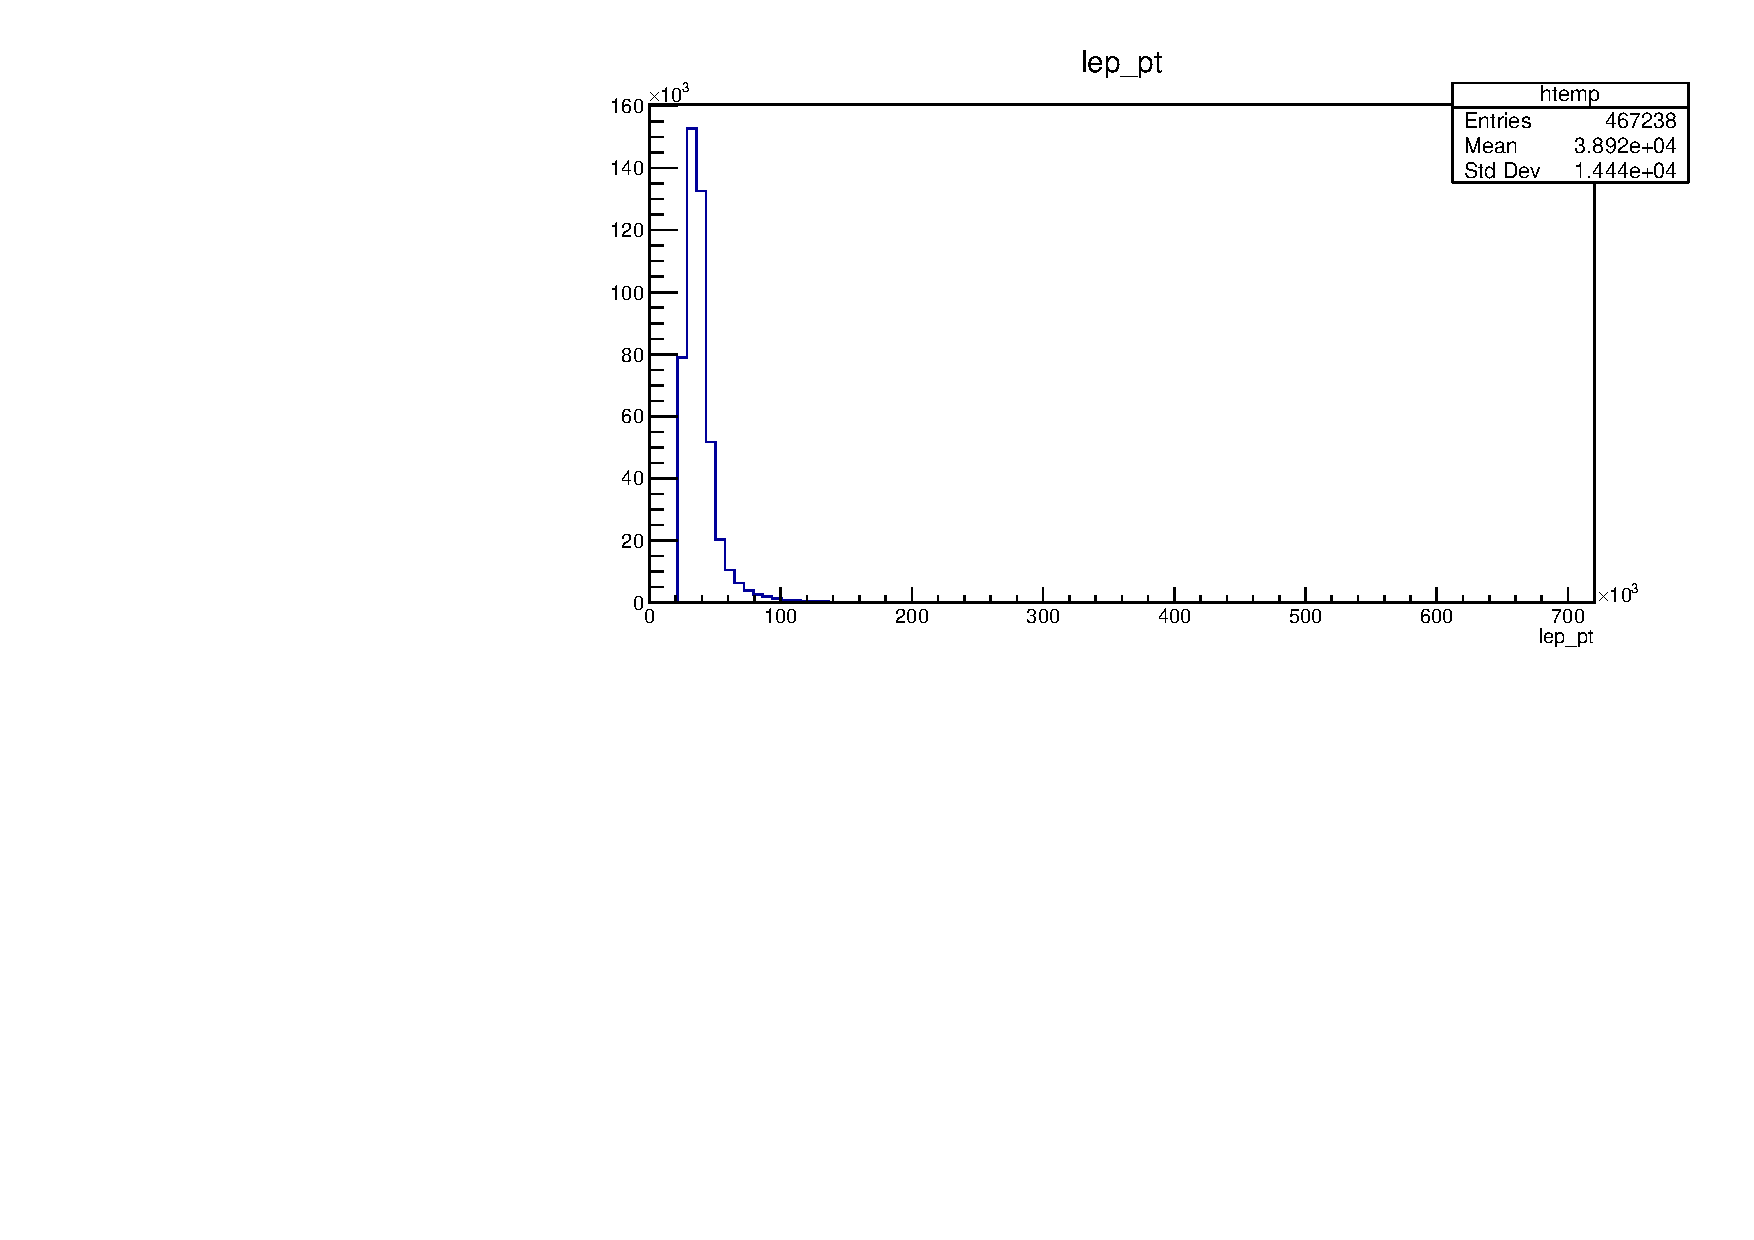
\includegraphics[width=.9\textwidth]{plots/TBrowser_hist.pdf}
    \caption{Histogram of the transverse momentum of the leptons in from one of the data samples created with the \texttt{TBrowser} environment from \texttt{Root}.}
    \label{fig:unselected_pt}
  \end{figure}

\subsection{The event selection}
To increase the signal to background ratio of the data samples a selection is applied which specifically targets the final state of the \texttt{lepton+jets} 
channel. The final state consists of one charged lepton, a neutrino, two bottom quarks and two other quarks from the 
decay of a W boson. The selection consists of 7 cuts which are applied to tha data samples after each other. 
The efficiency of the selection $(A \cdot \epsilon) = \# \text{events(after cut)} / \# \text{events(before cut)}$ of every cut together with all 
cuts that have been applied beforehand is listed in table \ref{tab:eff_a} and \ref{tab:eff_b} for all monte carlo samples.\\
For the jets the number of good jets in one event has to be $\geq 4$ (Cut 1) while exactly one lepton is required (Cut 2) 
in the events. Since the final state contains a neutrino which is not seen in the detector a missing 
transverse energy $met\_et > 40 \, \si{\giga\eV}$ (Cut 3) is required. To supress combinatorial background 
the lepton is required to have a transverse momentum $lep\_pt > 50 \, \si{\giga\eV}$ (Cut 4) and one of 
the jets has to pass $jet\_pt > 80 \, \si{\giga\eV}$ (Cut 5). The number of b-tagged jets in one event has to be 
$\geq 2$ (Cut 6) and one of the b-jets has to fulfill $\texttt{jet\_pt} > 50 \, \si{\giga\eV}$ (Cut 7).
% original table table with the efficiencies
%\begin{table}[]
%    \begin{tabular}{l|lllllll}
%    sample             & Cut 1 & Cut 2 & Cut 3 & Cut 4     & Cut 5  &  Cut 6 & Cut 7 \\
%    \hline
%      %data.el.0     & 0.00531987 & 0.0051666  & 0.00281875 & 0.00138605  & 0.00101955  & 0.000251    & 0.000228788 \\
%      %data.el.1     & 0.00529988 & 0.0051555  & 0.00279876 & 0.00147935  & 0.00111284  & 0.000288761 & 0.00026877  \\
%      %data.el.2     & 0.00512884 & 0.00501112 & 0.00268104 & 0.00126166  & 0.000937363 & 0.000242115 & 0.000224345 \\
%      %data.el.3     & 0.00531321 & 0.0051866  & 0.00292093 & 0.00148379  & 0.00111506  & 0.000299867 & 0.000279876 \\
%      %data.el.4     & 0.00510885 & 0.00498891 & 0.00269214 & 0.00134829  & 0.00100622  & 0.000255443 & 0.000237673 \\
%      %data.el.5     & 0.00526656 & 0.0050933  & 0.00277655 & 0.00138605  & 0.00108174  & 0.000270991 & 0.000248779 \\
%      %data.el.6     & 0.00499113 & 0.00484452 & 0.00258997 & 0.00130831  & 0.00100622  & 0.000246558 & 0.000224345 \\
%      %data.el.7     & 0.00509997 & 0.00498668 & 0.00267882 & 0.00124834  & 0.000926257 & 0.000253221 & 0.000226566 \\
%      %data.el.8     & 0.00519549 & 0.00505333 & 0.00266105 & 0.00128388  & 0.000966242 & 0.000251001 & 0.000244337 \\
%      %data.el.9     & 0.00529545 & 0.00517328 & 0.00290539 & 0.00147491  & 0.0011506   & 0.000308753 & 0.000286541 \\
%      %data.el       & 0.00520192 & 0.00506598 & 0.00275234 & 0.00136606  & 0.00103221  & 0.000266771 & 0.000247002 \\
%      %data.mu.0     & 0.00456057 & 0.00440073 & 0.00265678 & 0.0012538   & 0.000969653 & 0.000241525 & 0.000223766 \\
%      %data.mu.1     & 0.00438298 & 0.00422848 & 0.00254312 & 0.00119875  & 0.000903946 & 0.000202455 & 0.000190024 \\
%      %data.mu.2     & 0.00458544 & 0.00440074 & 0.00272427 & 0.00129465  & 0.000990966 & 0.000232646 & 0.000213111 \\
%      %data.mu.3     & 0.00442738 & 0.00428708 & 0.00266033 & 0.00125558  & 0.000966103 & 0.000268165 & 0.000248629 \\
%      %data.mu.4     & 0.00448243 & 0.00432082 & 0.00260173 & 0.00124137  & 0.000948344 & 0.000225542 & 0.000204231 \\
%      %data.mu.5     & 0.00454104 & 0.00434746 & 0.00261061 & 0.00121828  & 0.000946568 & 0.000243302 & 0.000225542 \\
%      %data.mu.6     & 0.00447355 & 0.00431727 & 0.00272604 & 0.00129465  & 0.0010176   & 0.000257509 & 0.000243302 \\
%      %data.mu.7     & 0.00431194 & 0.00414501 & 0.00252359 & 0.00126268  & 0.000935912 & 0.000243302 & 0.000232646 \\
%      %data.mu.8     & 0.00454814 & 0.00436522 & 0.00269408 & 0.00124847  & 0.000960775 & 0.00027882  & 0.000255733 \\
%      %data.mu.9     & 0.00439896 & 0.00422848 & 0.00258752 & 0.00119342  & 0.000921705 & 0.000252181 & 0.000232646 \\
%      %data.mu       & 0.00447124 & 0.00430413 & 0.00263281 & 0.00124617  & 0.000956158 & 0.000244545 & 0.000226963 \\
%      diboson.el    & 0.0202309  & 0.0194924  & 0.010668   & 0.00565275  & 0.00371891  & 0.000127506 & 0.00011688  \\
%      diboson.mu    & 0.016195   & 0.0149084  & 0.0093971  & 0.00480721  & 0.00313382  & 9.99691e-05 & 9.56227e-05 \\
%      singletop.el  & 0.0906053  & 0.0899371  & 0.0628734  & 0.0336544   & 0.0262382   & 0.00835954  & 0.00795335  \\
%      singletop.mu  & 0.0890013  & 0.0881404  & 0.0624559  & 0.0311724   & 0.0238848   & 0.00794863  & 0.00747094  \\
%      ttbar.el      & 0.436571   & 0.427593   & 0.307784   & 0.163033    & 0.128469    & 0.053868    & 0.0505078   \\
%      ttbar.mu      & 0.434872   & 0.424322   & 0.306789   & 0.154734    & 0.121542    & 0.0513304   & 0.0482129   \\
%      wjets.el      & 0.00489397 & 0.00489397 & 0.00311956 & 0.00159742  & 0.00125348  & 1.66945e-05 & 1.42213e-05 \\
%      wjets.mu      & 0.00482915 & 0.00482903 & 0.00312312 & 0.00150353  & 0.00115609  & 1.74563e-05 & 1.52894e-05 \\
%      zjets.el      & 0.0118665  & 0.0106797  & 0.00297376 & 0.00170699  & 0.00117077  & 5.65506e-05 & 5.25442e-05 \\
%      zjets.mu      & 0.00627221 & 0.0040402  & 0.0015754  & 0.000833442 & 0.00062556  & 3.62866e-05 & 3.3859e-05  \\
%      zprime400.el  & 0.336048   & 0.330579   & 0.222776   & 0.0988089   & 0.0562713   & 0.0238211   & 0.0226057   \\
%      zprime400.mu  & 0.339518   & 0.335549   & 0.230281   & 0.0935609   & 0.0595297   & 0.0242088   & 0.0222244   \\
%      zprime500.el  & 0.418102   & 0.411958   & 0.298848   & 0.16983     & 0.137905    & 0.0554032   & 0.0502468   \\
%      zprime500.mu  & 0.401054   & 0.394935   & 0.28328    & 0.152137    & 0.122952    & 0.0505555   & 0.0480136   \\
%      zprime750.el  & 0.537326   & 0.524537   & 0.427844   & 0.30235     & 0.293616    & 0.125702    & 0.121439    \\
%      zprime750.mu  & 0.532581   & 0.517974   & 0.424298   & 0.292574    & 0.283128    & 0.127263    & 0.124814    \\
%      zprime1000.el & 0.594403   & 0.581055   & 0.503445   & 0.38859     & 0.383423    & 0.180301    & 0.177395    \\
%      zprime1000.mu & 0.609297   & 0.587992   & 0.50066    & 0.377674    & 0.3716      & 0.168941    & 0.166124    \\
%      zprime1250.el & 0.614838   & 0.597018   & 0.530515   & 0.417424    & 0.413231    & 0.191009    & 0.18798     \\
%      zprime1250.mu & 0.630988   & 0.608626   & 0.537332   & 0.420378    & 0.415793    & 0.19302     & 0.190494    \\
%      zprime1500.el & 0.630429   & 0.610937   & 0.557169   & 0.447279    & 0.443878    & 0.190084    & 0.185767    \\
%      zprime1500.mu & 0.639837   & 0.615859   & 0.555766   & 0.445229    & 0.441747    & 0.188737    & 0.18635     \\
%      zprime1750.el & 0.637424   & 0.619702   & 0.566091   & 0.462266    & 0.458721    & 0.191257    & 0.189632    \\
%      zprime1750.mu & 0.642951   & 0.61898    & 0.565701   & 0.452713    & 0.449444    & 0.189475    & 0.187623    \\
%      zprime2000.el & 0.636319   & 0.613722   & 0.563779   & 0.450139    & 0.446209    & 0.174063    & 0.17177     \\
%      zprime2000.mu & 0.659439   & 0.635841   & 0.58541    & 0.468376    & 0.464902    & 0.180283    & 0.179085    \\
%      zprime2250.el & 0.63421    & 0.614402   & 0.567938   & 0.448538    & 0.446316    & 0.168456    & 0.16716     \\
%      zprime2250.mu & 0.652435   & 0.628021   & 0.580443   & 0.471391    & 0.468386    & 0.180669    & 0.178165    \\
%      zprime2500.el & 0.636889   & 0.618791   & 0.56315    & 0.442434    & 0.438776    & 0.1598      & 0.157682    \\
%      zprime2500.mu & 0.658653   & 0.635011   & 0.585602   & 0.471245    & 0.466729    & 0.175721    & 0.172799    \\
%      zprime3000.el & 0.6        & 0.584015   & 0.524453   & 0.394481    & 0.385728    & 0.147288    & 0.145005    \\
%      zprime3000.mu & 0.626332   & 0.604459   & 0.546971   & 0.430875    & 0.424285    & 0.160684    & 0.15816     
%    \end{tabular}
%    \end{table}

%\begin{figure}

  \begin{table}[H]
    \centering
    \begin{tabular}{l|lllllll}
    sample             & Cut 1 & Cut 2 & Cut 3 & Cut 4     & Cut 5   \\
    \hline
      diboson.el    & 0.0202309  & 0.0194924  & 0.010668   & 0.00565275  & 0.00371891  \\
      diboson.mu    & 0.016195   & 0.0149084  & 0.0093971  & 0.00480721  & 0.00313382  \\
      singletop.el  & 0.0906053  & 0.0899371  & 0.0628734  & 0.0336544   & 0.0262382   \\
      singletop.mu  & 0.0890013  & 0.0881404  & 0.0624559  & 0.0311724   & 0.0238848   \\
      ttbar.el      & 0.436571   & 0.427593   & 0.307784   & 0.163033    & 0.128469    \\
      ttbar.mu      & 0.434872   & 0.424322   & 0.306789   & 0.154734    & 0.121542    \\
      wjets.el      & 0.00489397 & 0.00489397 & 0.00311956 & 0.00159742  & 0.00125348  \\
      wjets.mu      & 0.00482915 & 0.00482903 & 0.00312312 & 0.00150353  & 0.00115609  \\
      zjets.el      & 0.0118665  & 0.0106797  & 0.00297376 & 0.00170699  & 0.00117077  \\
      zjets.mu      & 0.00627221 & 0.0040402  & 0.0015754  & 0.000833442 & 0.00062556  \\
      zprime400.el  & 0.336048   & 0.330579   & 0.222776   & 0.0988089   & 0.0562713   \\
      zprime400.mu  & 0.339518   & 0.335549   & 0.230281   & 0.0935609   & 0.0595297   \\
      zprime500.el  & 0.418102   & 0.411958   & 0.298848   & 0.16983     & 0.137905    \\
      zprime500.mu  & 0.401054   & 0.394935   & 0.28328    & 0.152137    & 0.122952    \\
      zprime750.el  & 0.537326   & 0.524537   & 0.427844   & 0.30235     & 0.293616    \\
      zprime750.mu  & 0.532581   & 0.517974   & 0.424298   & 0.292574    & 0.283128    \\
      zprime1000.el & 0.594403   & 0.581055   & 0.503445   & 0.38859     & 0.383423    \\
      zprime1000.mu & 0.609297   & 0.587992   & 0.50066    & 0.377674    & 0.3716      \\
      zprime1250.el & 0.614838   & 0.597018   & 0.530515   & 0.417424    & 0.413231    \\
      zprime1250.mu & 0.630988   & 0.608626   & 0.537332   & 0.420378    & 0.415793    \\
      zprime1500.el & 0.630429   & 0.610937   & 0.557169   & 0.447279    & 0.443878    \\
      zprime1500.mu & 0.639837   & 0.615859   & 0.555766   & 0.445229    & 0.441747    \\
      zprime1750.el & 0.637424   & 0.619702   & 0.566091   & 0.462266    & 0.458721    \\
      zprime1750.mu & 0.642951   & 0.61898    & 0.565701   & 0.452713    & 0.449444    \\
      zprime2000.el & 0.636319   & 0.613722   & 0.563779   & 0.450139    & 0.446209    \\
      zprime2000.mu & 0.659439   & 0.635841   & 0.58541    & 0.468376    & 0.464902    \\
      zprime2250.el & 0.63421    & 0.614402   & 0.567938   & 0.448538    & 0.446316    \\
      zprime2250.mu & 0.652435   & 0.628021   & 0.580443   & 0.471391    & 0.468386    \\
      zprime2500.el & 0.636889   & 0.618791   & 0.56315    & 0.442434    & 0.438776    \\
      zprime2500.mu & 0.658653   & 0.635011   & 0.585602   & 0.471245    & 0.466729    \\
      zprime3000.el & 0.6        & 0.584015   & 0.524453   & 0.394481    & 0.385728    \\
      zprime3000.mu & 0.626332   & 0.604459   & 0.546971   & 0.430875    & 0.424285    
    \end{tabular}
    %\end{table}
    \caption{The efficiency of the selection after the application of subsequent cuts (1-5).}
    \label{tab:eff_a}

  \end{table}


\begin{table}[H]
  \centering
  \begin{tabular}{l|ll}
      sample           & Cut 6  & Cut 7 \\
      \hline
      diboson.el    & 0.000127506 & 0.00011688  \\
      diboson.mu    & 9.99691e-05 & 9.56227e-05 \\
      singletop.el  & 0.00835954  & 0.00795335  \\
      singletop.mu  & 0.00794863  & 0.00747094  \\
      ttbar.el      & 0.053868    & 0.0505078   \\
      ttbar.mu      & 0.0513304   & 0.0482129   \\
      wjets.el      & 1.66945e-05 & 1.42213e-05 \\
      wjets.mu      & 1.74563e-05 & 1.52894e-05 \\
      zjets.el      & 5.65506e-05 & 5.25442e-05 \\
      zjets.mu      & 3.62866e-05 & 3.3859e-05  \\
      zprime400.el  & 0.0238211   & 0.0226057   \\
      zprime400.mu  & 0.0242088   & 0.0222244   \\
      zprime500.el  & 0.0554032   & 0.0502468   \\
      zprime500.mu  & 0.0505555   & 0.0480136   \\
      zprime750.el  & 0.125702    & 0.121439    \\
      zprime750.mu  & 0.127263    & 0.124814    \\
      zprime1000.el & 0.180301    & 0.177395    \\
      zprime1000.mu & 0.168941    & 0.166124    \\
      zprime1250.el & 0.191009    & 0.18798     \\
      zprime1250.mu & 0.19302     & 0.190494    \\
      zprime1500.el & 0.190084    & 0.185767    \\
      zprime1500.mu & 0.188737    & 0.18635     \\
      zprime1750.el & 0.191257    & 0.189632    \\
      zprime1750.mu & 0.189475    & 0.187623    \\
      zprime2000.el & 0.174063    & 0.17177     \\
      zprime2000.mu & 0.180283    & 0.179085    \\
      zprime2250.el & 0.168456    & 0.16716     \\
      zprime2250.mu & 0.180669    & 0.178165    \\
      zprime2500.el & 0.1598      & 0.157682    \\
      zprime2500.mu & 0.175721    & 0.172799    \\
      zprime3000.el & 0.147288    & 0.145005    \\
      zprime3000.mu & 0.160684    & 0.15816     
      \end{tabular}
\caption{The efficiency of the selection after the application of subsequent cuts (6-7).}
\label{tab:eff_b}

  \end{table}


\subsection{Fundamental distributions} \label{sec:sekunde}
The main background after the selection is $t \overline{t}$-production due to its similar finlal state which leads to a large selection efficiency 
in table \ref{tab:eff_b} compared to the other simulated Standard Model processes. 
Therefore the $t \overline{t}$-sample is investigated by creating 
histograms of several of the variables for the electron- and muon-samples 
and investigating those for deviations from the expectation of a $t \overline{t}$-sample. 
The chosen distributions are 
\begin{itemize}
  \item the lepton $p_T$, $\eta$, $\phi$ and E,
  \item $p_T$, $\eta$, $\phi$ and E  of all good jets,
  \item the number of good jets in each event, 
  \item $p_T$, $\eta$, $\phi$ and E of the jets with the largest $p_T$ for each event,
  \item the number of b-tagged jets, 
  \item the magnitude of the missing transverse momentum, 
\end{itemize}
where $p_T$ refers to the transverse momentum, $\eta$ to the pseudorapidity, $\phi$ to the azimuthal angle and E to the energy. 
Some of the distributions are shown in figure \ref{fig:2}, figure \ref{fig:3} and figure \ref{fig:4} for the simulated $t\overline{t}$-sample. \\
Both the missing transverse momentum and the transverse momentum shown in figure \ref{fig:2} fall exponentially and appear very similar. 
This agrees with the expectation that the missing transverse momentum should in magnitude be roughly the same since the missing 
transverse momentum should be dominated by the momentum of the neutrino from the W-decay. \\
Both the number of good jets in an event and the number of b-tagged jets have a very similar distribution for the electron- and muon data samples, as 
expected. The same is observed for the kinematic quantities of the jet with the largest transverse momentum of each event. All considered variacles follow 
the expected distribution. 
% only distributions with very specific signatures 
% 4 lep pt and met_et
% 4 number good, b-tagged
% only e one eta, phi ->largest pt jet

\begin{figure}[H]%
  \begin{subfigure}{0.5\textwidth}%
    \centering%
    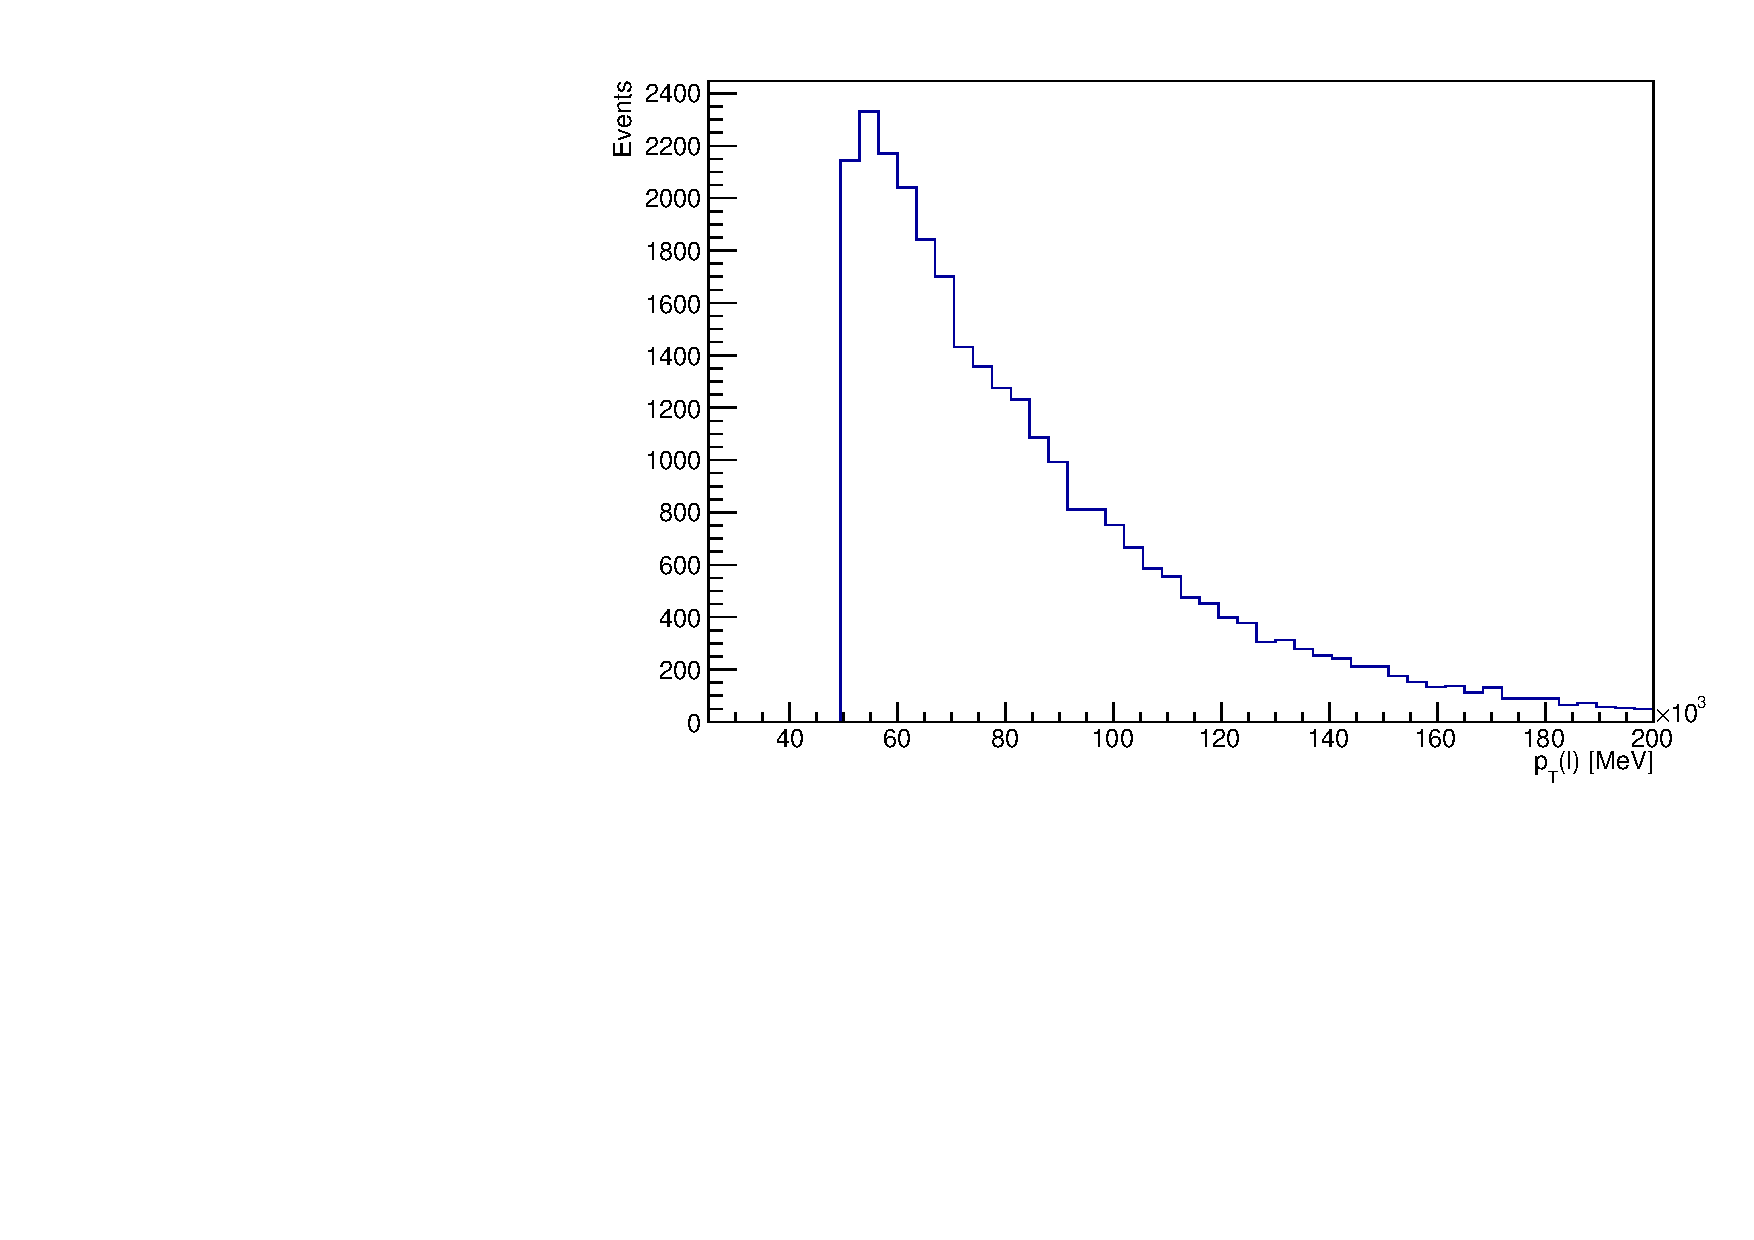
\includegraphics[width=\textwidth]{plots/ttbar_distributions/ttbar.el_lep_pt.pdf}%
    \caption{Transverse momentum of lepton in events where the lepton was tagged as electron.}%
    \label{fig:2a}%
  \end{subfigure}%
  \hfill
  \begin{subfigure}{0.5\textwidth}%
    \centering%
    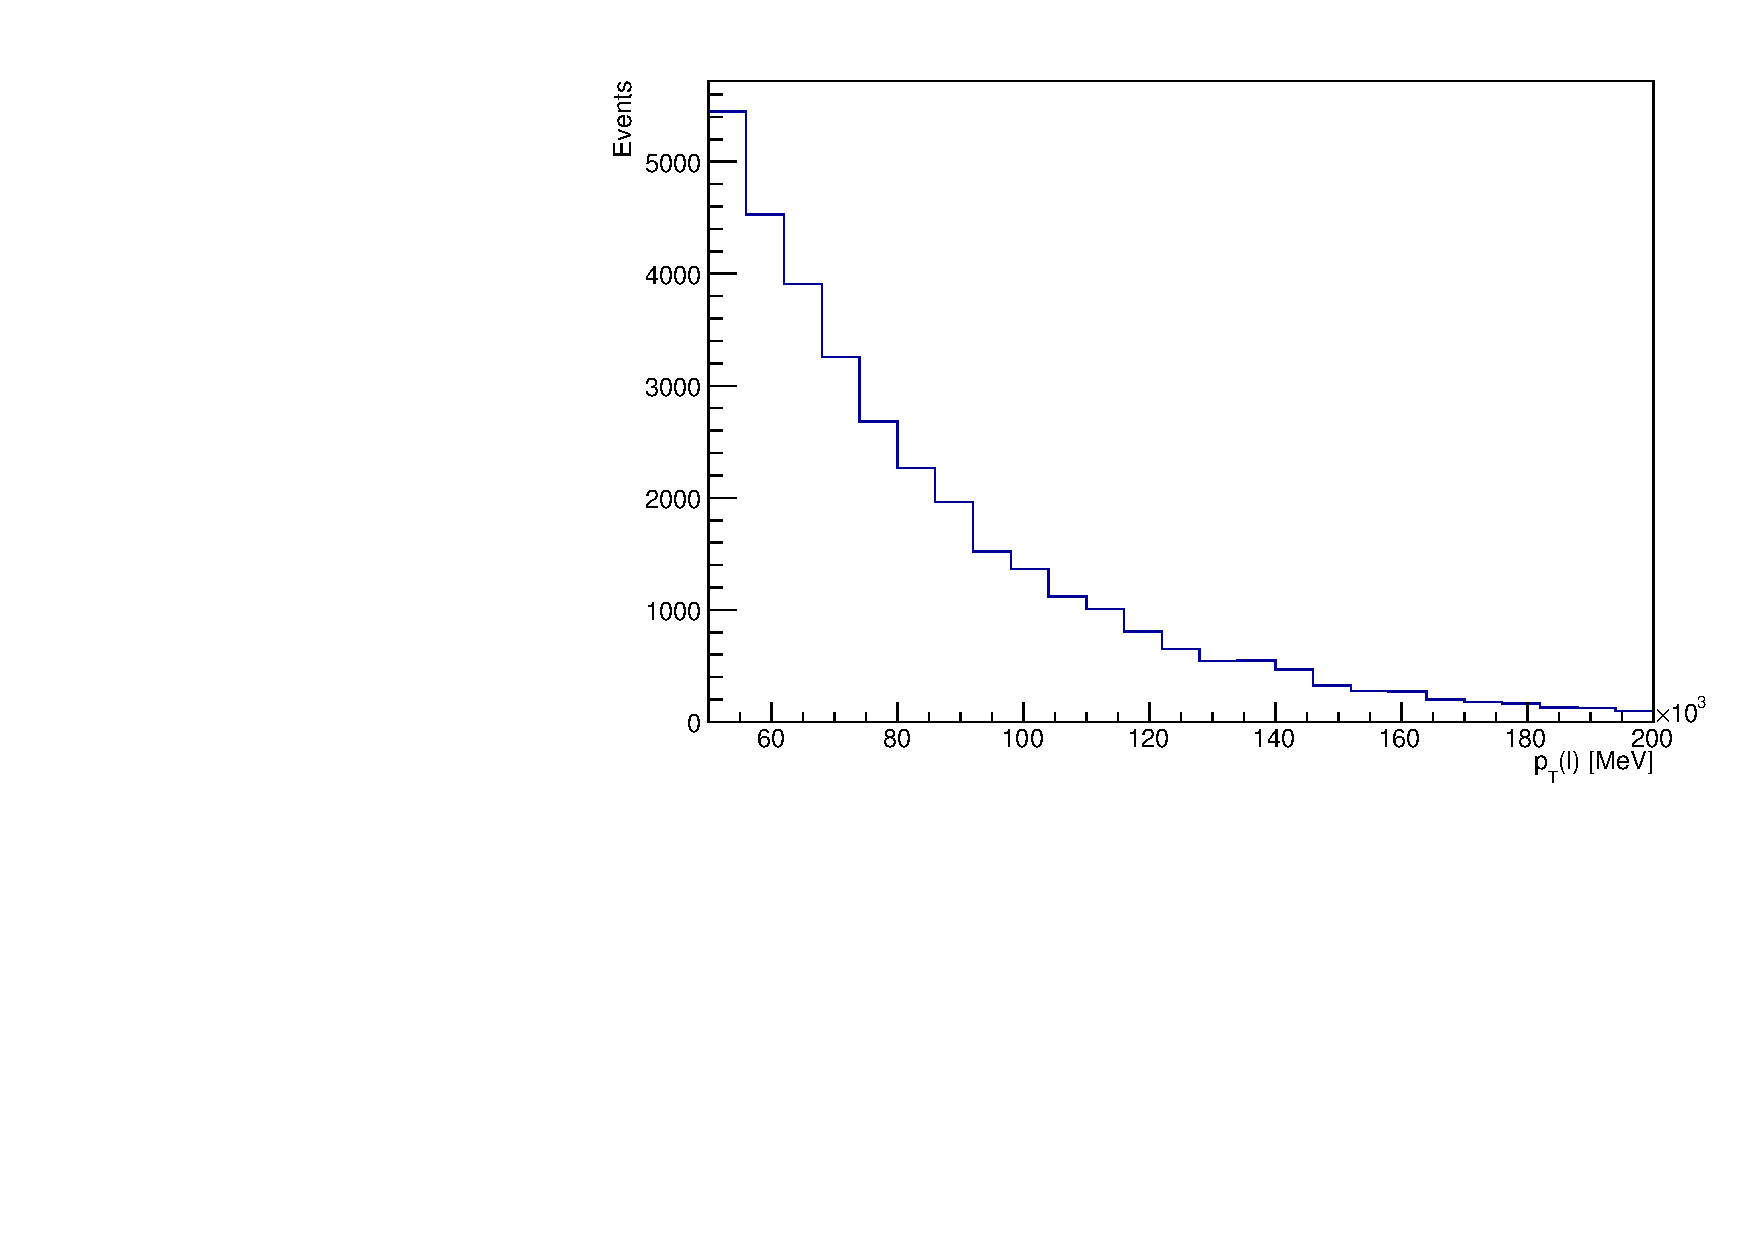
\includegraphics[width=\textwidth]{plots/ttbar_distributions/ttbar.mu_lep_pt.pdf}%
    \caption{Transverse momentum of lepton in events where the lepton was tagged as muon.}%
    \label{fig:2b}%
  \end{subfigure}%

  \begin{subfigure}{0.5\textwidth}%
    \centering%
    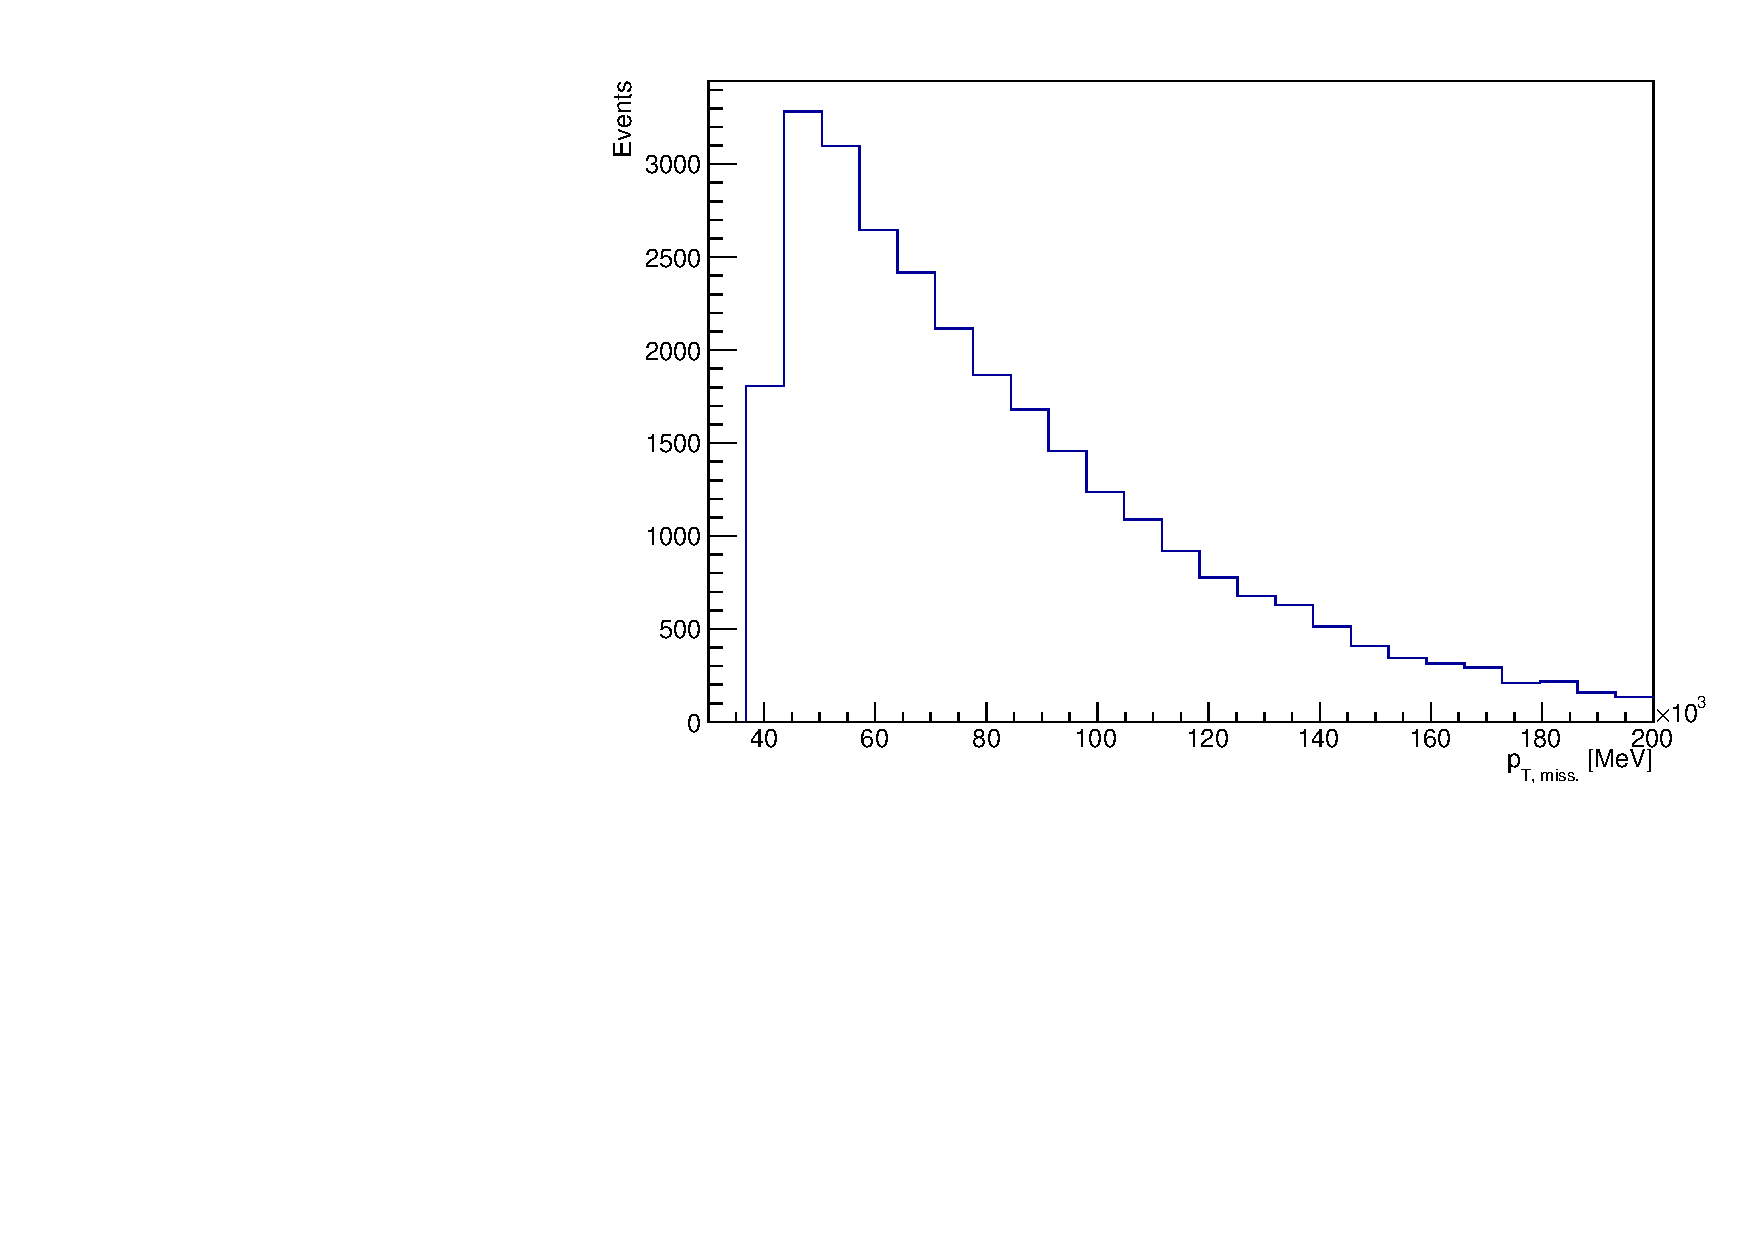
\includegraphics[width=\textwidth]{plots/ttbar_distributions/ttbar.el_met_et.pdf}%
    \caption{Missing transverse energy of events where the lepton was tagged as electron.}%
    \label{fig:2c}%
  \end{subfigure}%
  \hfill
  \begin{subfigure}{0.5\textwidth}%
    \centering%
    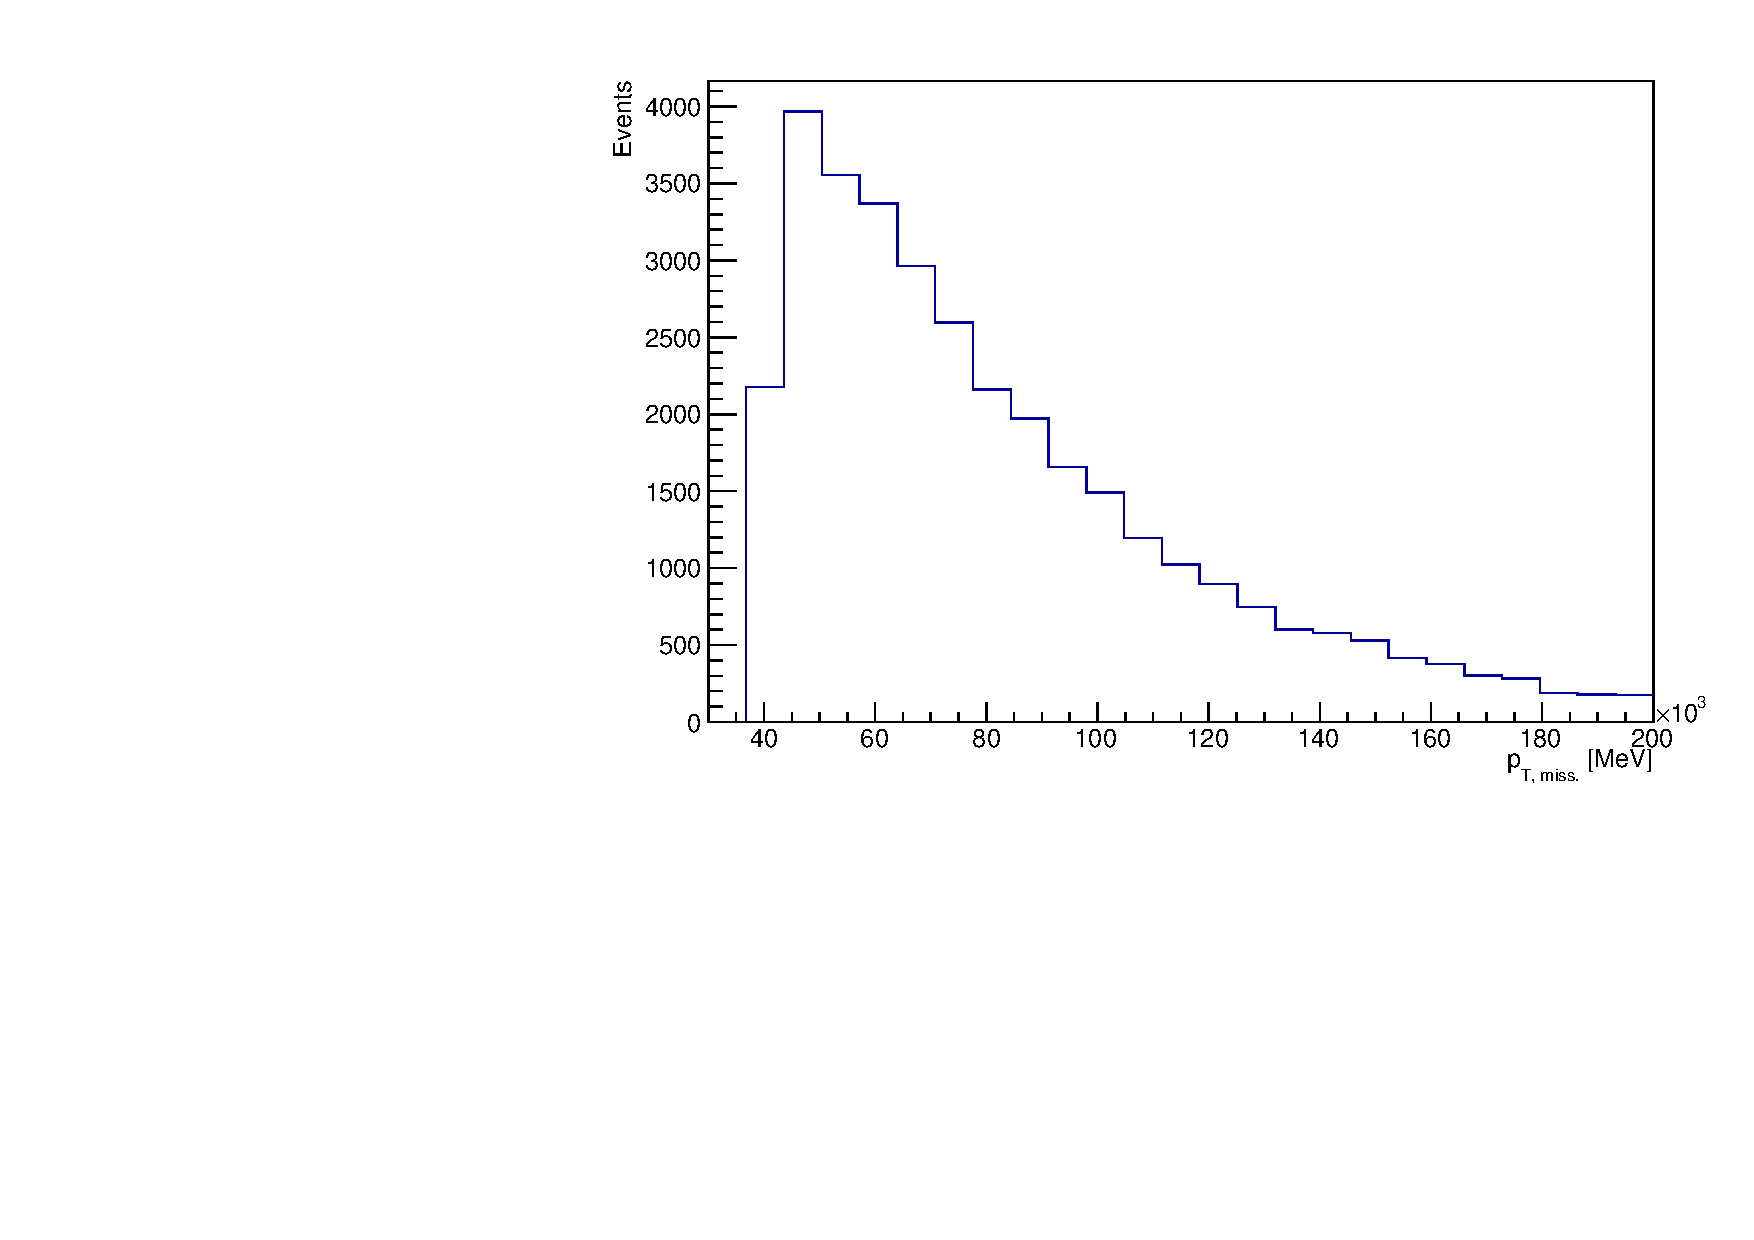
\includegraphics[width=\textwidth]{plots/ttbar_distributions/ttbar.mu_met_et.pdf}%
    \caption{Missing transverse energy of events where the lepton was tagged as muon.}%
    \label{fig:2d}%
  \end{subfigure}%
  \caption{Missing transverse energy of the electron and missing transverse energy of each event.}%
  \label{fig:2}%
\end{figure}


\begin{figure}[H]%
  \begin{subfigure}{0.48\textwidth}%
    \centering%
    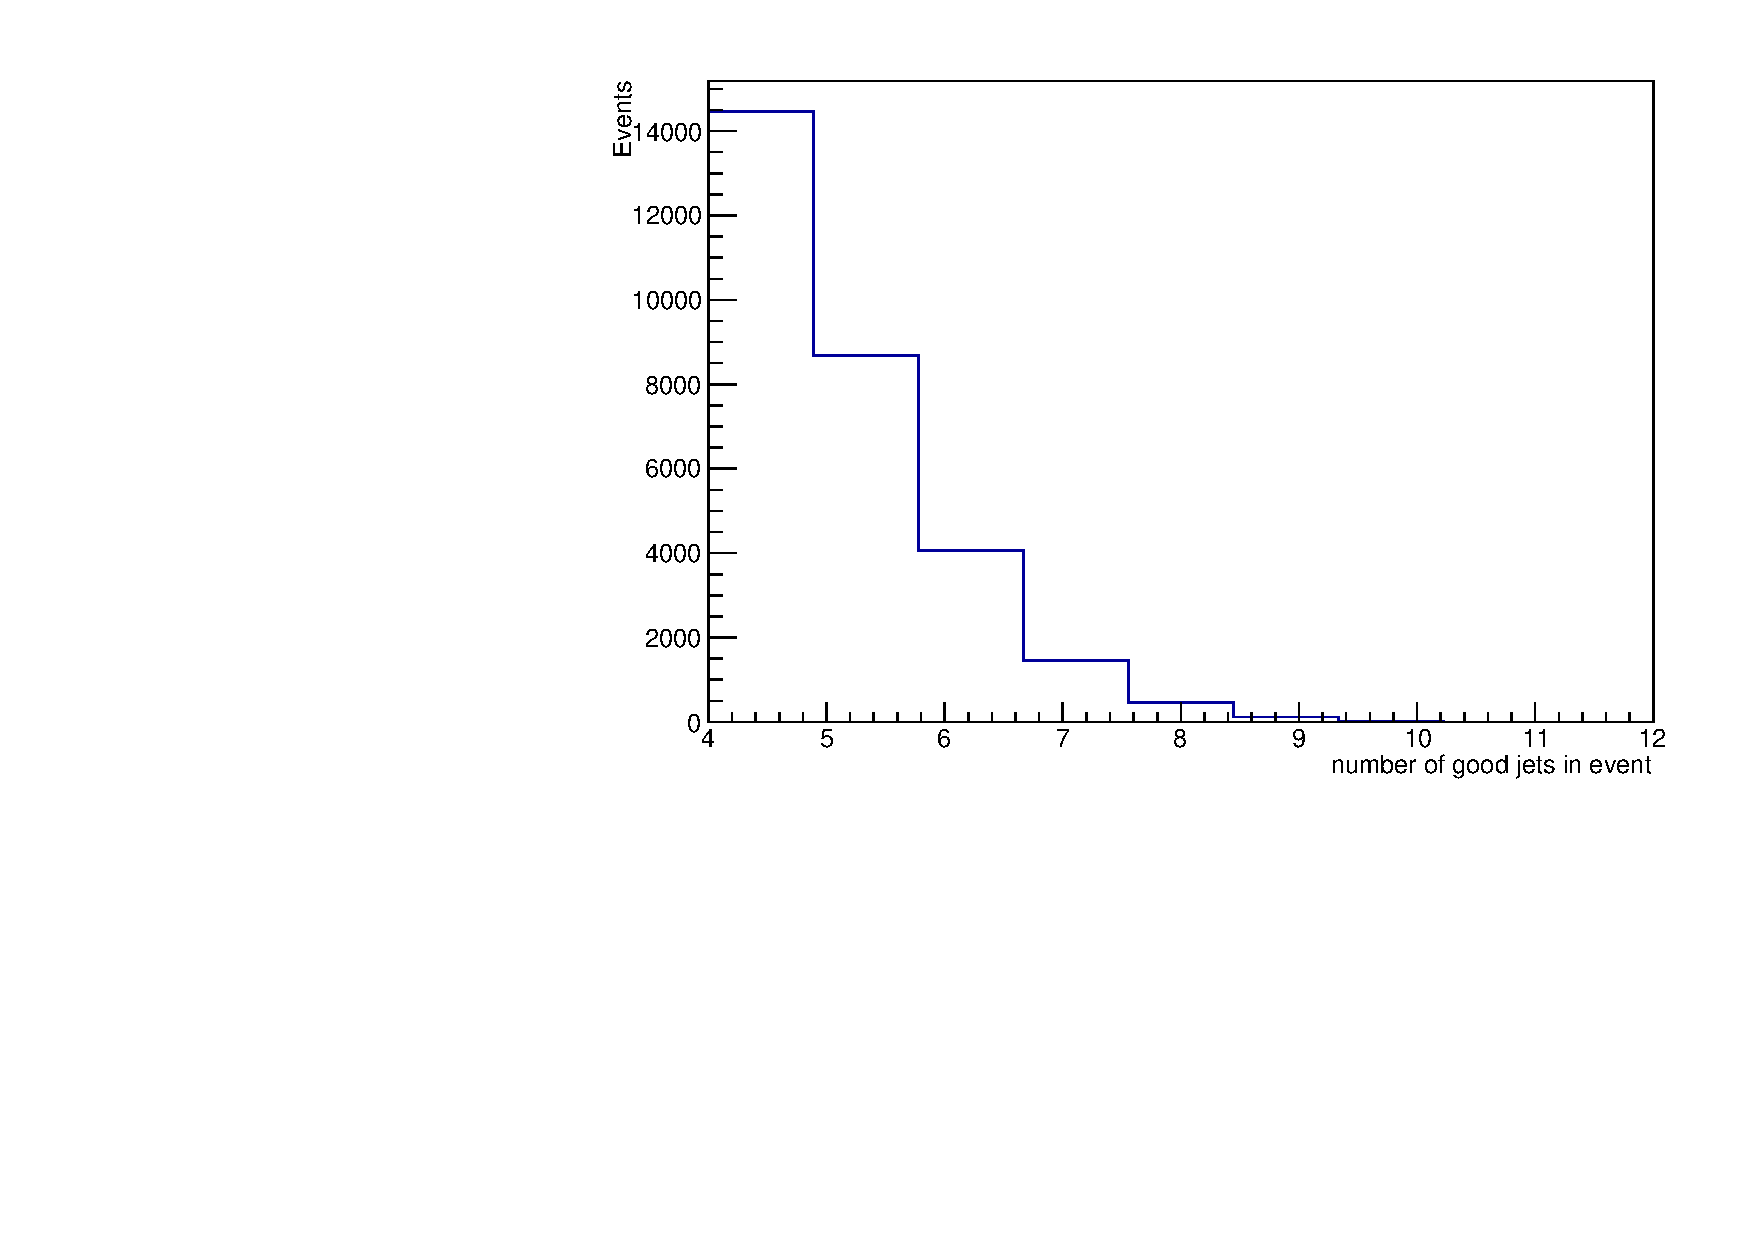
\includegraphics[width=\textwidth]{plots/ttbar_distributions/ttbar.el_jet_good.pdf}%
    \caption{Number of good jets for events where the lepton was tagged as electron.}%
    \label{fig:3a}%
  \end{subfigure}%
  \hfill
  \begin{subfigure}{0.48\textwidth}%
    \centering%
    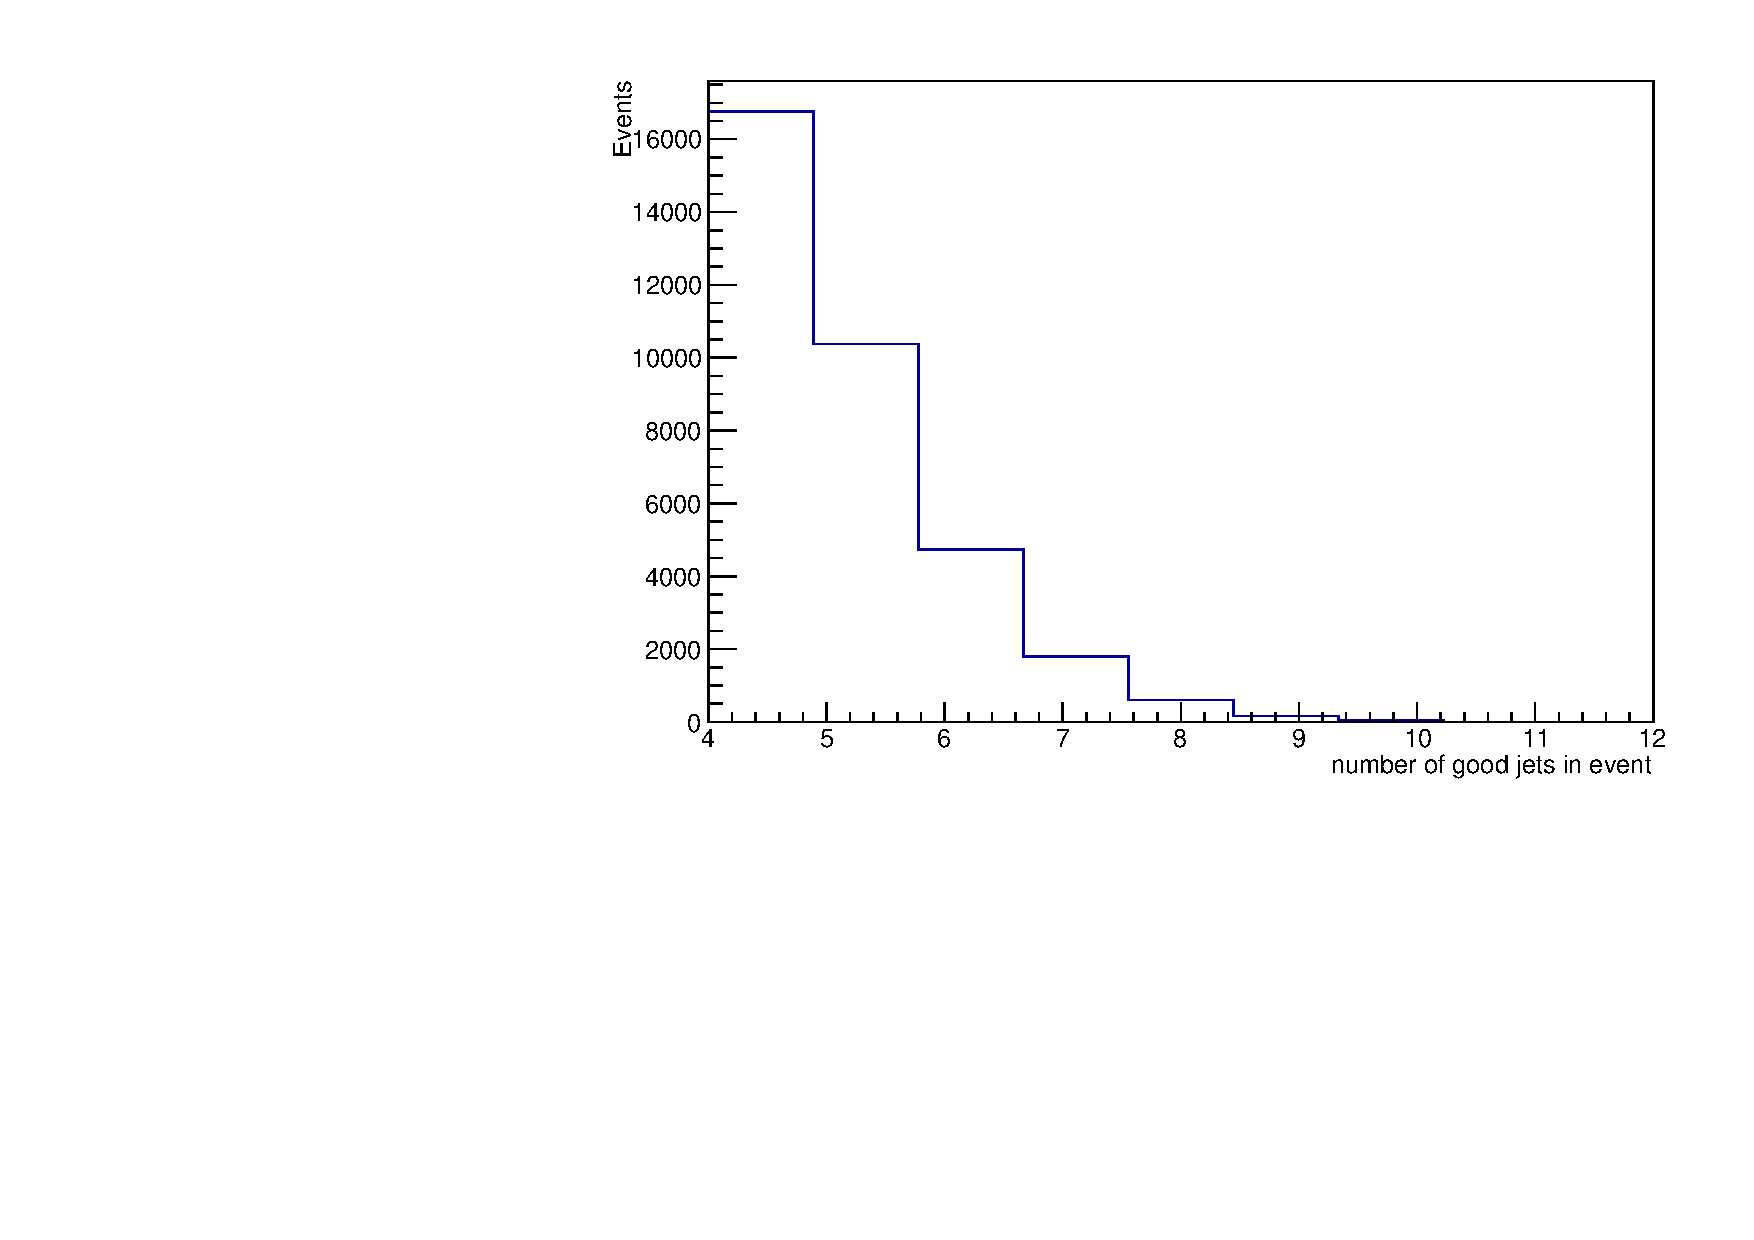
\includegraphics[width=\textwidth]{plots/ttbar_distributions/ttbar.mu_jet_good.pdf}%
    \caption{Number of good jets for events where the lepton was tagged as muon.}%
    \label{fig:3b}%
  \end{subfigure}%

  \begin{subfigure}{0.48\textwidth}%
    \centering%
    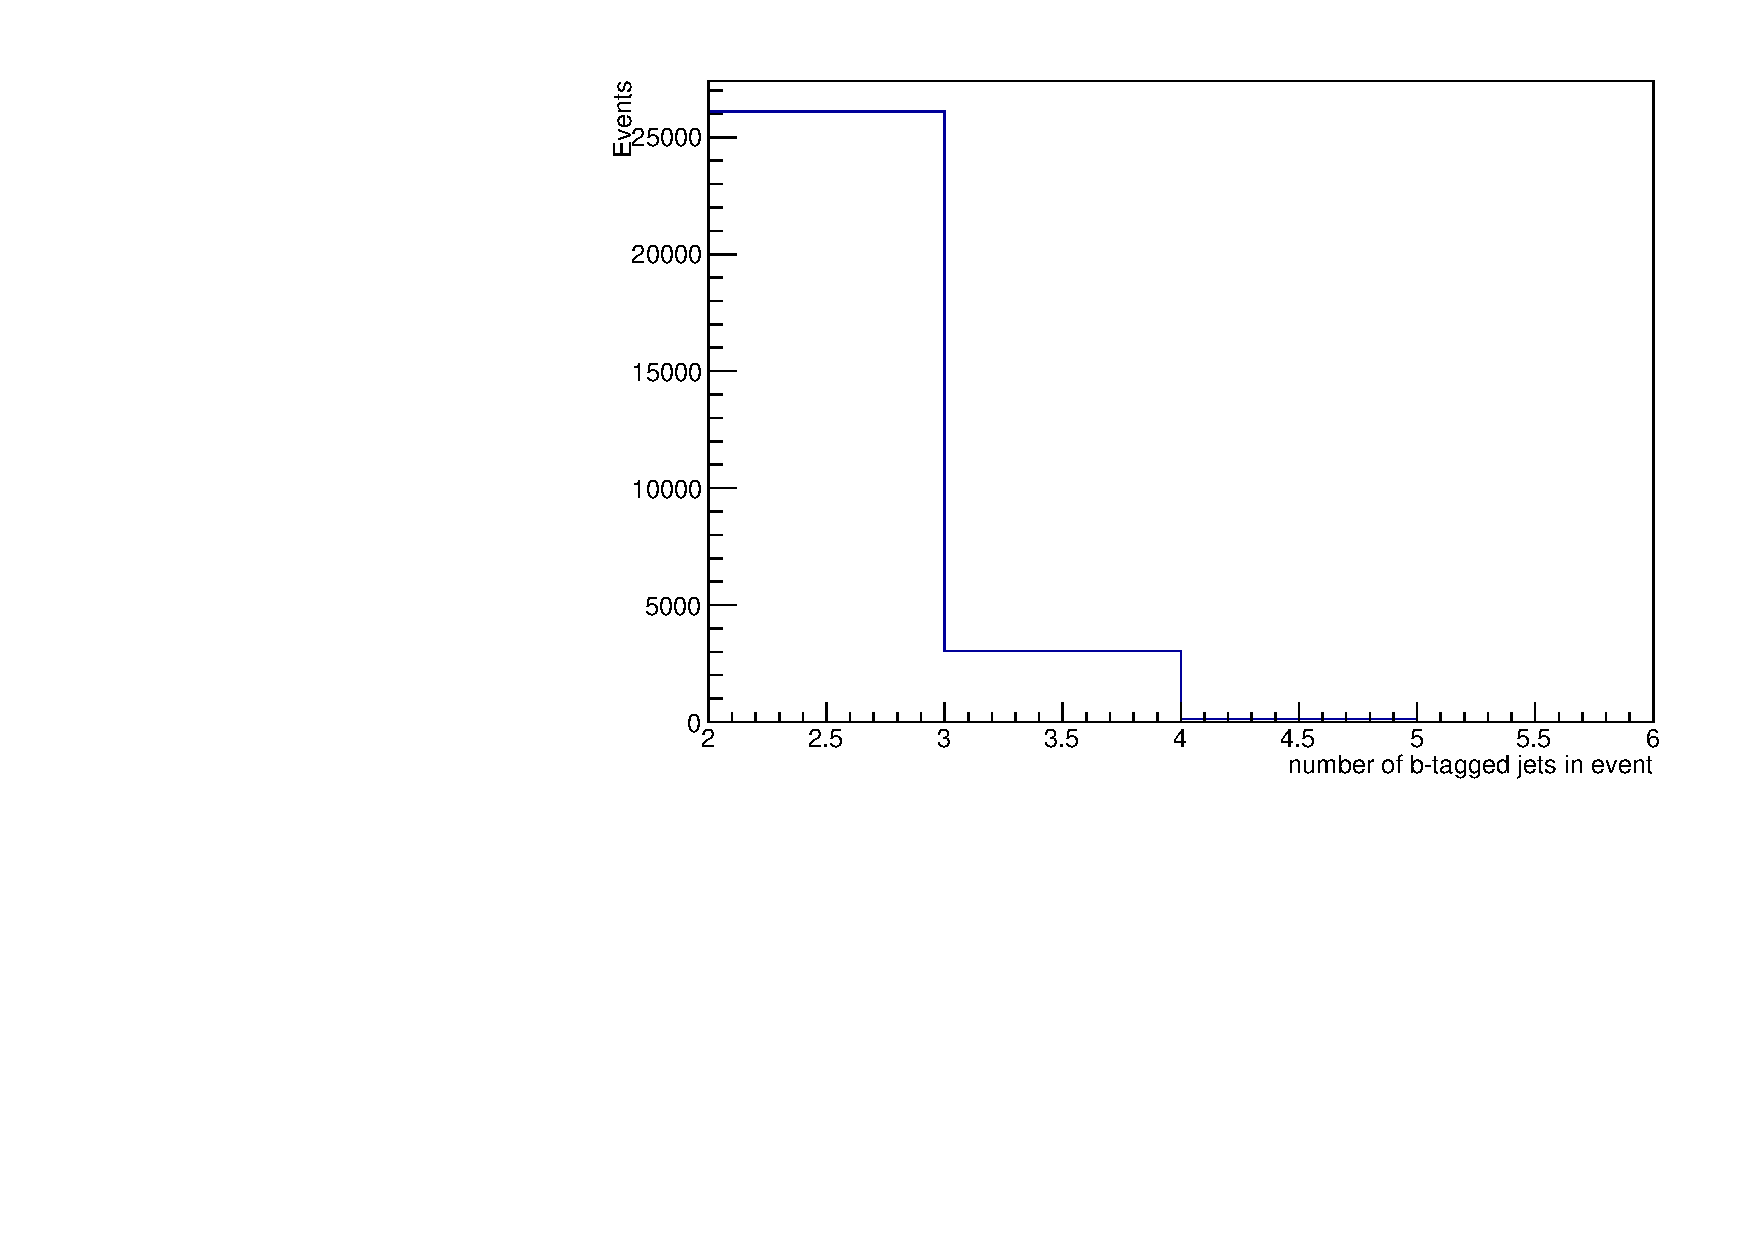
\includegraphics[width=\textwidth]{plots/ttbar_distributions/ttbar.el_jet_btag.pdf}%
    \caption{Number of b-tagged jets for events where the lepton was tagged as electron.}%
    \label{fig:3c}%
  \end{subfigure}%
  \hfill
  \begin{subfigure}{0.48\textwidth}%
    \centering%
    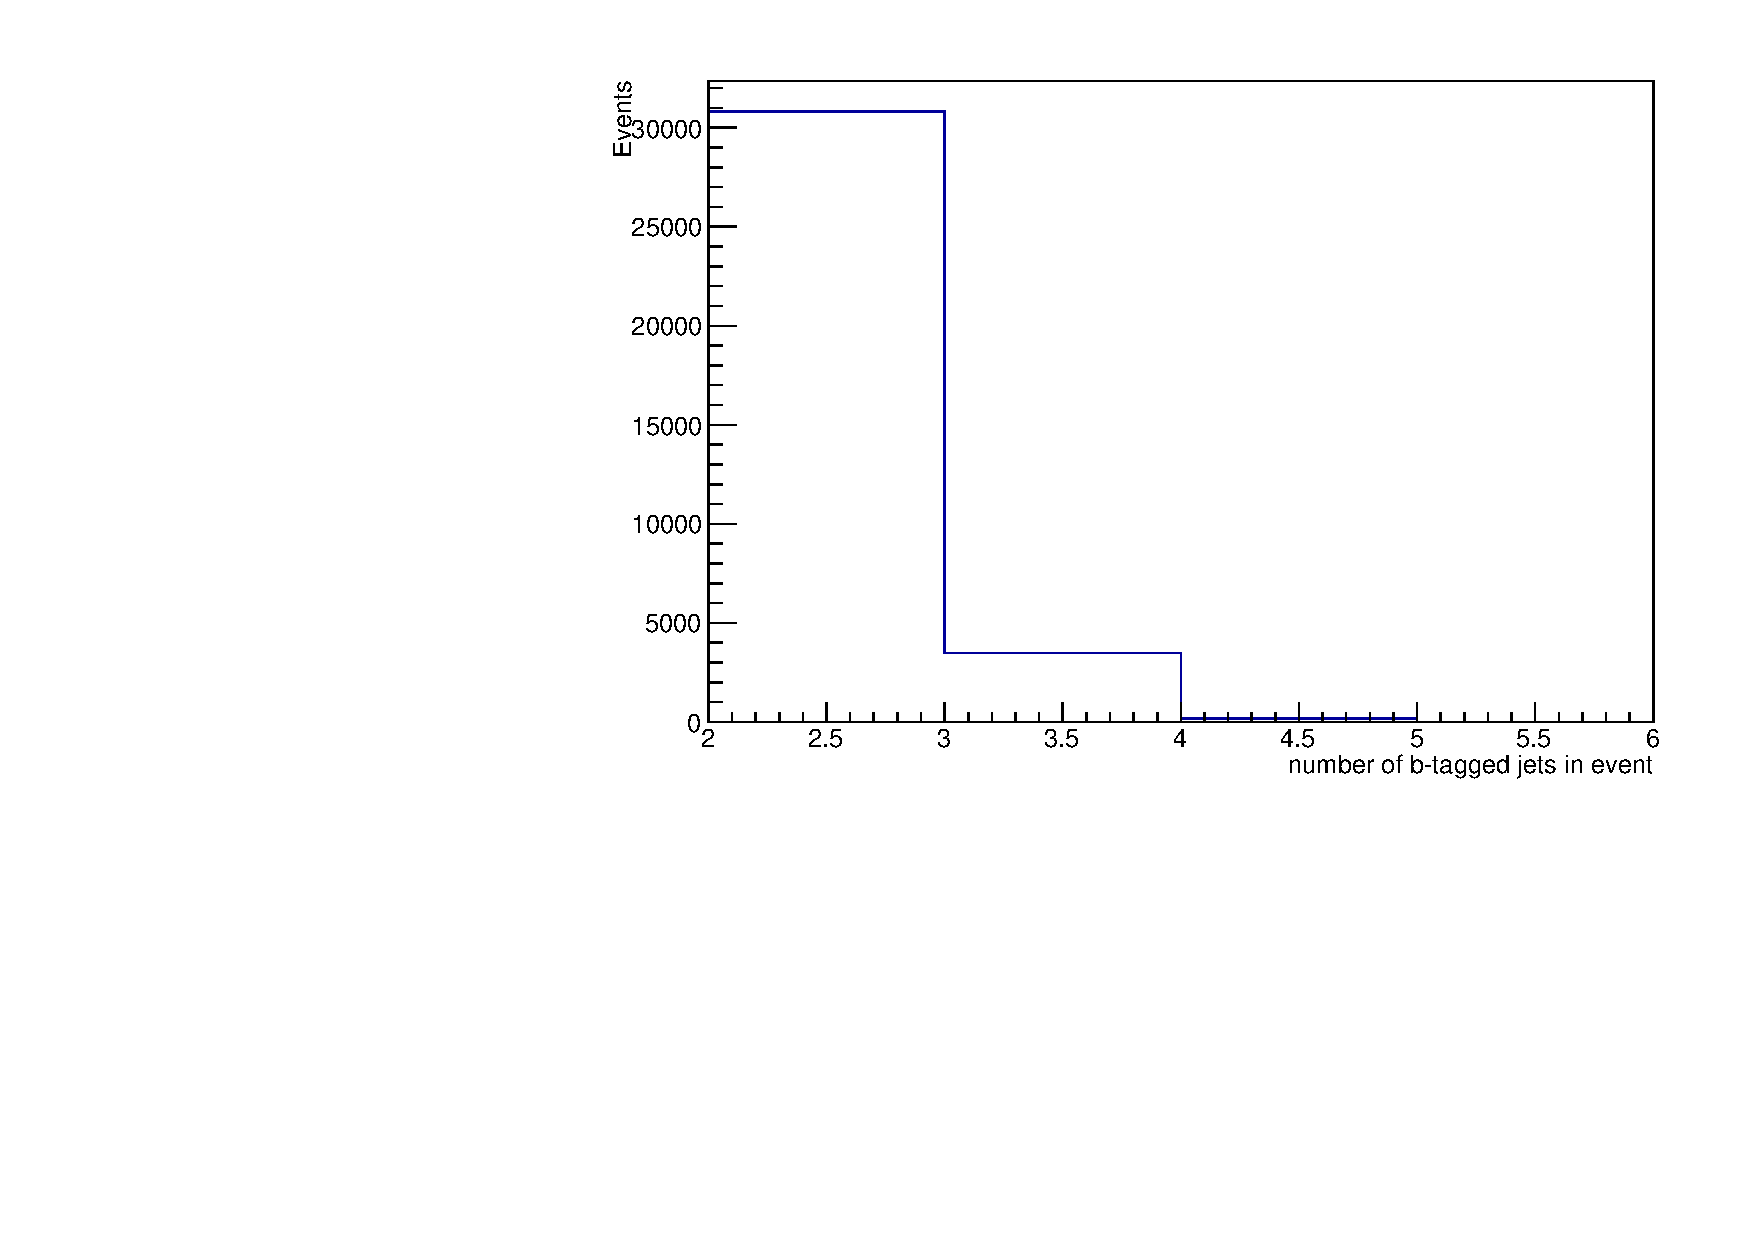
\includegraphics[width=\textwidth]{plots/ttbar_distributions/ttbar.mu_jet_btag.pdf}%
    \caption{Number of b-tagged jets for events where the lepton was tagged as muon.}%
    \label{fig:3d}%
  \end{subfigure}%
  \caption{Number of good jets and b-tagged jets in events.}%
  \label{fig:3}%
\end{figure}

\begin{figure}[H]%
  \begin{subfigure}{0.48\textwidth}%
    \centering%
    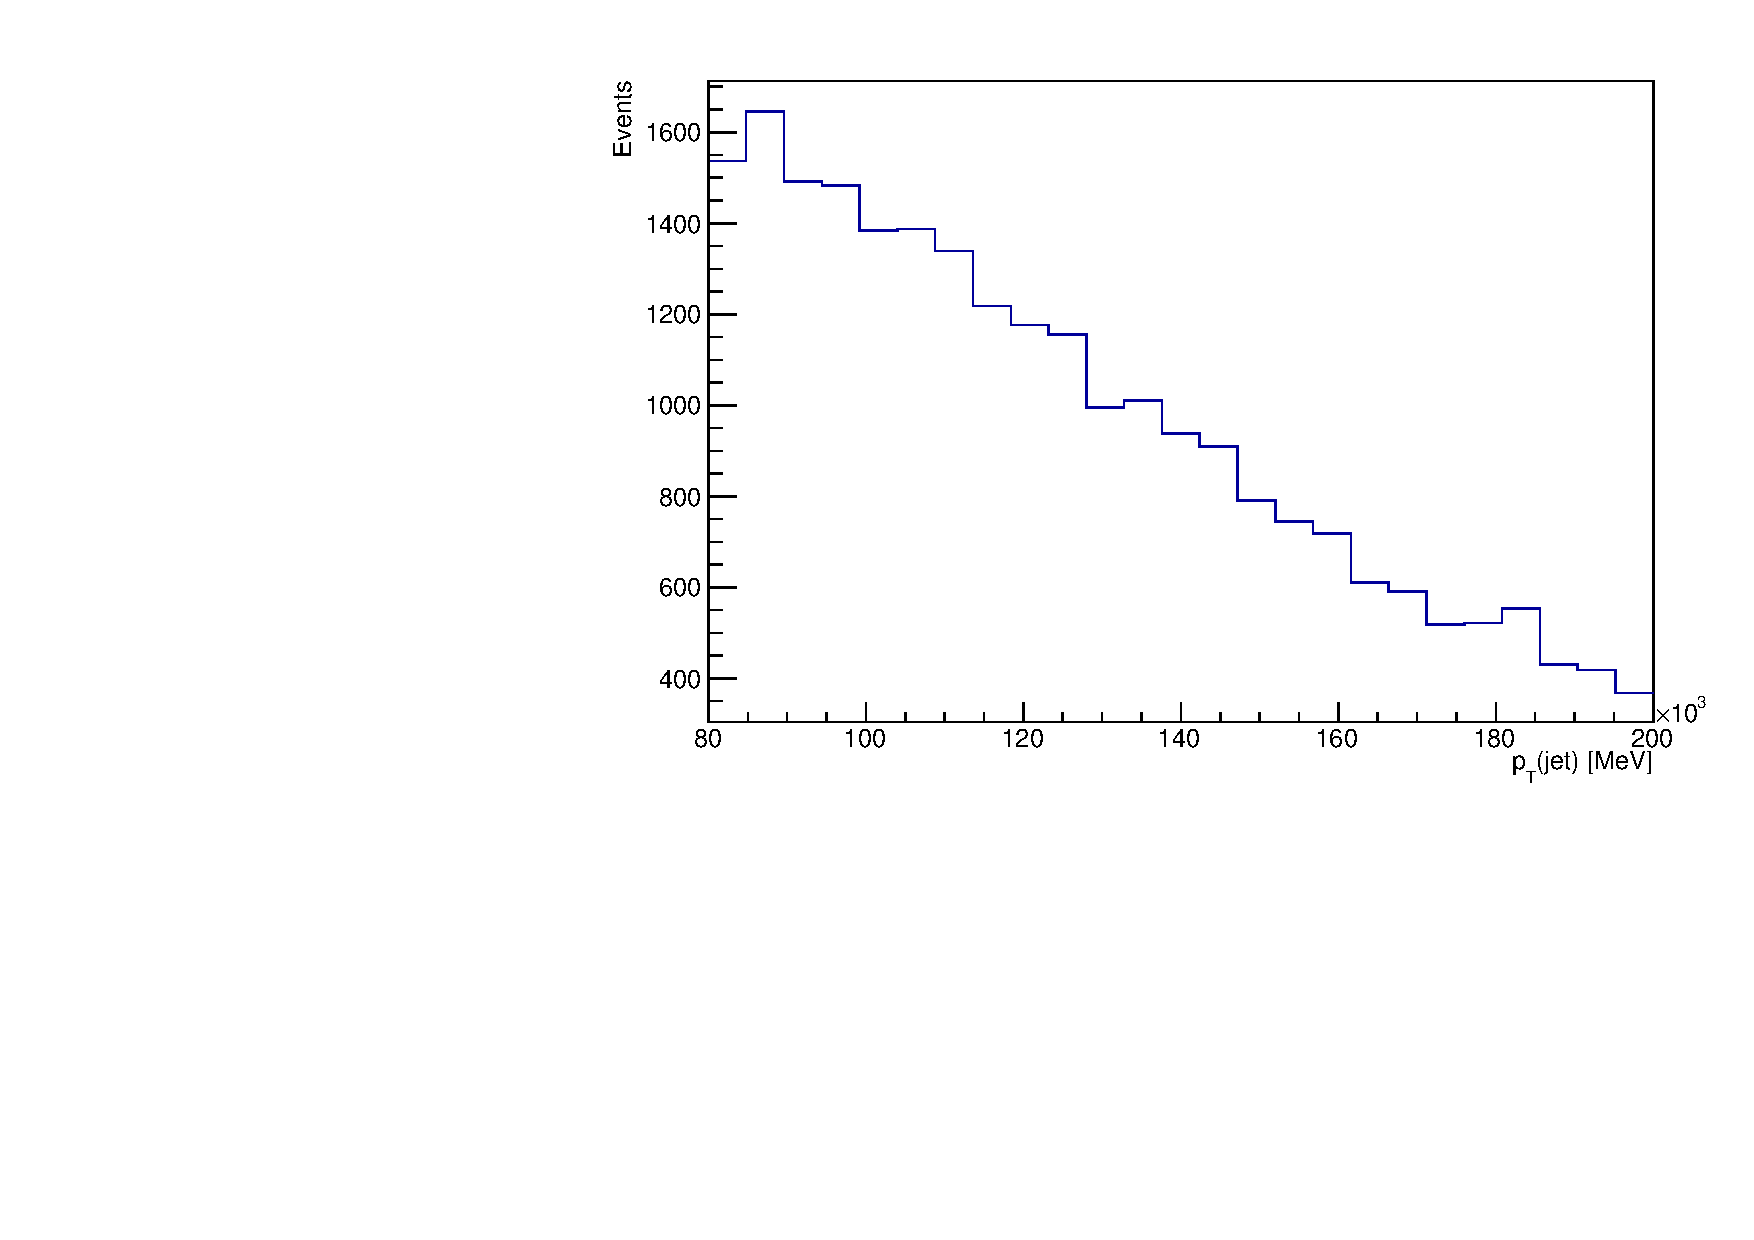
\includegraphics[width=\textwidth]{plots/ttbar_distributions/ttbar.el_jet_pt_max.pdf}%
    \caption{Transverse momentum, lepton is electron.}%
    \label{fig:4a}%
  \end{subfigure}%
  \hfill
  \begin{subfigure}{0.48\textwidth}%
    \centering%
    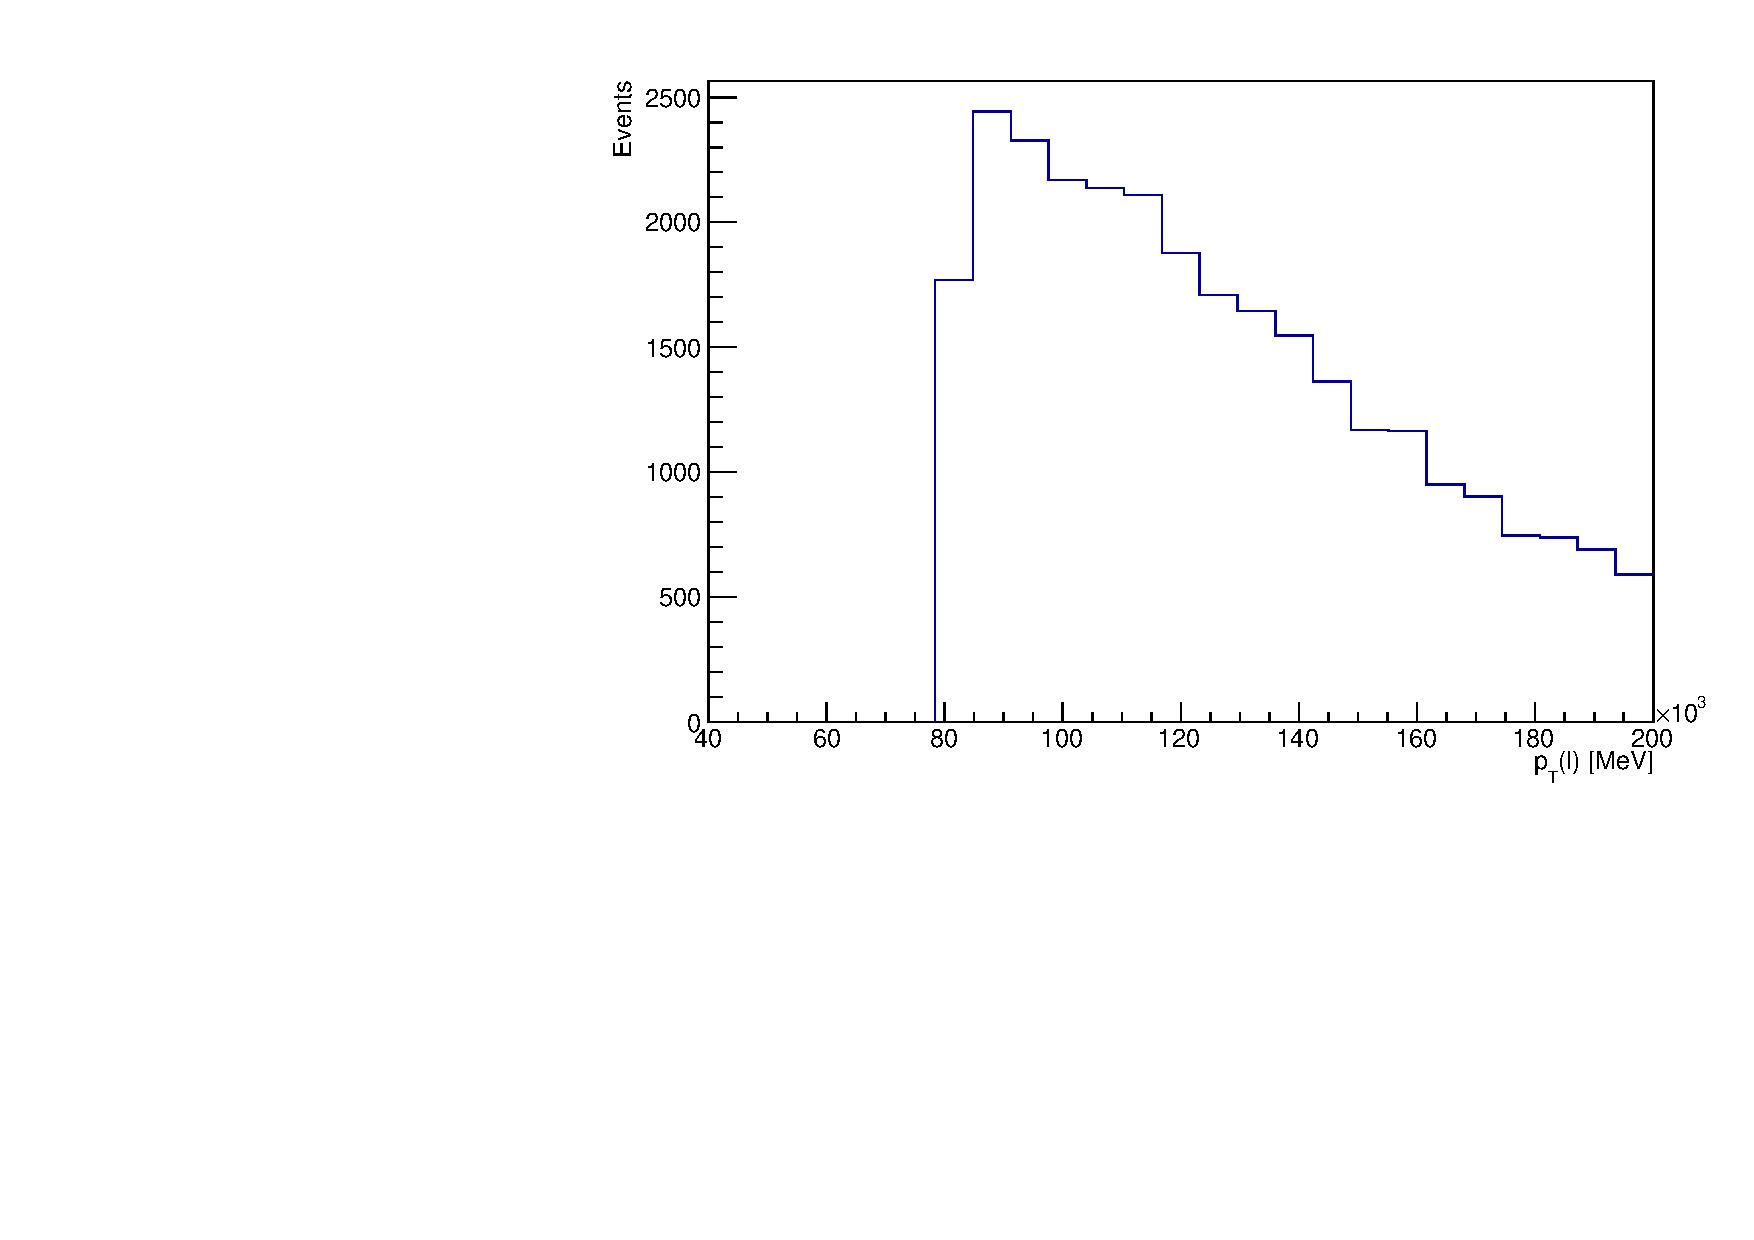
\includegraphics[width=\textwidth]{plots/ttbar_distributions/ttbar.mu_jet_pt_max.pdf}%
    \caption{Transverse momentum, lepton is muon.}%
    \label{fig:4b}%
  \end{subfigure}%

  \begin{subfigure}{0.45\textwidth}%
    \centering%
    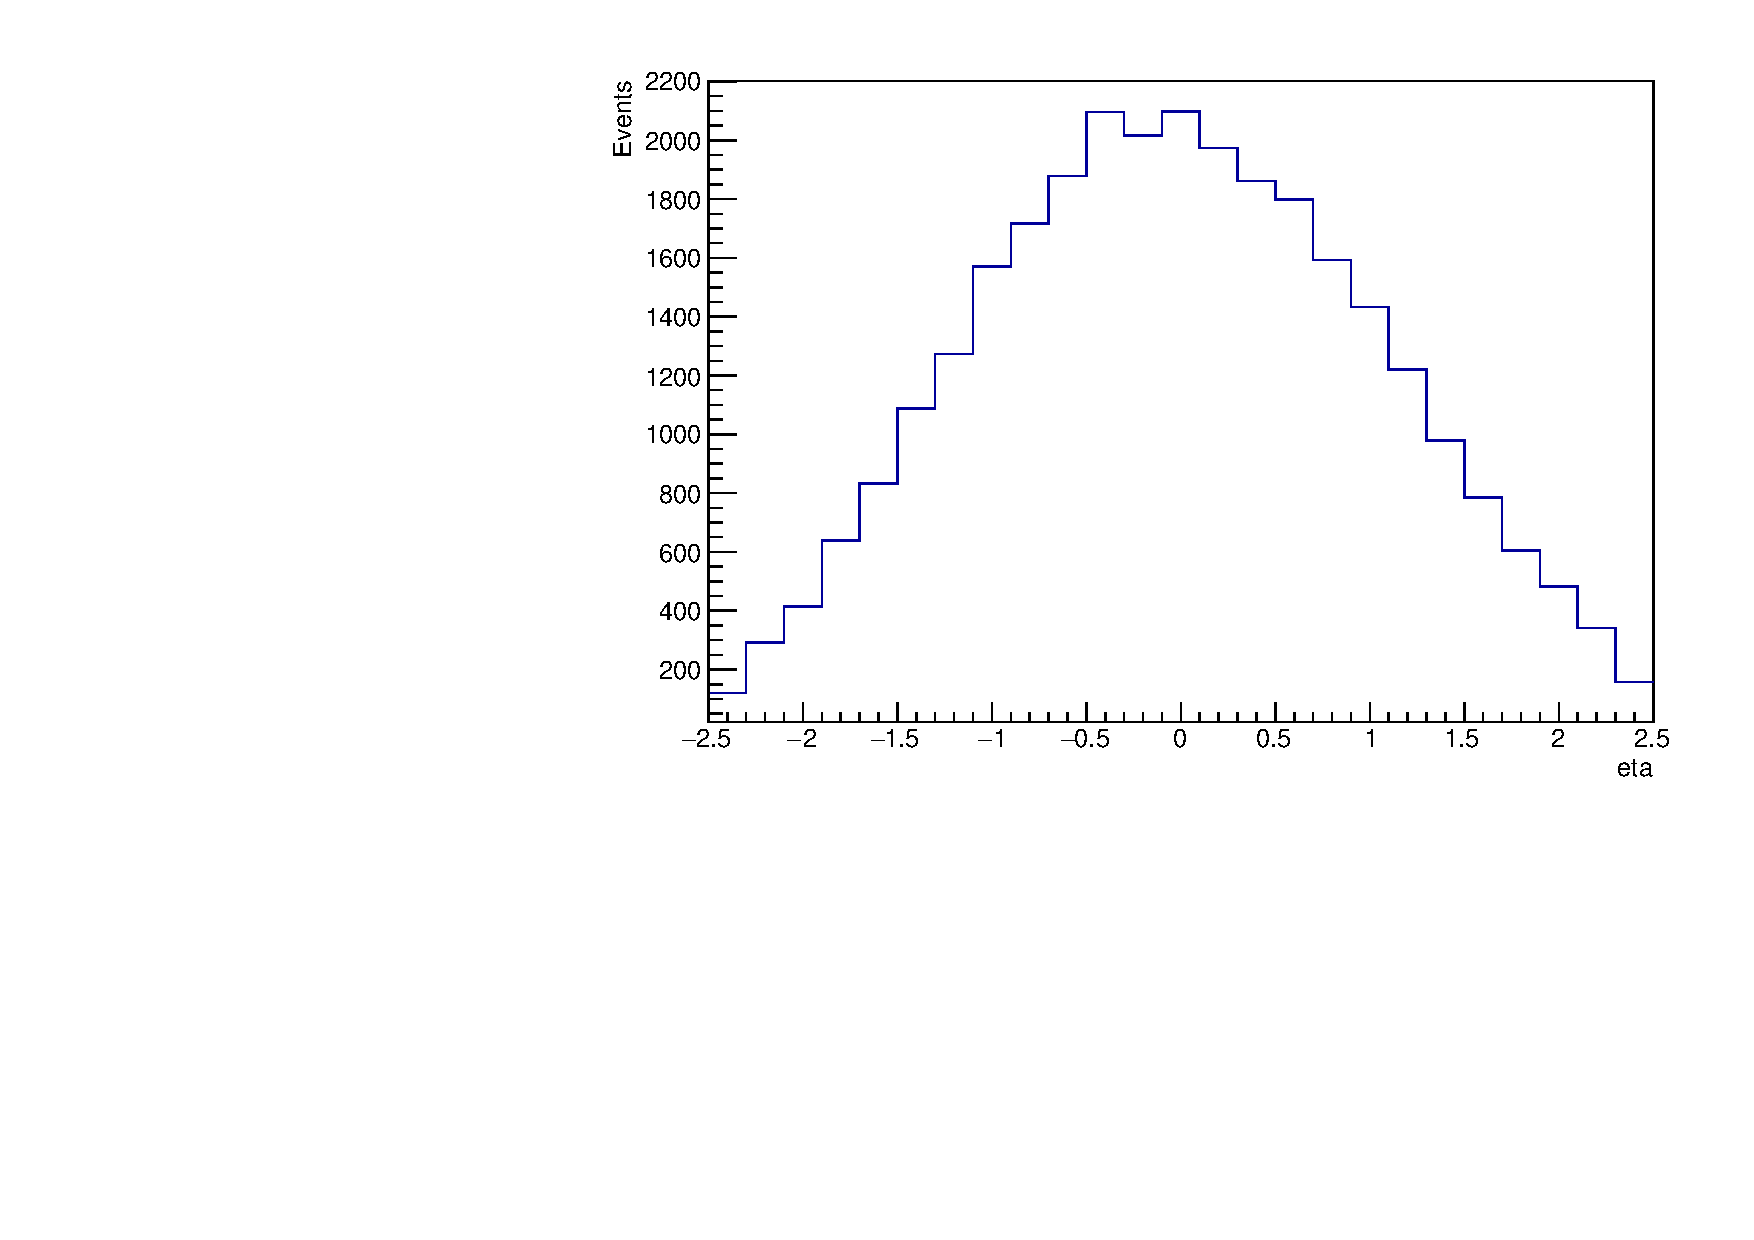
\includegraphics[width=\textwidth]{plots/ttbar_distributions/ttbar.el_jet_eta_max.pdf}%
    \caption{Pseudorapidity, lepton is electron.}%
    \label{fig:4c}%
  \end{subfigure}%
  \hfill
  \begin{subfigure}{0.45\textwidth}%
    \centering%
    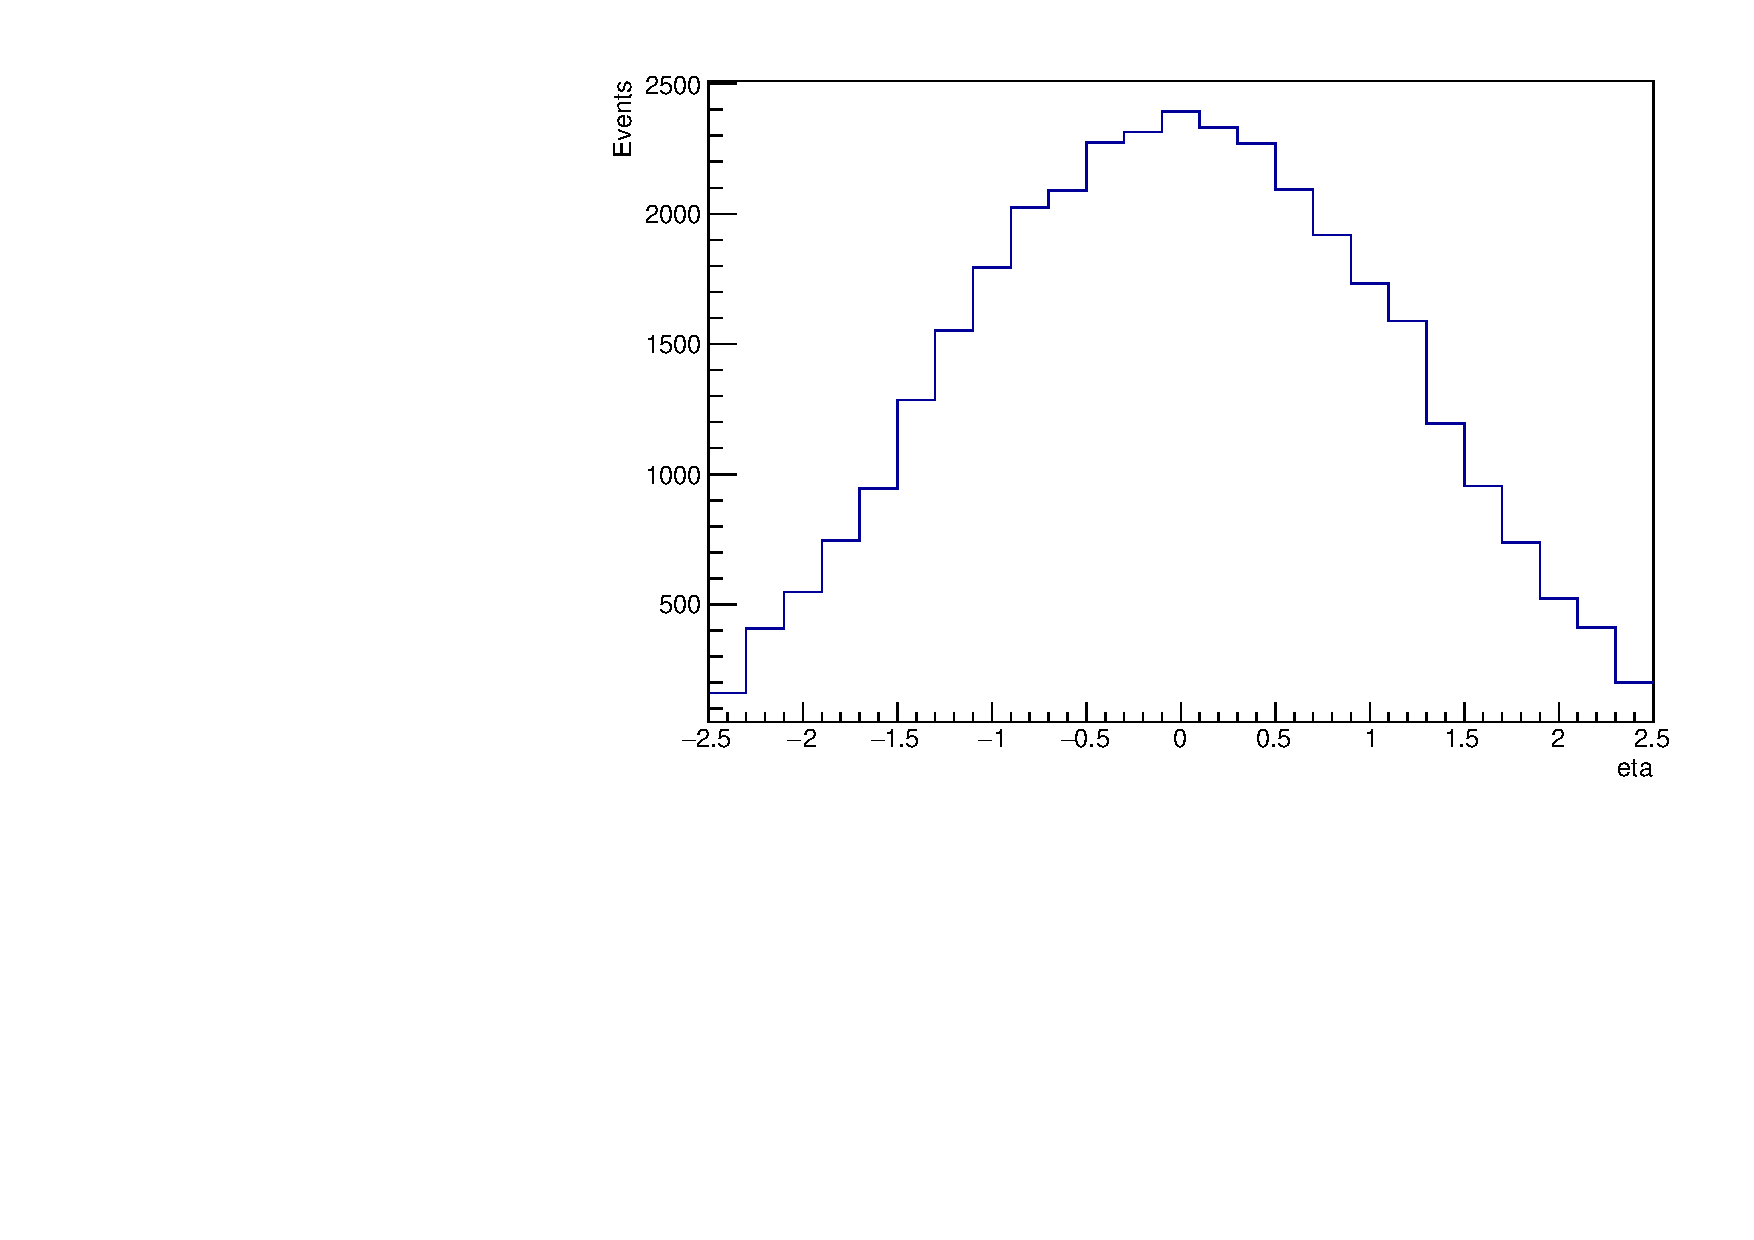
\includegraphics[width=\textwidth]{plots/ttbar_distributions/ttbar.mu_jet_eta_max.pdf}%
    \caption{Pseudorapidity, lepton is muon.}%
    \label{fig:4d}%
  \end{subfigure}%

  \begin{subfigure}{0.45\textwidth}%
    \centering%
    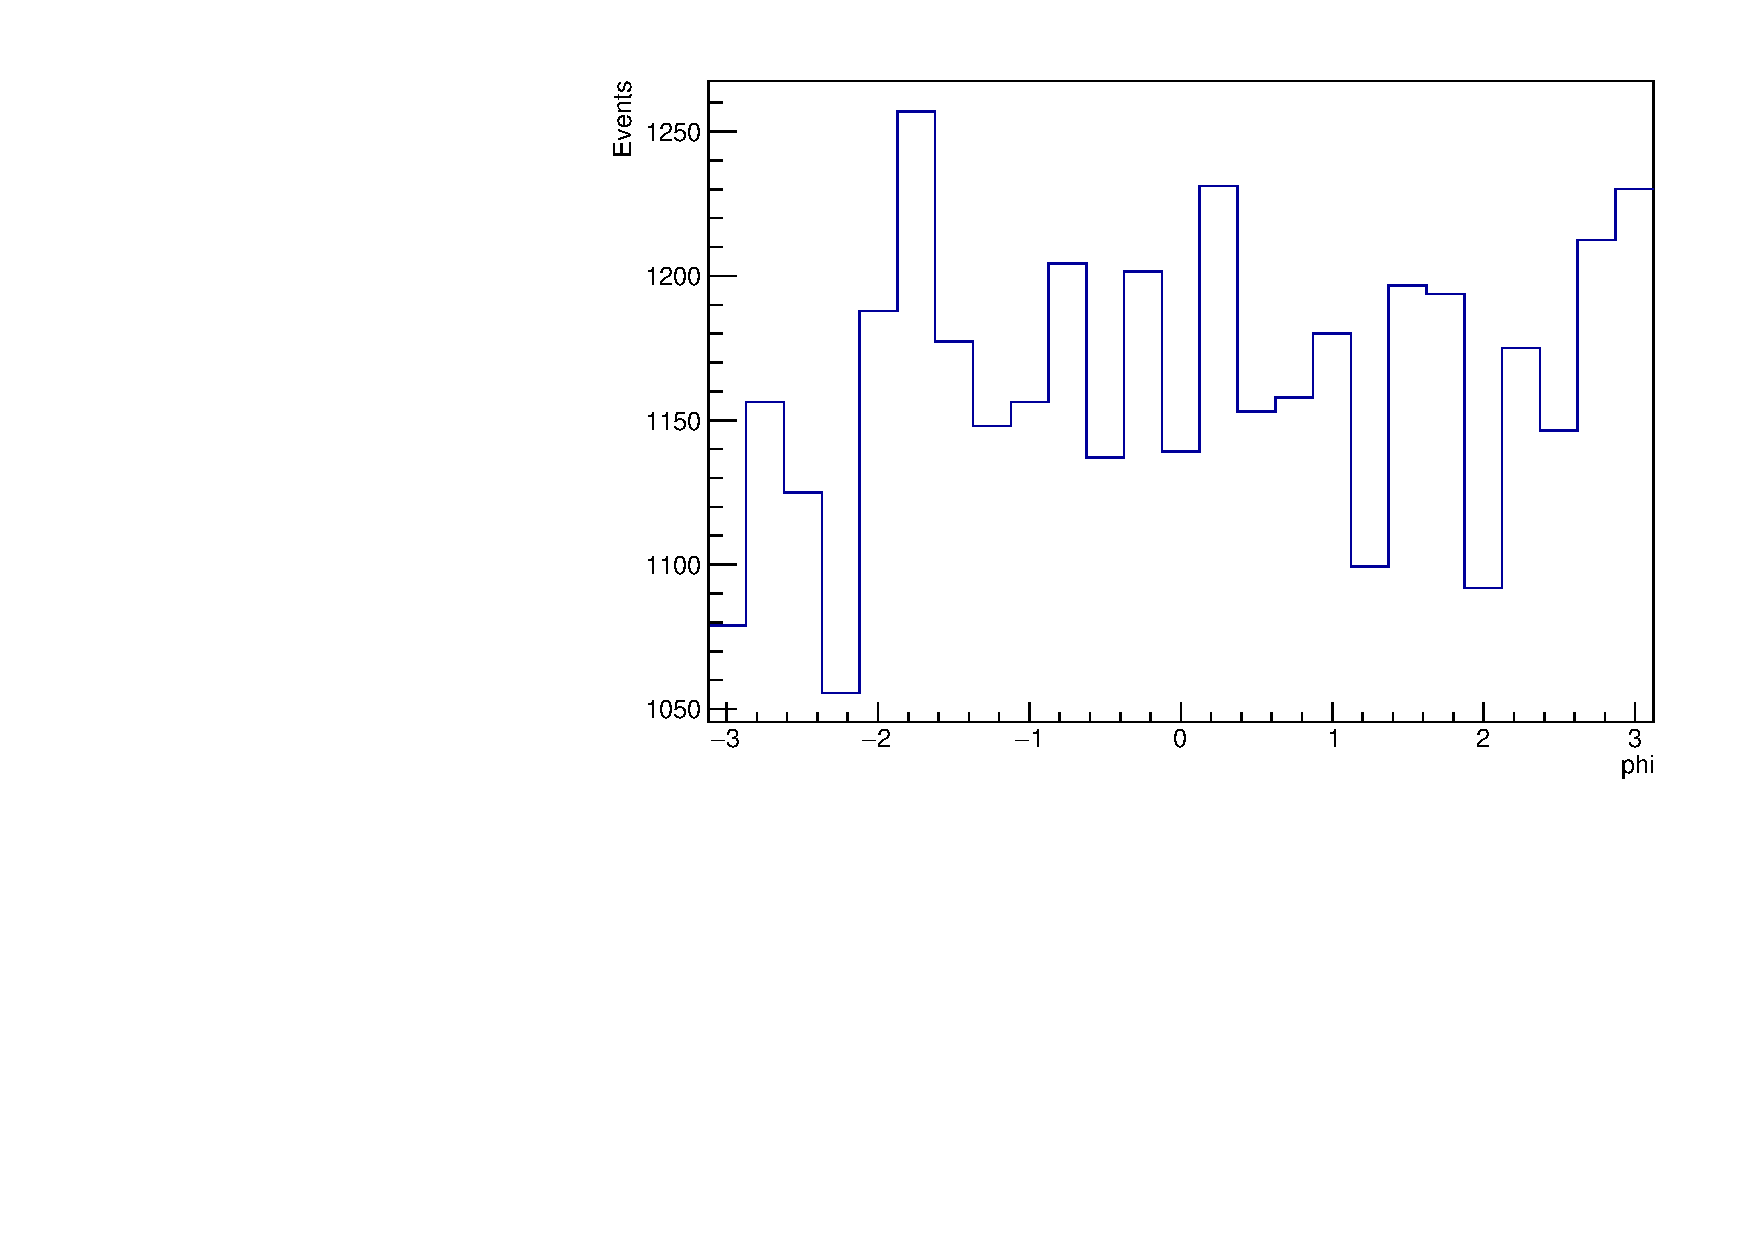
\includegraphics[width=\textwidth]{plots/ttbar_distributions/ttbar.el_jet_phi_max.pdf}%
    \caption{Polar angle, lepton is electron.}%
    \label{fig:4e}%
  \end{subfigure}%
  \hfill
  \begin{subfigure}{0.45\textwidth}%
    \centering%
    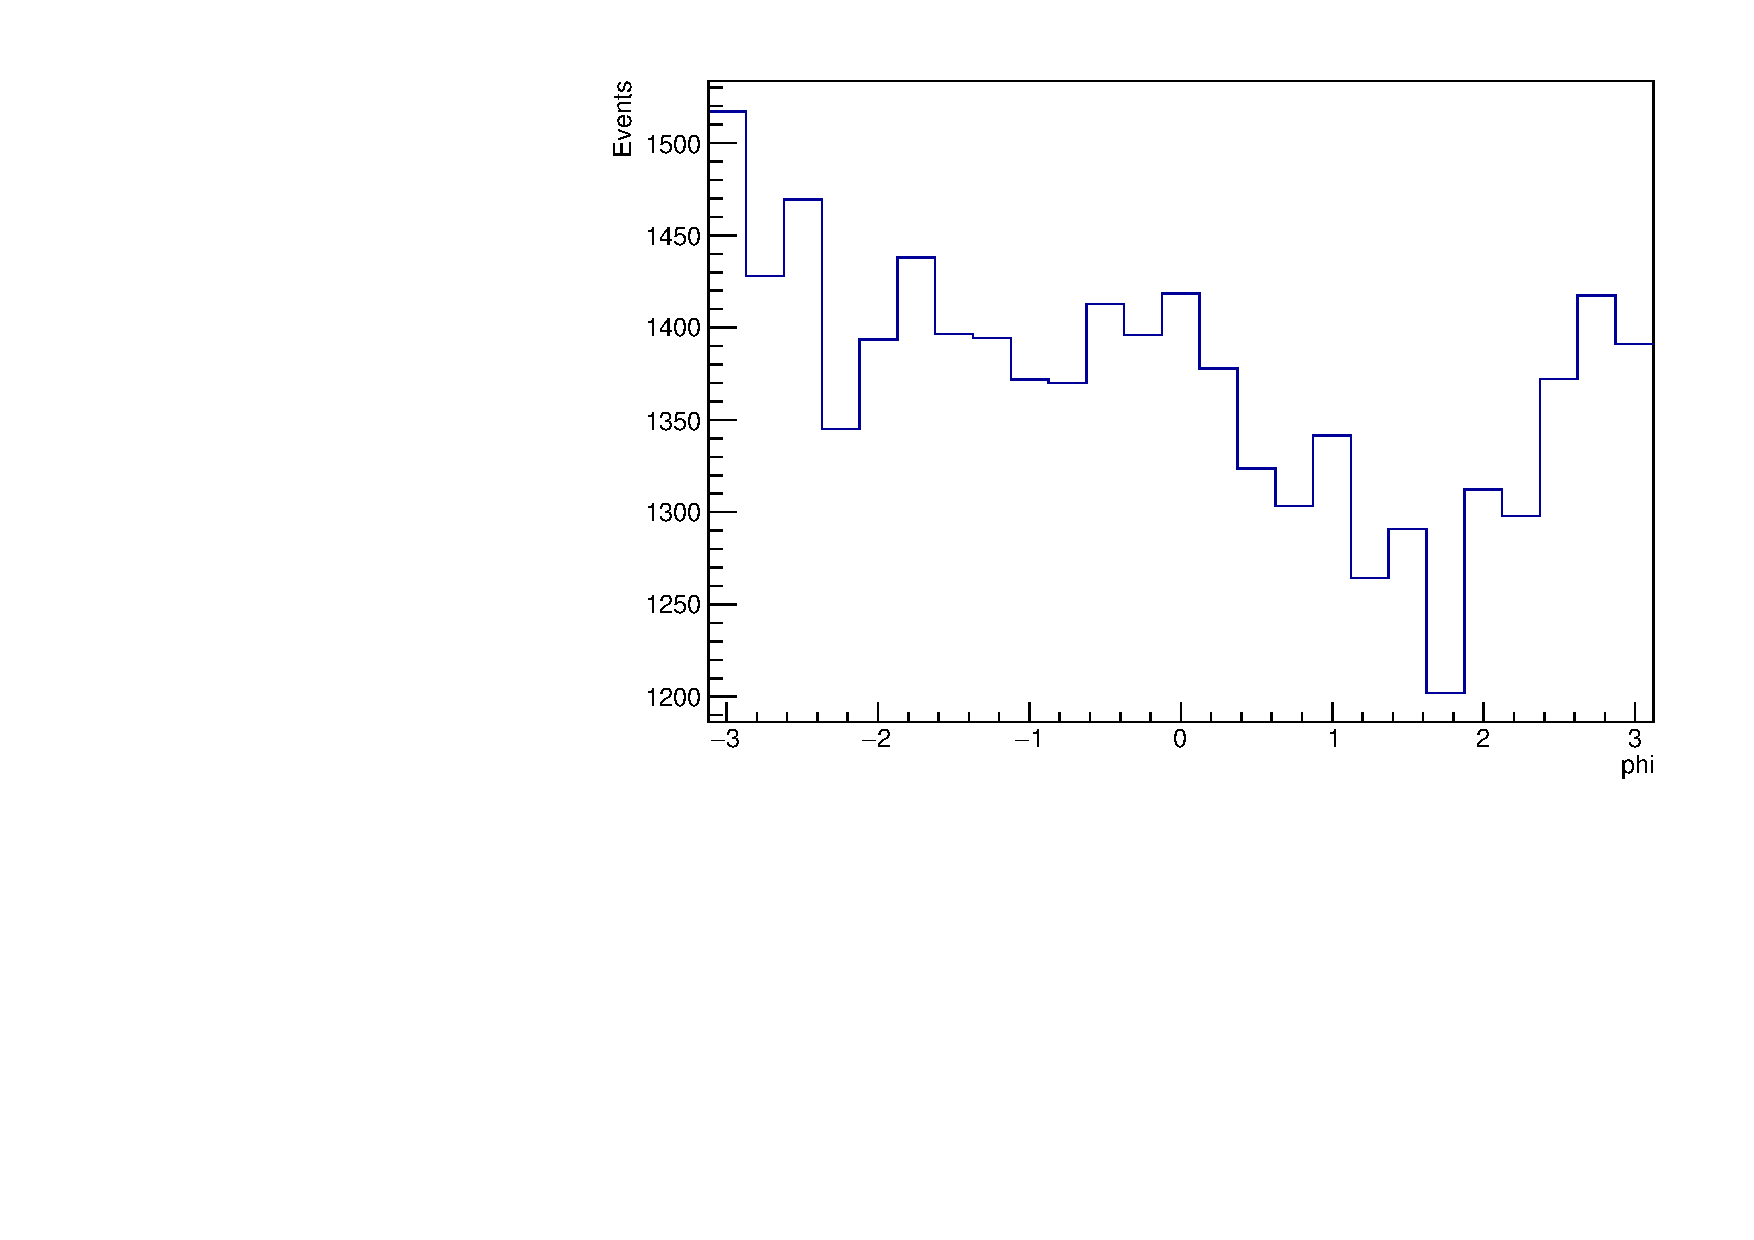
\includegraphics[width=\textwidth]{plots/ttbar_distributions/ttbar.mu_jet_phi_max.pdf}%
    \caption{Polar angle, lepton is muon.}%
    \label{fig:4f}%
  \end{subfigure}%

  \begin{subfigure}{0.45\textwidth}%
    \centering%
    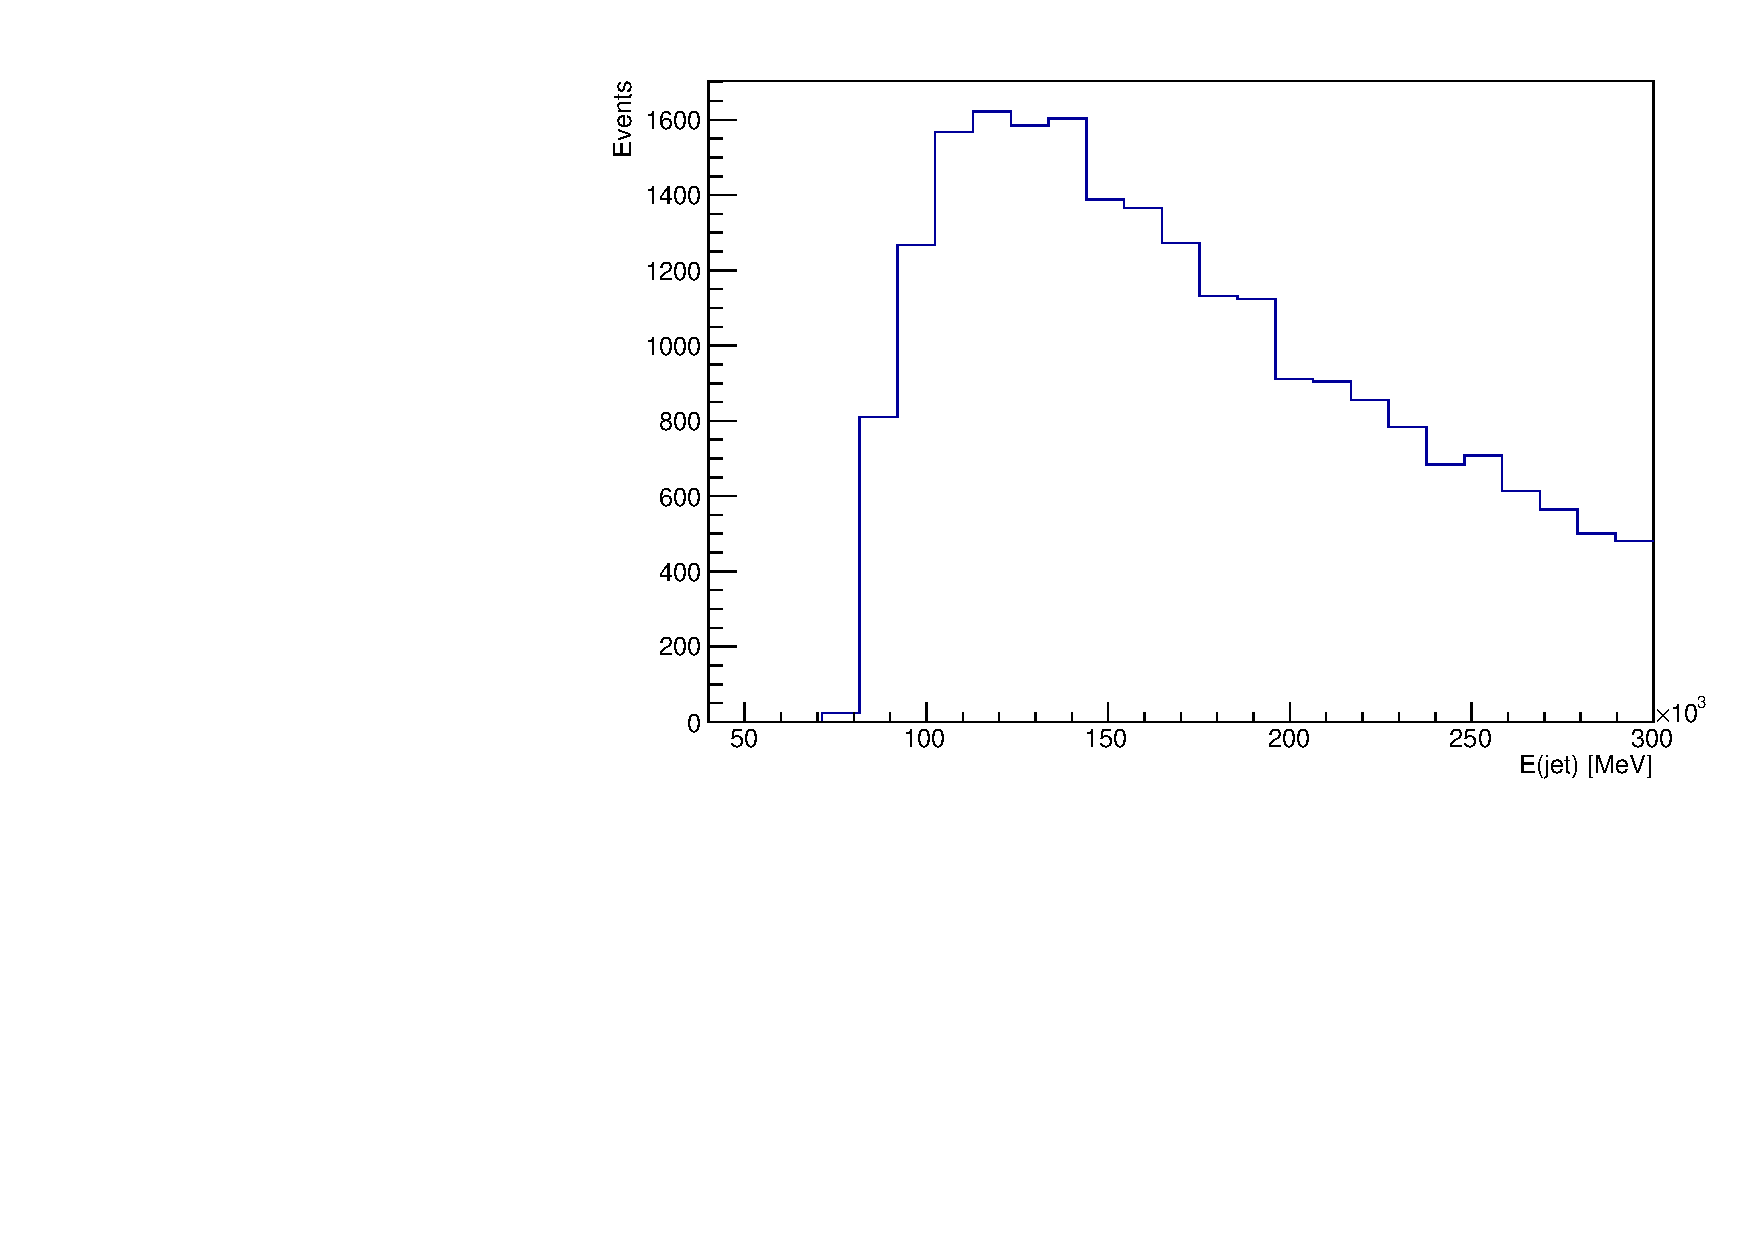
\includegraphics[width=\textwidth]{plots/ttbar_distributions/ttbar.el_jet_E_max.pdf}%
    \caption{Energy, lepton is electron.}%
    \label{fig:4g}%
  \end{subfigure}%
  \hfill
  \begin{subfigure}{0.45\textwidth}%
    \centering%
    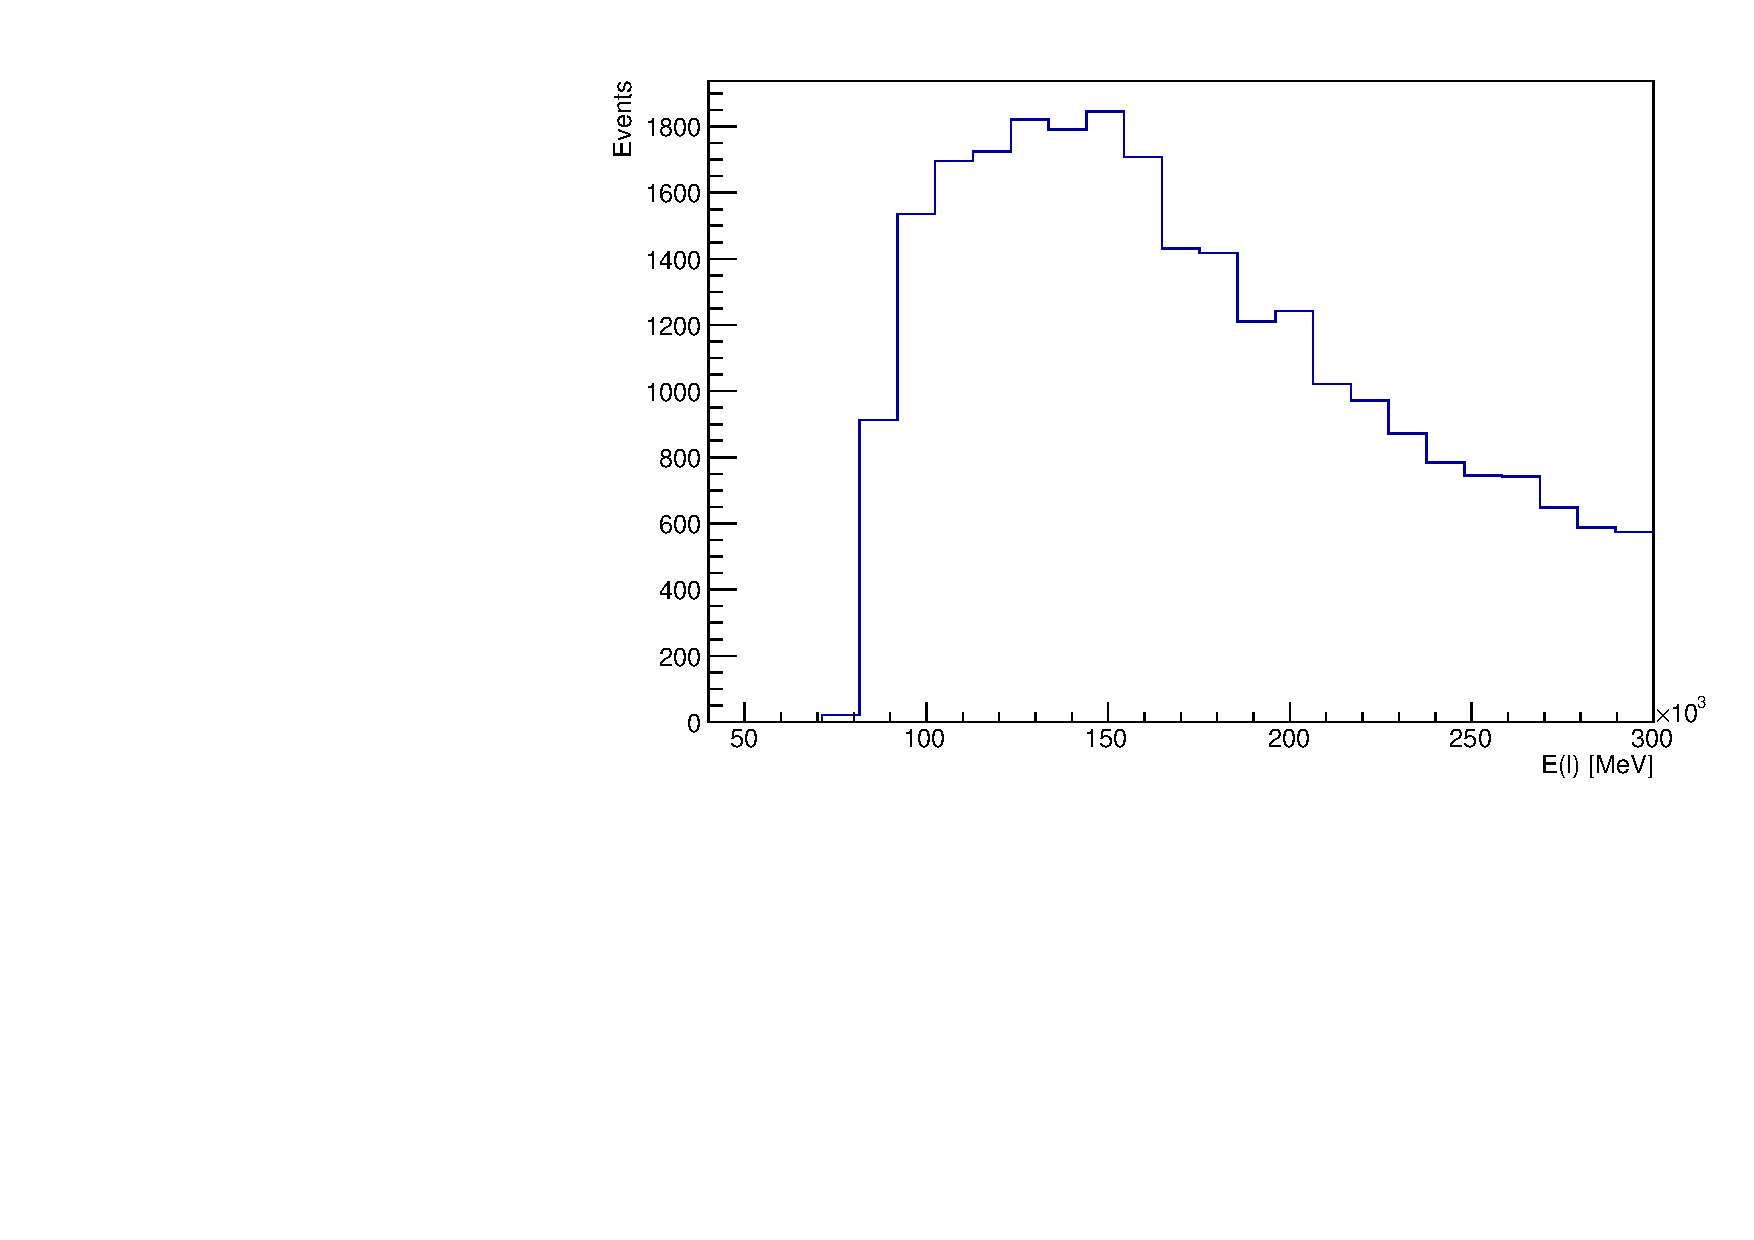
\includegraphics[width=\textwidth]{plots/ttbar_distributions/ttbar.mu_jet_E_max.pdf}%
    \caption{Energy, lepton is muon.}%
    \label{fig:4h}%
  \end{subfigure}%
  \caption{Histograms of the parameters for the jet with the maximal transverse momentum for each event.}%
  \label{fig:4}%
\end{figure}

\subsection{Discriminant}
To further improve signal to backgroud ratio of the samples discriminants constructed from the four vectors of the particles in the events are investigated. 
Specifically 
\begin{itemize}
  \item the missing transverse momentum (dis 1),
  \item the difference of the azimuthal angle between the missing transverse momentum and the lepton (dis. 2), 
  \item the invariant mass of system formed by the three jets with the maximal transverse momentum (dis. 3),
  \item the invariant mass of system formed by the four jets with the maximal transverse momentum, the lepton and the missing transverse momentum (dis. 4), 
  \item the pseudorapidity of system formed by the four jets with the maximal transverse momentum, the lepton and the missing transverse momentum (dis.5) 
\end{itemize}
are considered and histograms are created for simulated $t \overline{t}$- and $Z^\prime(1 \, \si{\giga\eV})$-events. Those histograms are shown in figure 
\ref{fig:5} and figure \ref{fig:6}.


\begin{figure}[H]%
  \begin{subfigure}{0.48\textwidth}%
    \centering%
    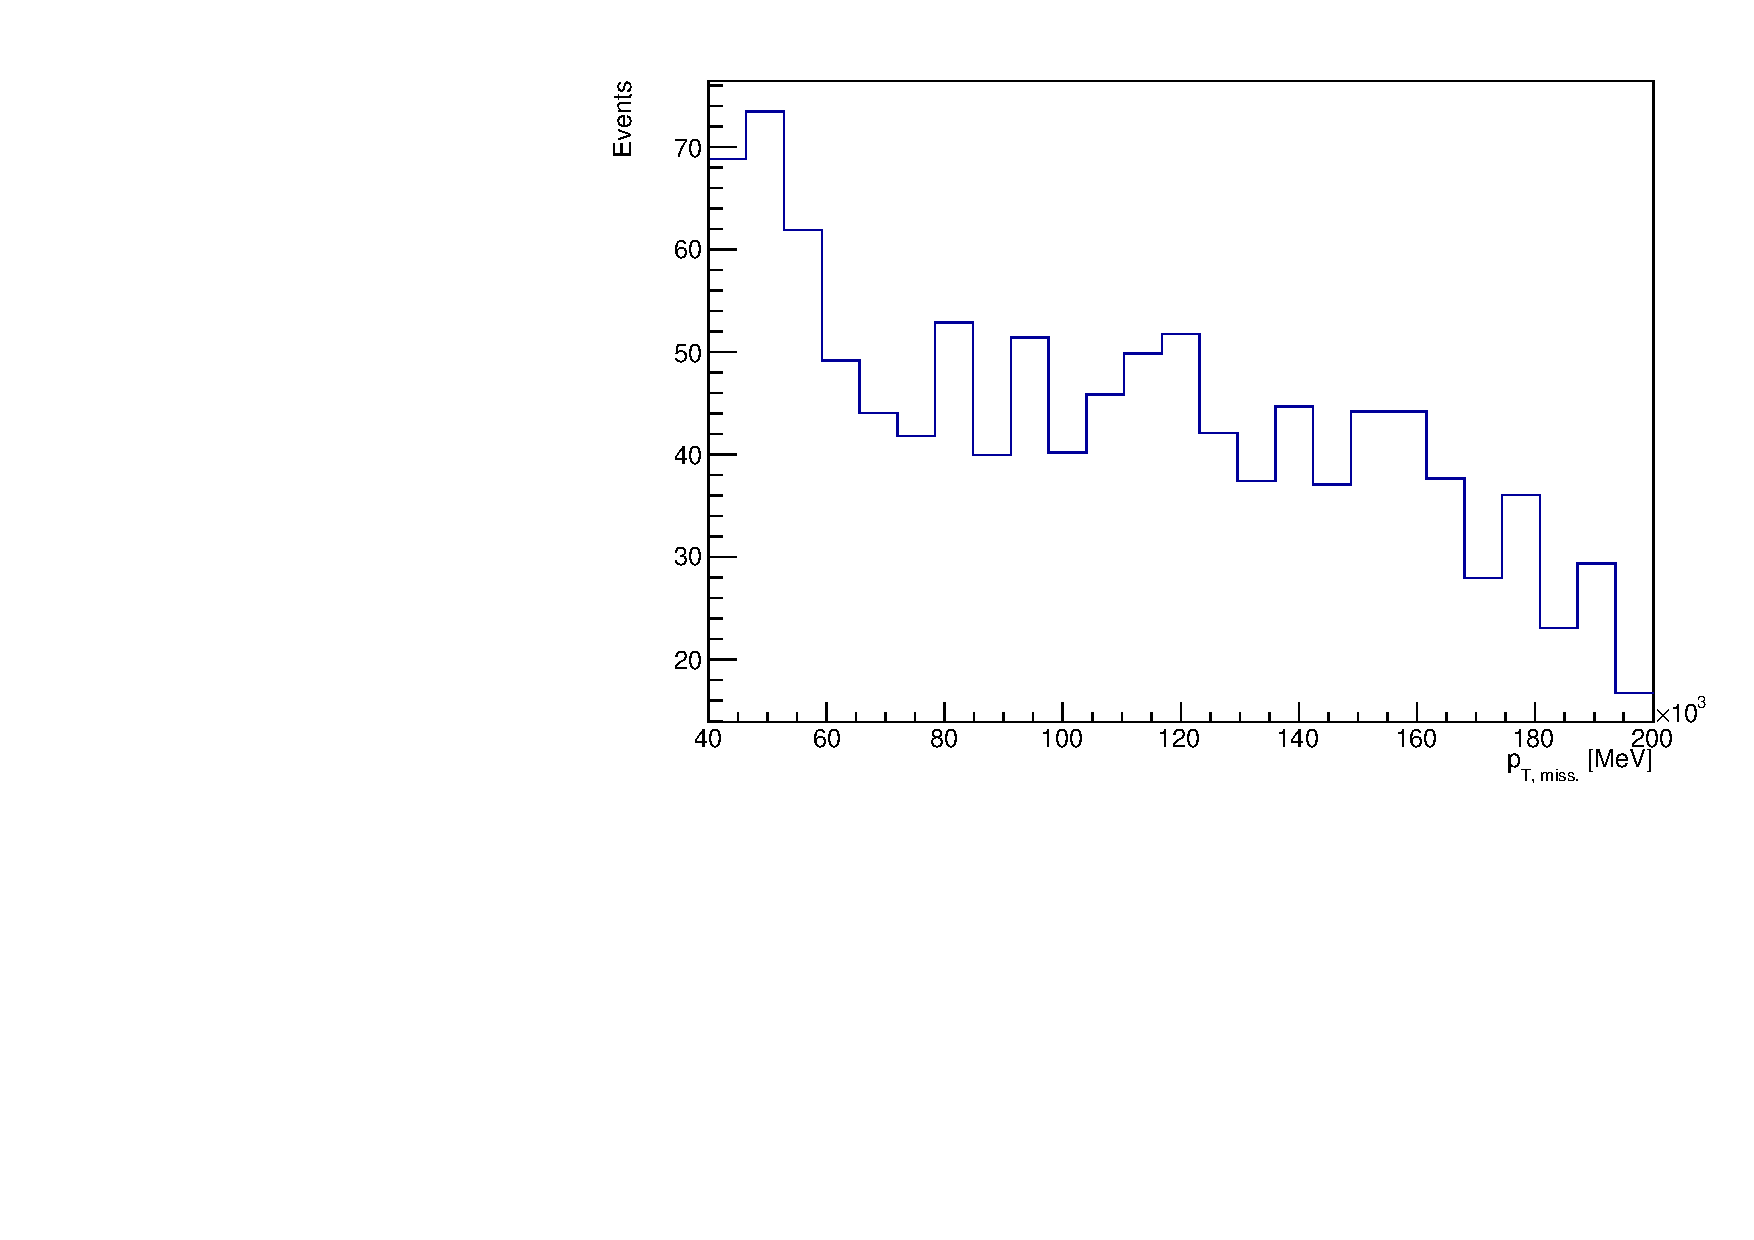
\includegraphics[width=\textwidth]{plots/discriminant/zprime1000.el_met_et.pdf}%
    \caption{dis. 1, $Z^\prime(1000 \, \si{\giga\eV})$}%
    \label{fig:5a}%
  \end{subfigure}%
  \hfill
  \begin{subfigure}{0.48\textwidth}%
    \centering%
    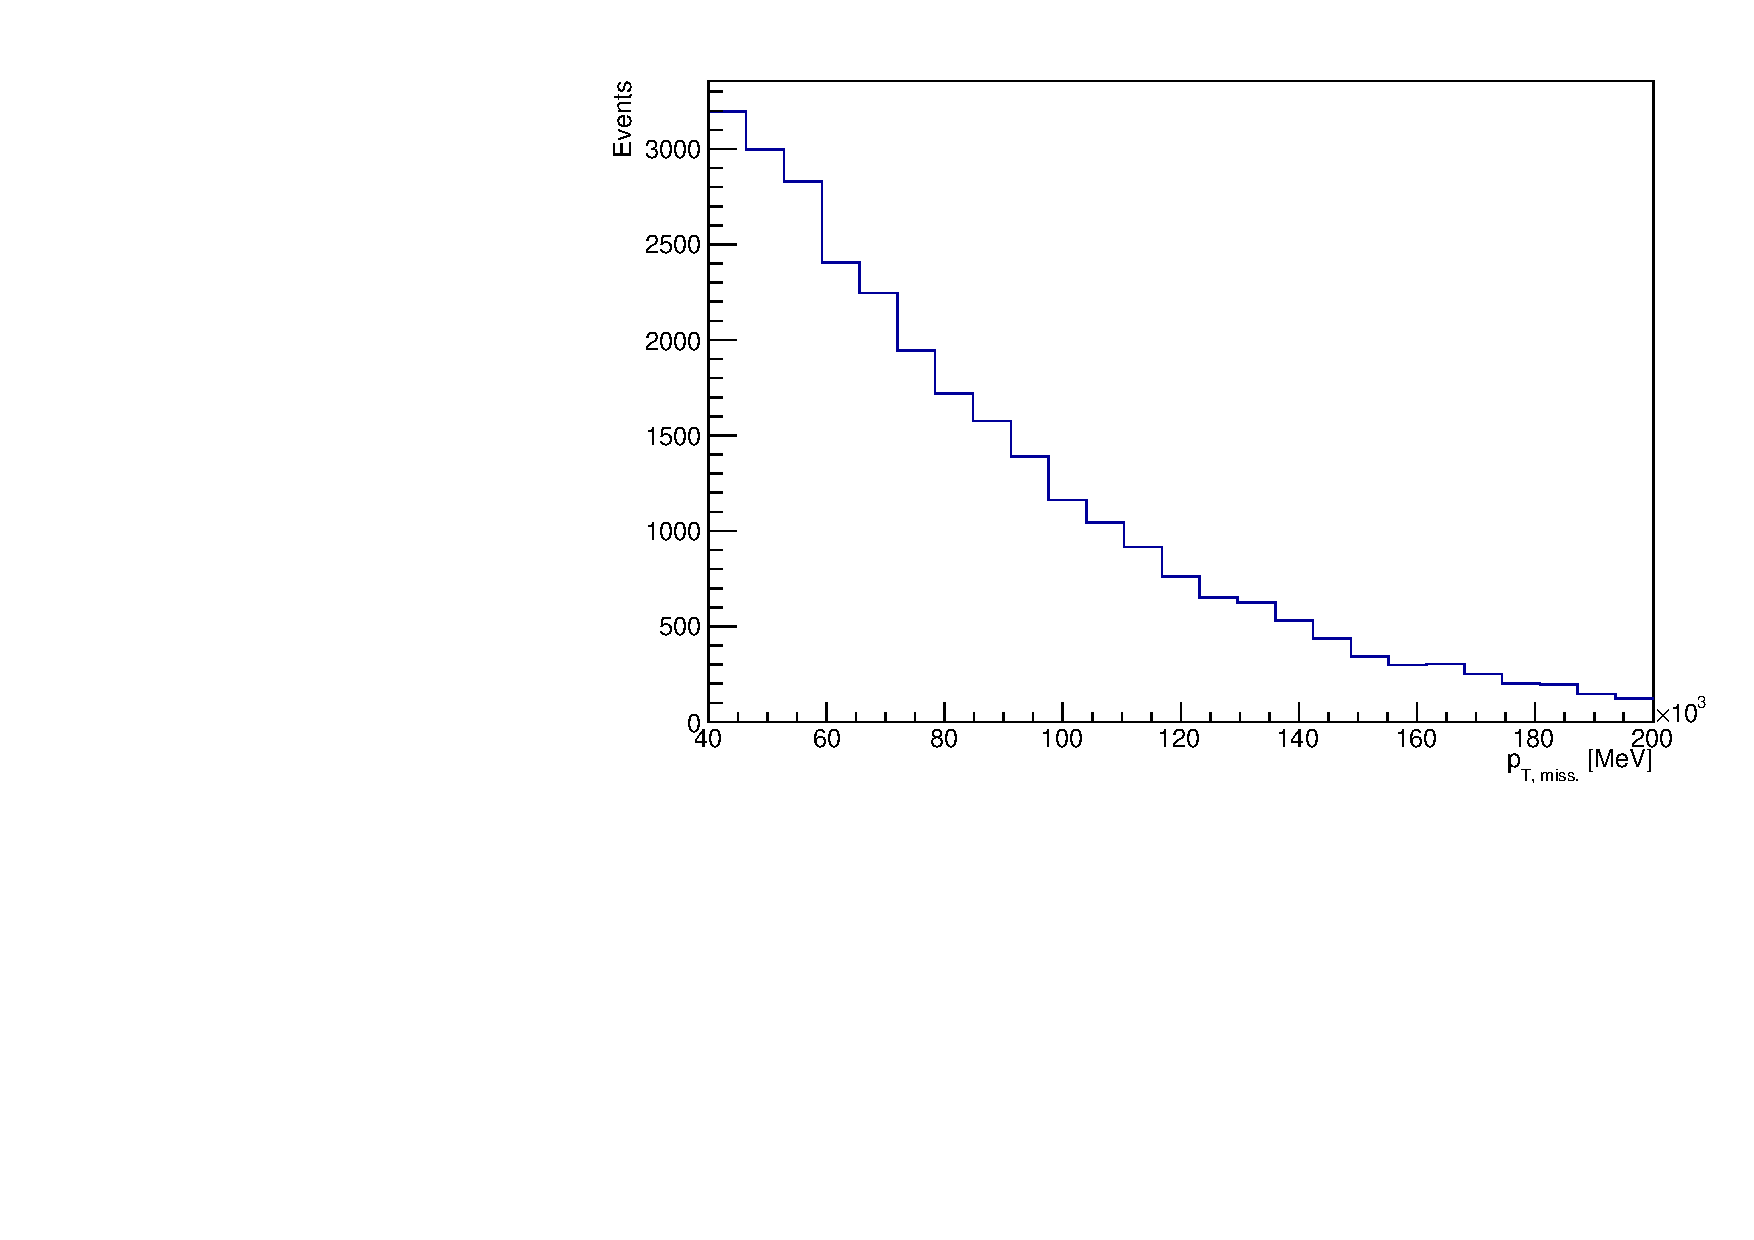
\includegraphics[width=\textwidth]{plots/discriminant/ttbar.el_met_et.pdf}%
    \caption{dis. 1, $t \overline{t}$}%
    \label{fig:5b}%
  \end{subfigure}%

  \begin{subfigure}{0.45\textwidth}%
    \centering%
    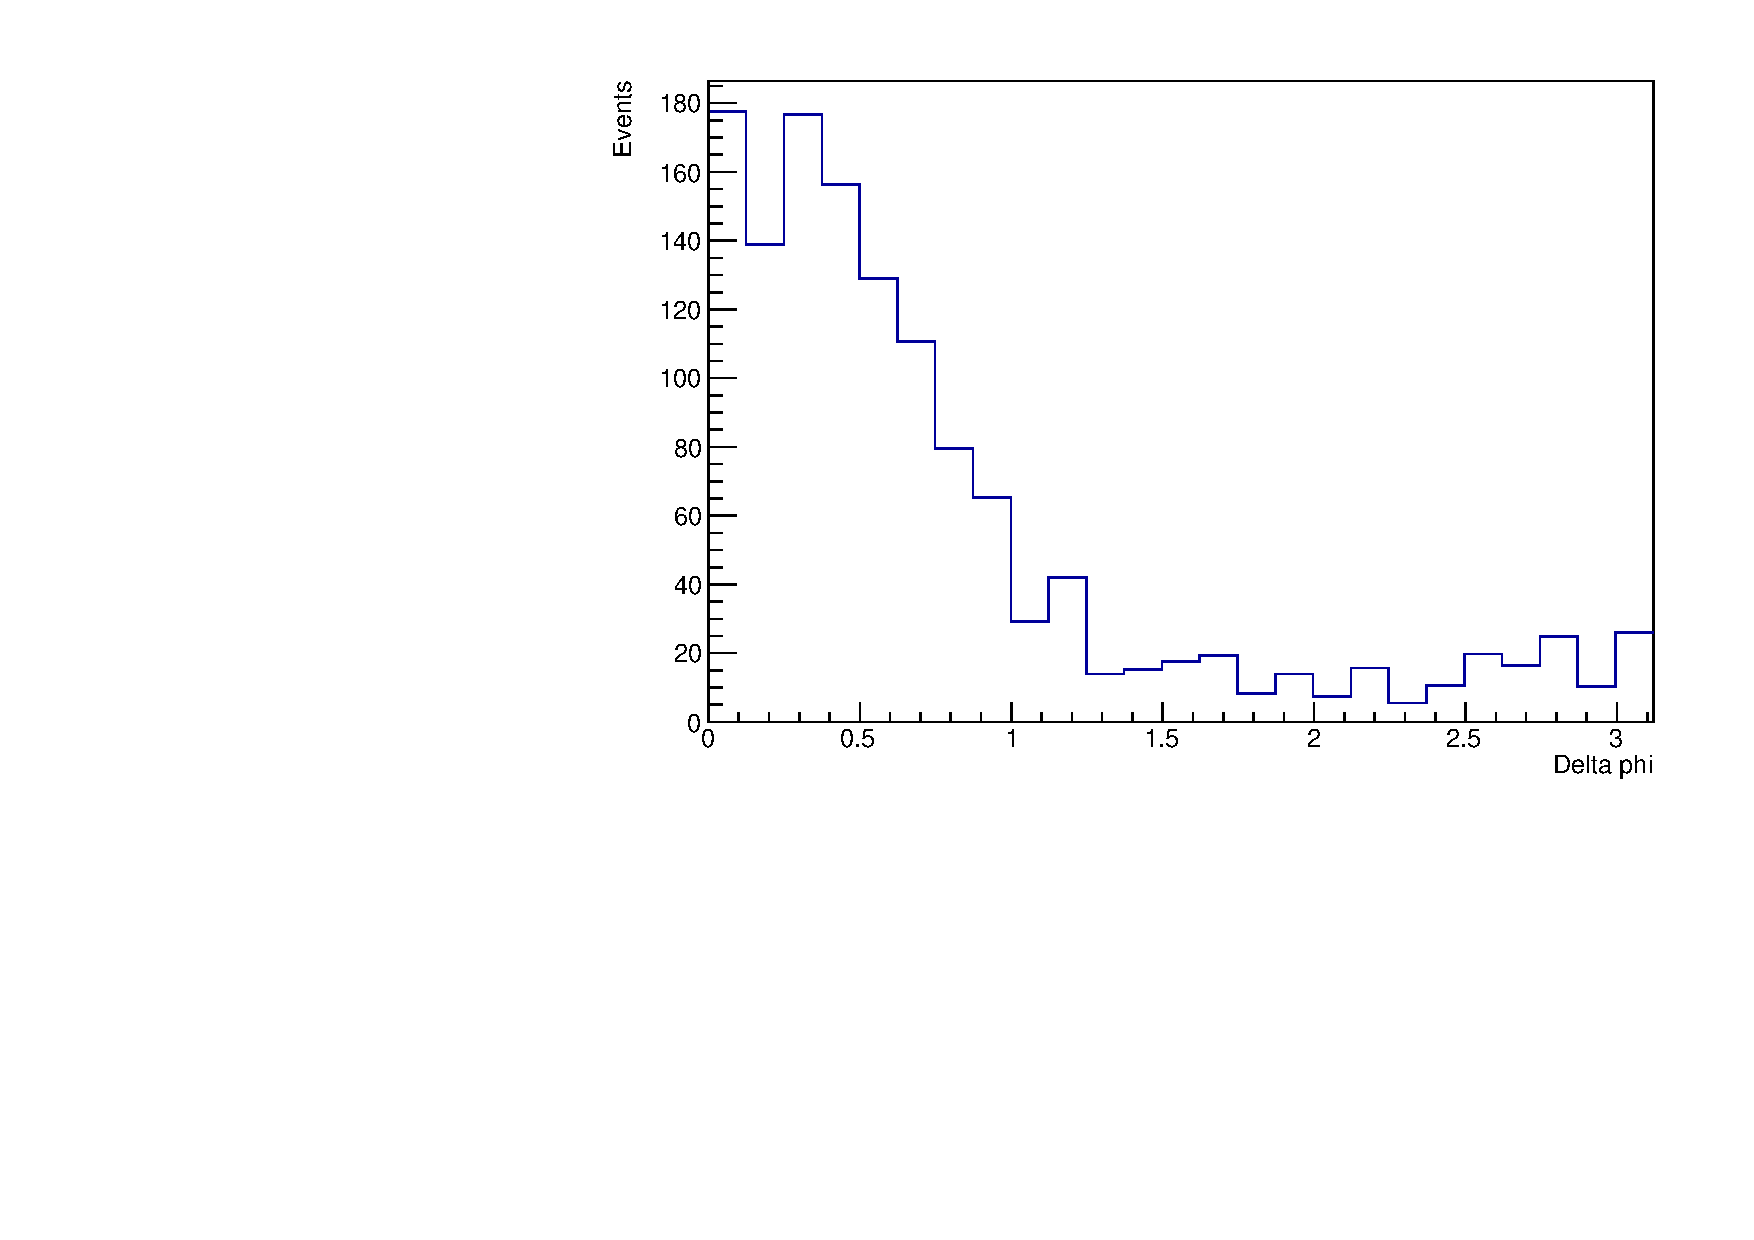
\includegraphics[width=\textwidth]{plots/discriminant/zprime1000.el_del_phi.pdf}%
    \caption{dis. 2, $Z^\prime(1000 \, \si{\giga\eV})$}%
    \label{fig:5c}%
  \end{subfigure}%
  \hfill
  \begin{subfigure}{0.45\textwidth}%
    \centering%
    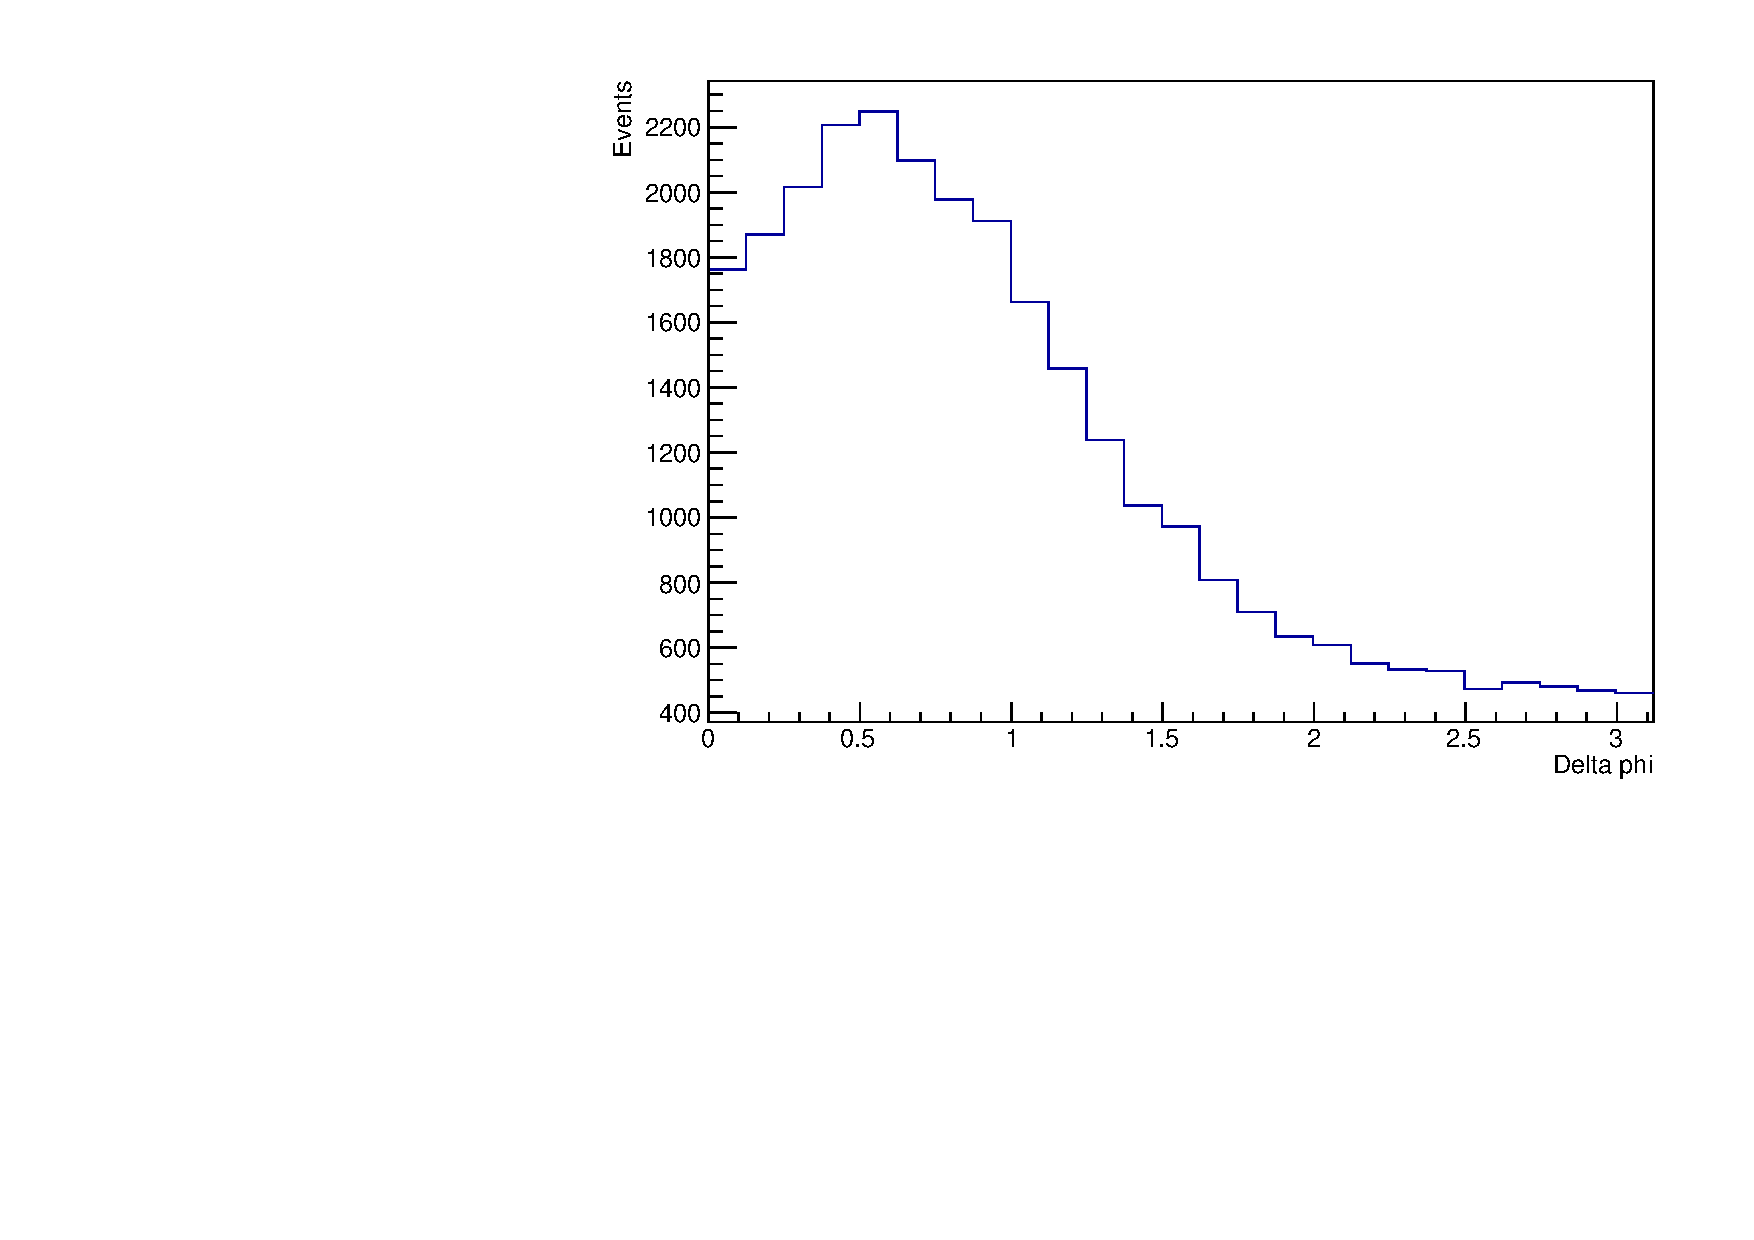
\includegraphics[width=\textwidth]{plots/discriminant/ttbar.el_del_phi.pdf}%
    \caption{dis. 2, $t \overline{t}$}%
    \label{fig:5d}%
  \end{subfigure}%

  \begin{subfigure}{0.45\textwidth}%
    \centering%
    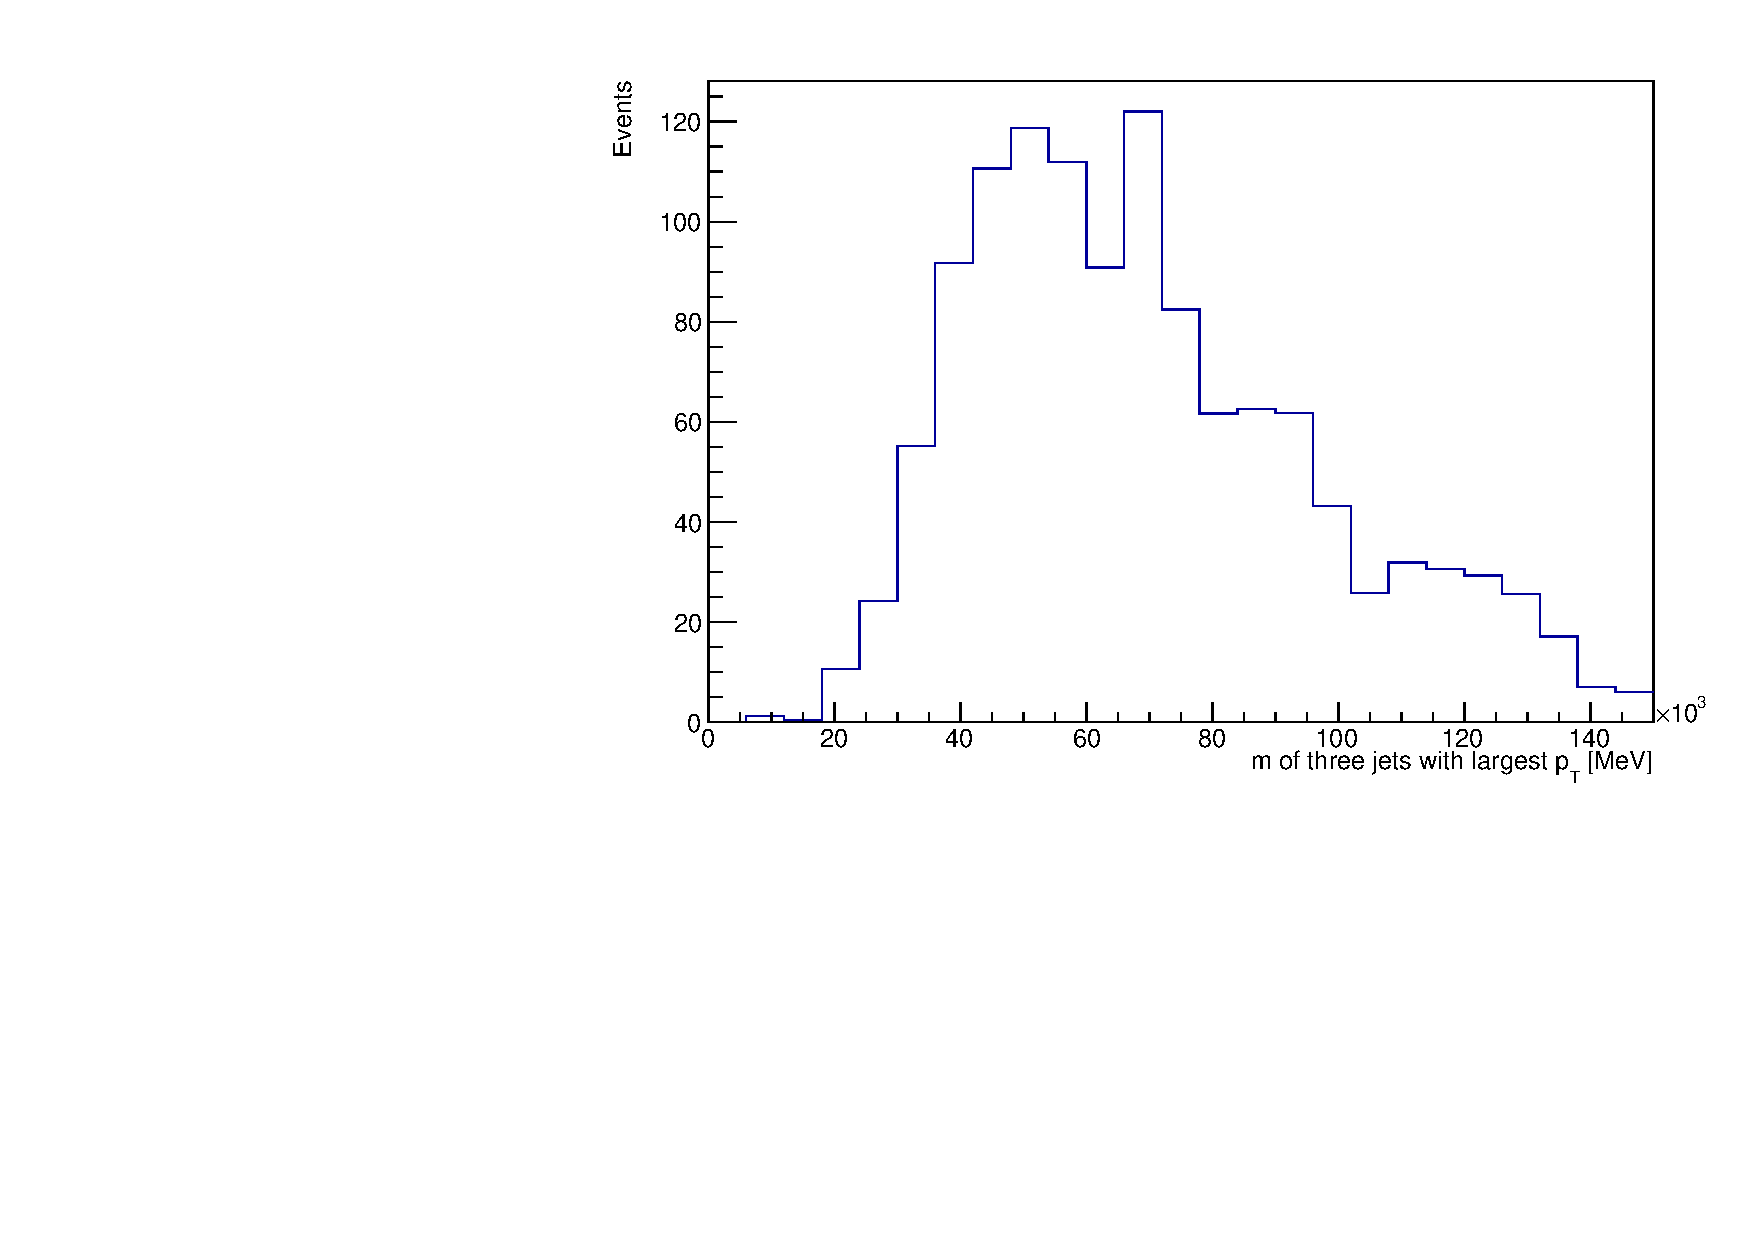
\includegraphics[width=\textwidth]{plots/discriminant/zprime1000.el_dis3.pdf}%
    \caption{dis. 3, $Z^\prime(1000 \, \si{\giga\eV})$}%
    \label{fig:5e}%
  \end{subfigure}%
  \hfill
  \begin{subfigure}{0.45\textwidth}%
    \centering%
    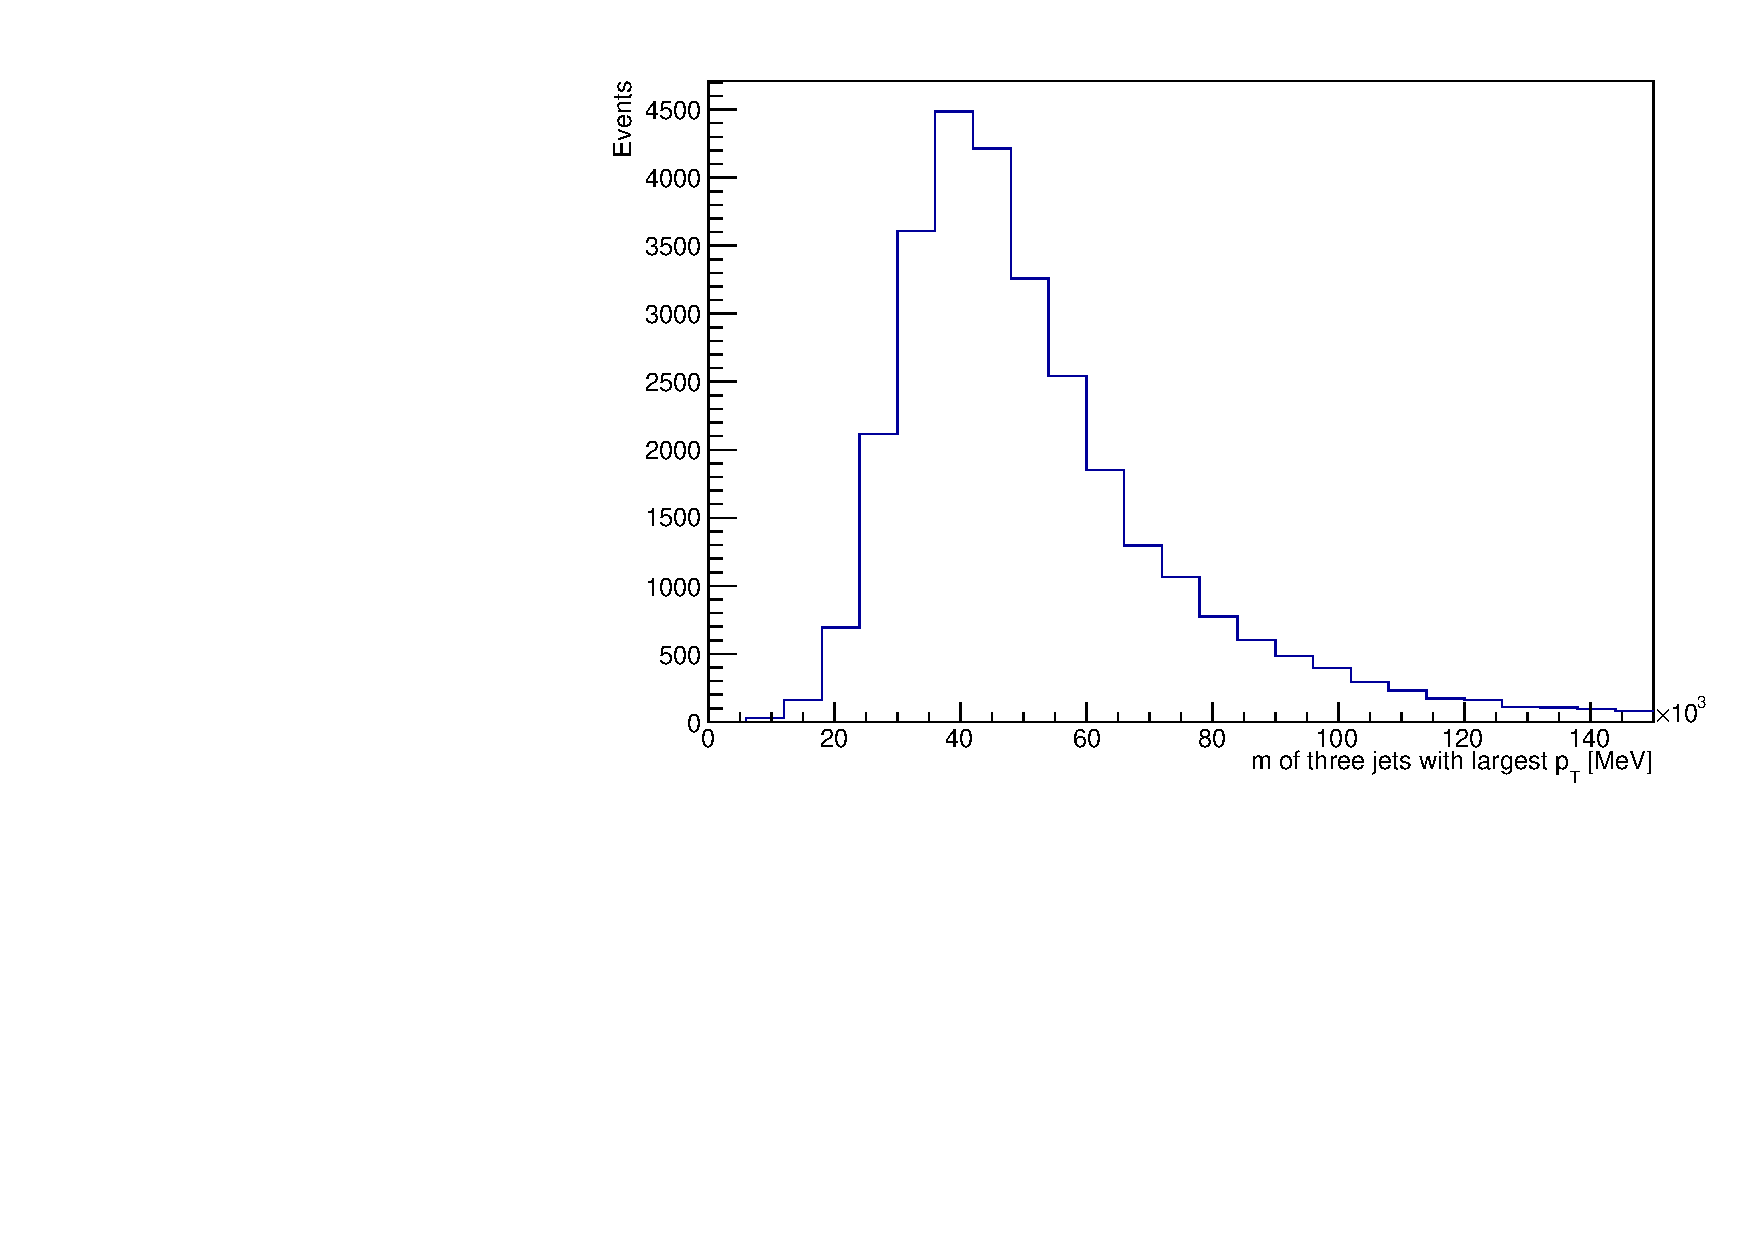
\includegraphics[width=\textwidth]{plots/discriminant/ttbar.el_dis3.pdf}%
    \caption{dis. 3, $t \overline{t}$}%
    \label{fig:5f}%
  \end{subfigure}%

  \begin{subfigure}{0.45\textwidth}%
    \centering%
    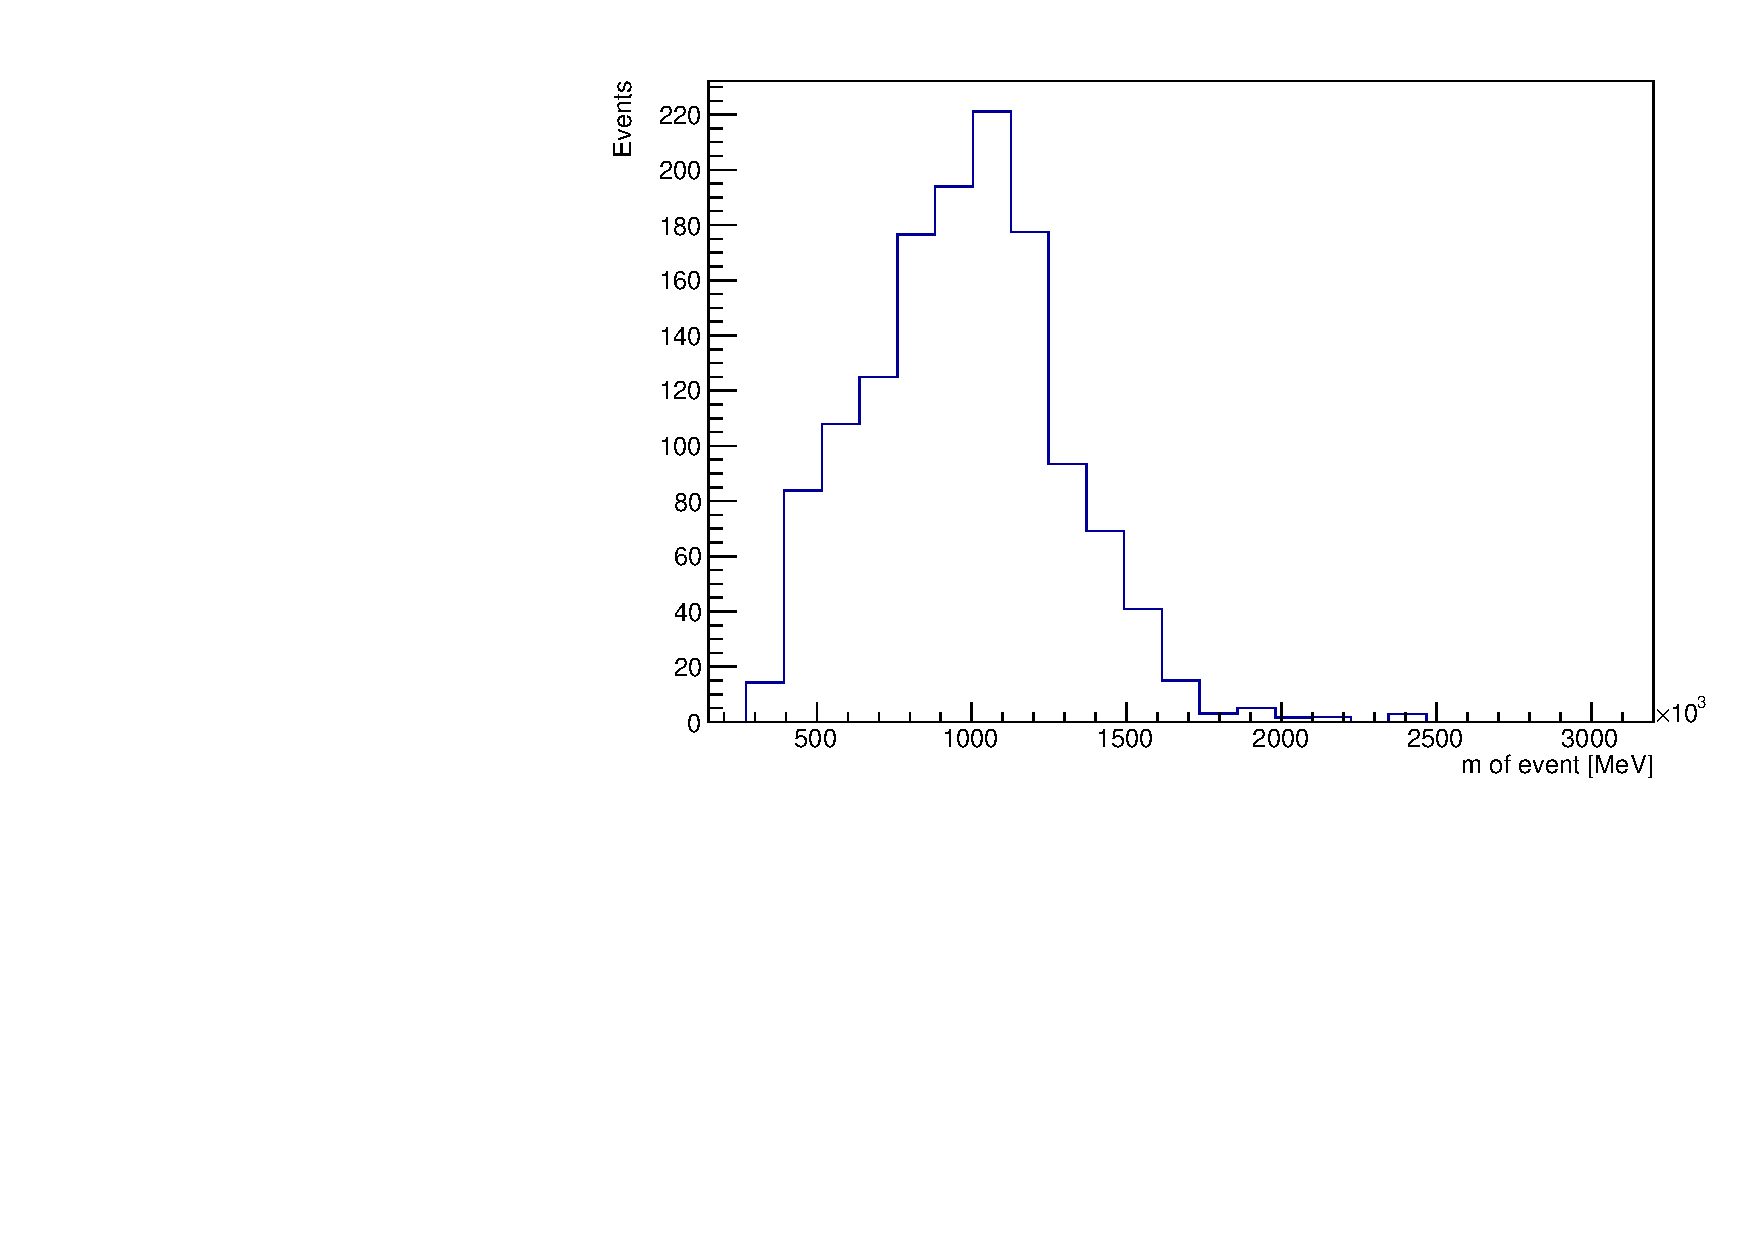
\includegraphics[width=\textwidth]{plots/discriminant/zprime1000.el_dis4.pdf}%
    \caption{dis. 4, $Z^\prime(1000 \, \si{\giga\eV})$}%
    \label{fig:5g}%
  \end{subfigure}%
  \hfill
  \begin{subfigure}{0.45\textwidth}%
    \centering%
    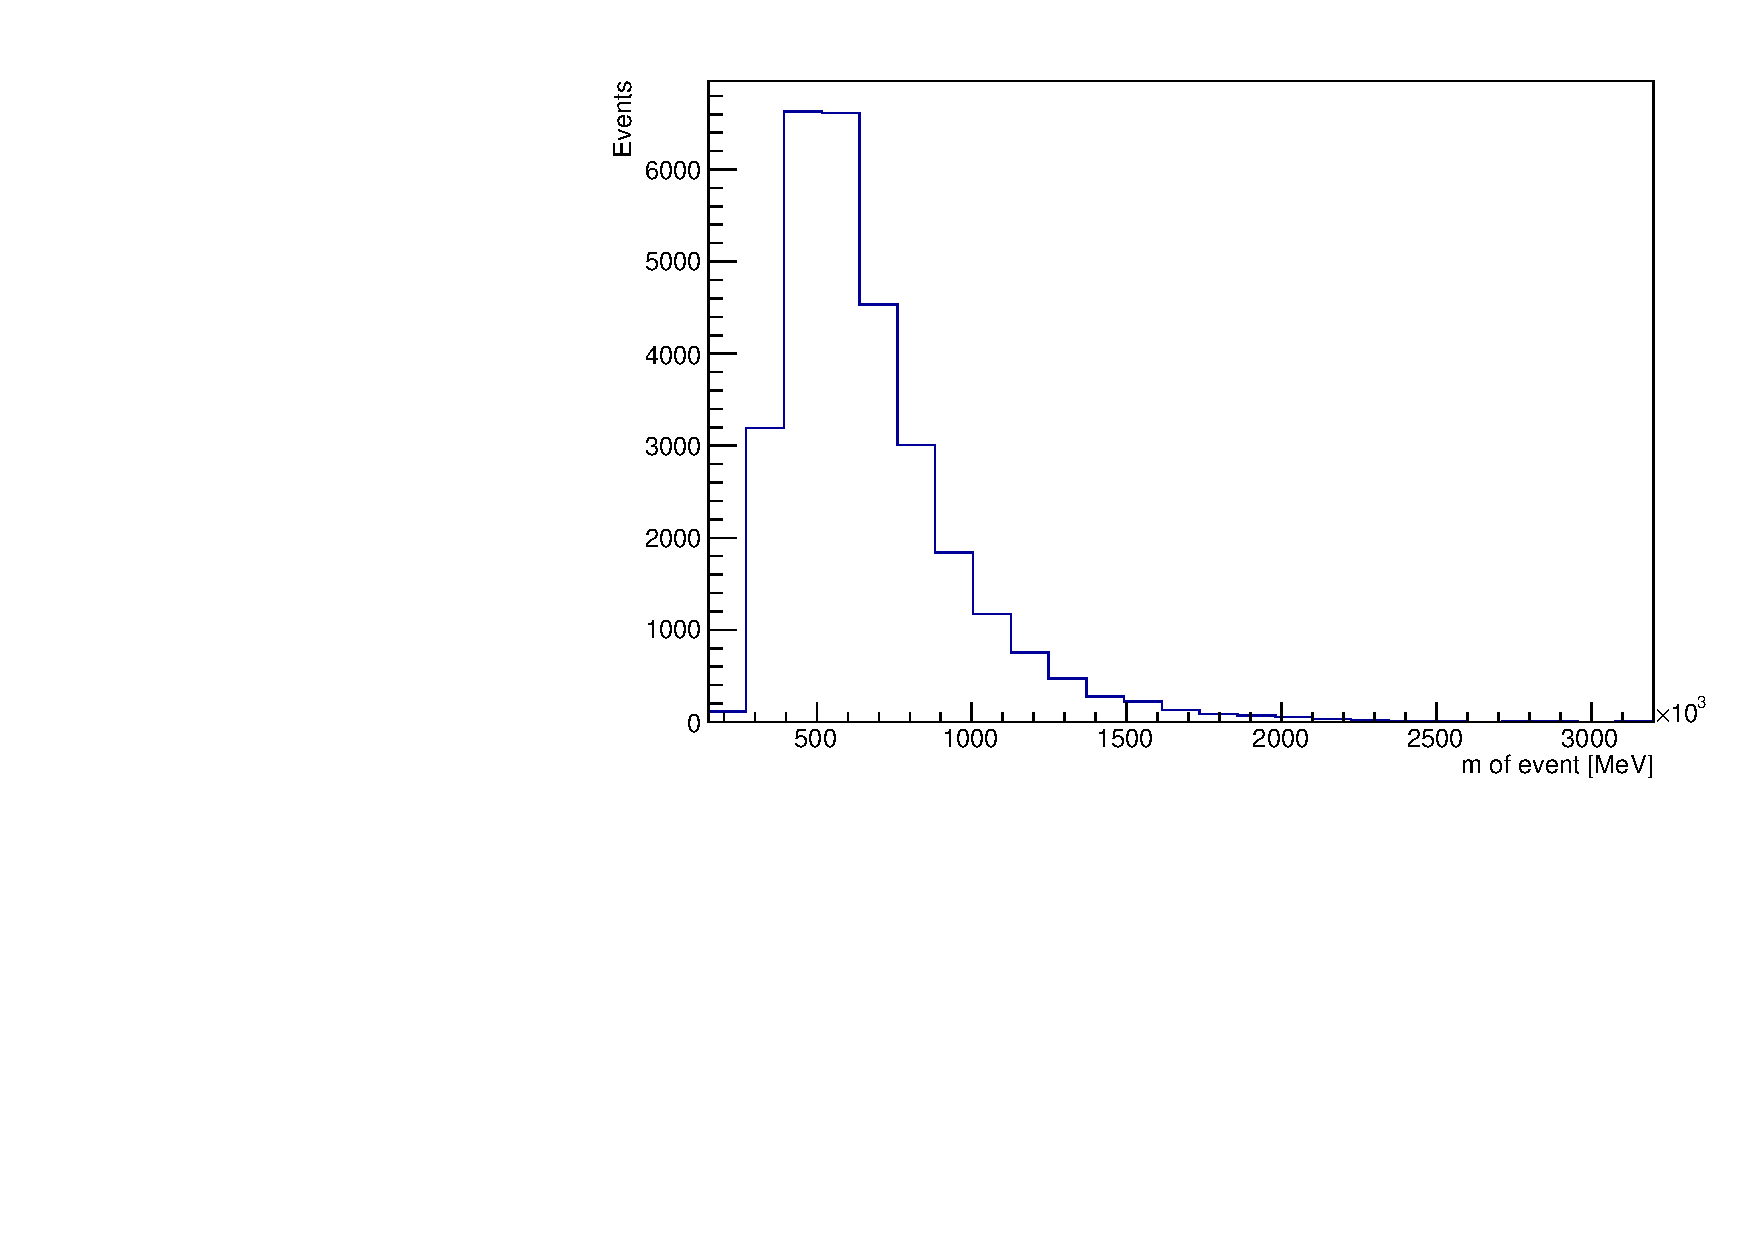
\includegraphics[width=\textwidth]{plots/discriminant/ttbar.el_dis4.pdf}%
    \caption{dis. 4, $t \overline{t}$}%
    \label{fig:5h}%
  \end{subfigure}%
  \caption{Histograms of the first four disciminants investigated for simulated $Z^\prime(1000 \, \si{\giga\eV})$- and $t \overline{t}$-events.}%
  \label{fig:5}%
\end{figure}

\begin{figure}[H]
  \begin{subfigure}{0.45\textwidth}%
    \centering%
    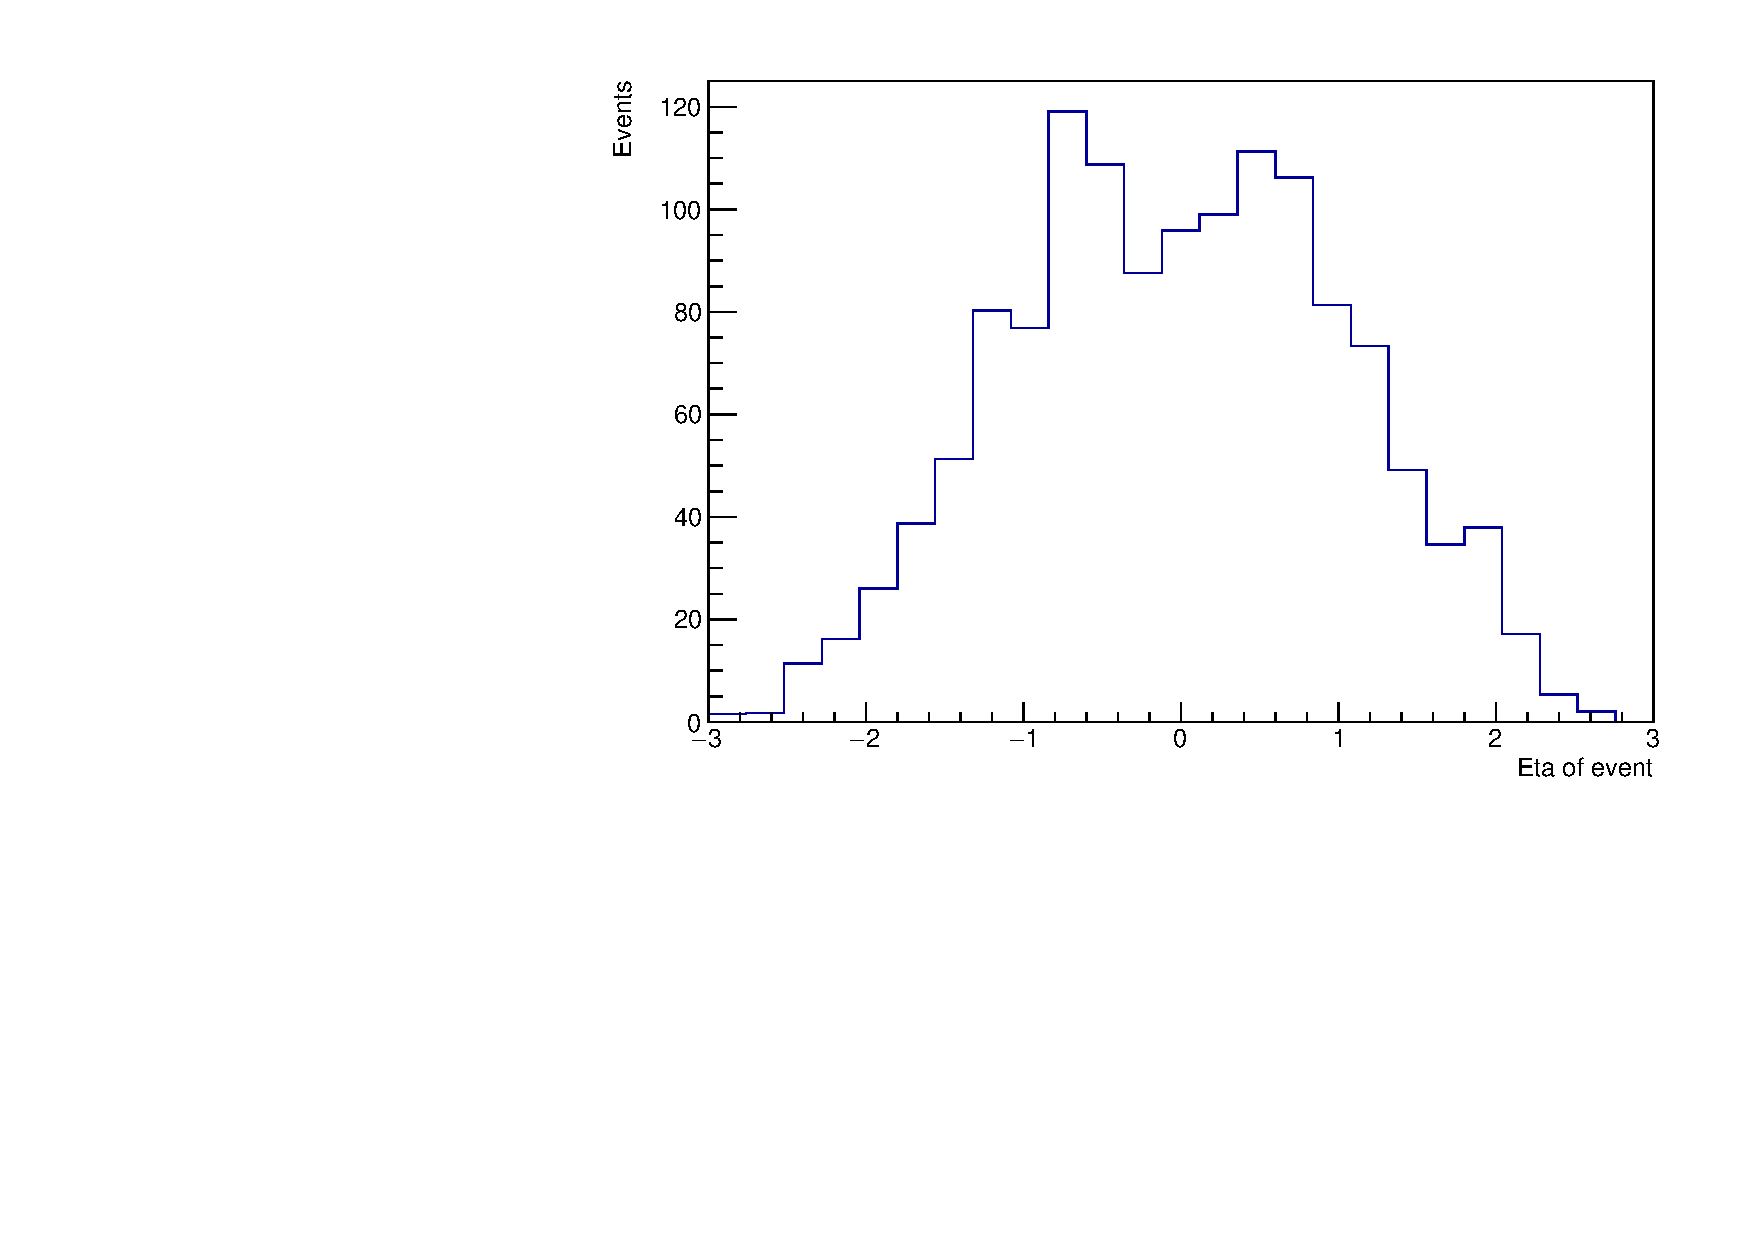
\includegraphics[width=\textwidth]{plots/discriminant/zprime1000.el_dis5.pdf}%
    \caption{dis. 5, $Z^\prime(1000 \, \si{\giga\eV})$}%
    \label{fig:6a}%
  \end{subfigure}%
  \hfill
  \begin{subfigure}{0.45\textwidth}%
    \centering%
    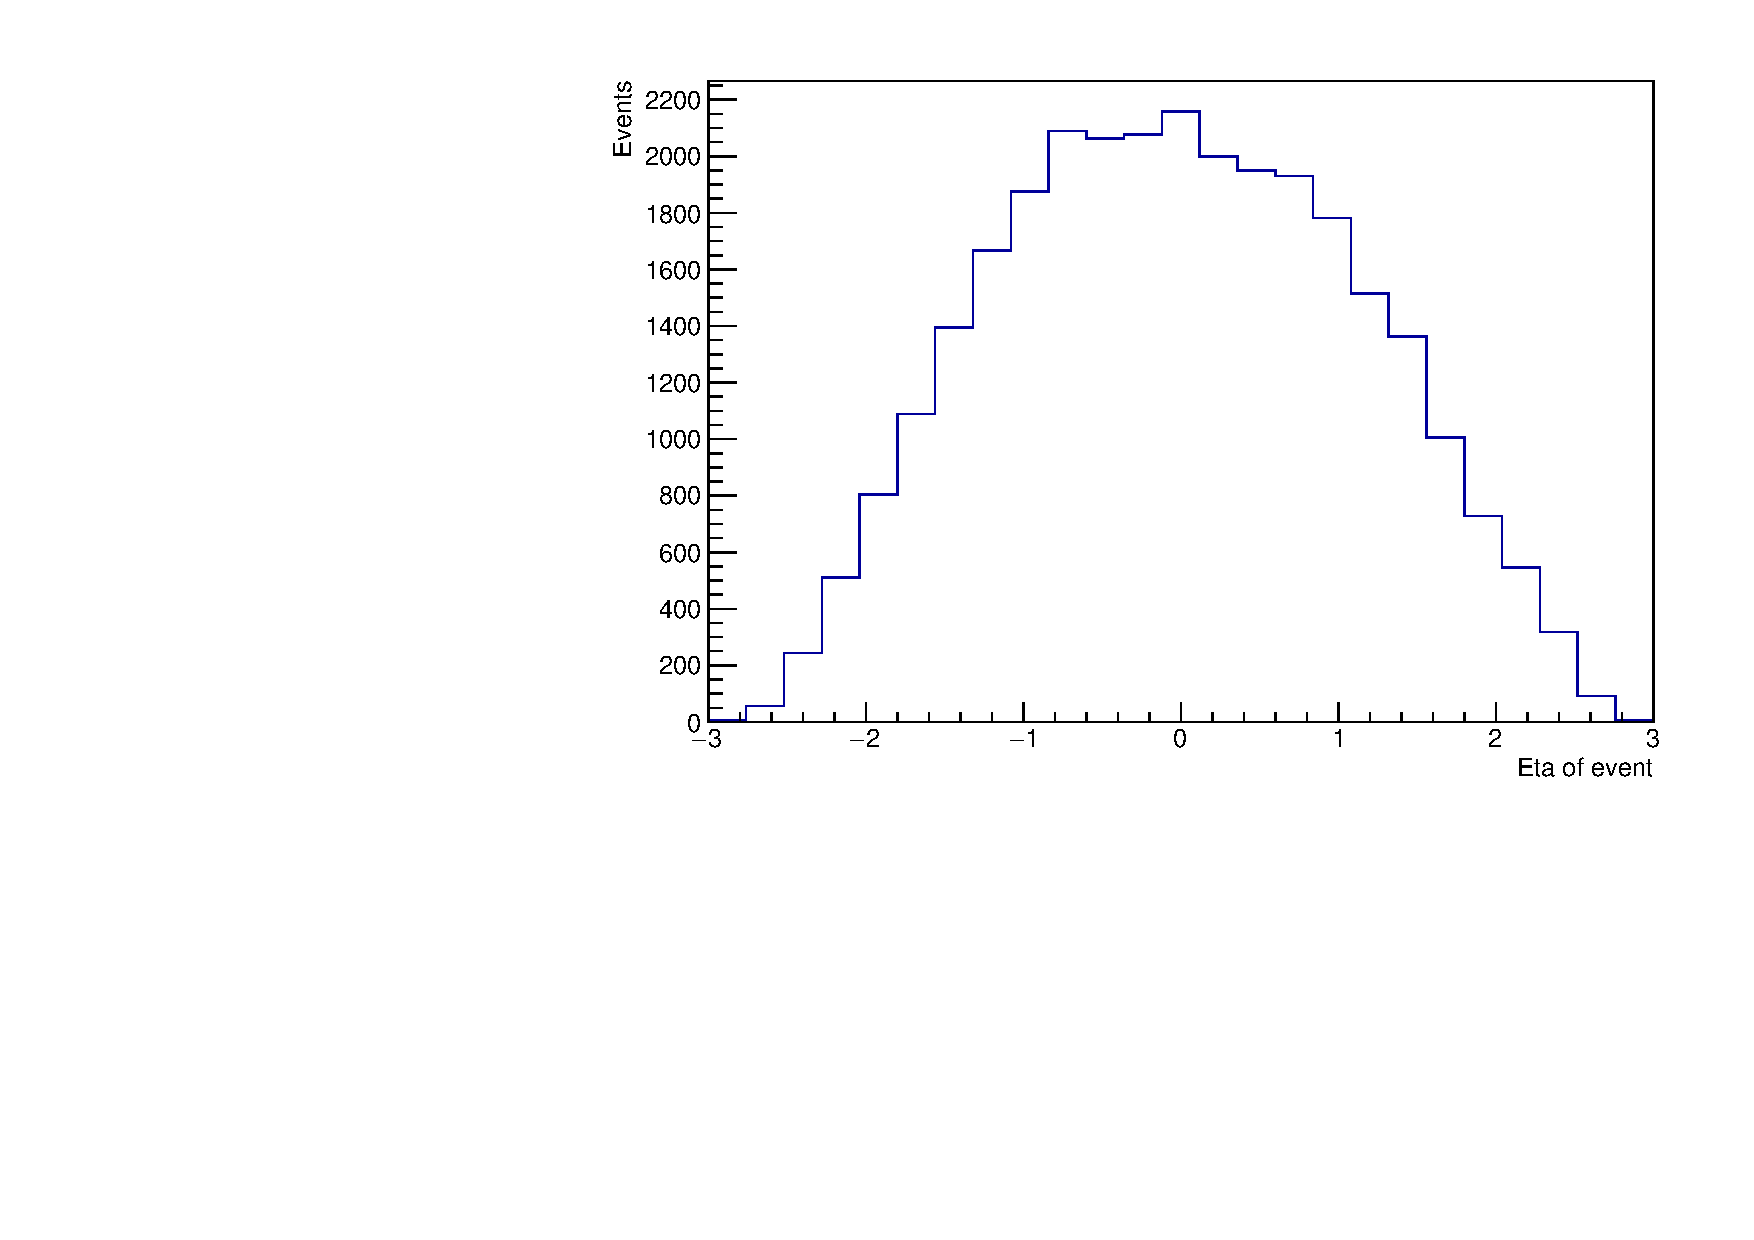
\includegraphics[width=\textwidth]{plots/discriminant/ttbar.el_dis5.pdf}%
    \caption{dis. 5, $t \overline{t}$}%
    \label{fig:6b}%
  \end{subfigure}%
  \caption{Histograms of the fifth disciminant investigated for simulated $Z^\prime(1000 \, \si{\giga\eV})$- and $t \overline{t}$-events.}%
  \label{fig:6}%
\end{figure}


\subsection{Agreement of simulation and data}
To test the agreement of the simulated samples and the data samples the number of expected evente $N = \mathcal{L} \sigma (A \cdot \epsilon)$ is calculated 
where $\mathcal{L} = 1000 \, \si{\femto\barn\tothe{-1}}$ is the integrated luminosity of the data sample used, \sigma is the cross section of the considered 
process listed in table \ref{tab:agree} and $(A \cdot \epsilon)$ is the efficiency of the selection listed in table \ref{tab:eff_b}.
The considered datasample contains $1112$ events after the selection while the number of expected events of the background processes is $716$. 
The number of expected events, where the determined values by process are shown in table \ref{tab:agree}, is clearly lower than the number of observed events. 
To further investigate discrepencies between the data samples and simulated samples the distributions of the quantities from section \ref{sec:sekunde} and the 
chosen final discriminant are created for the data sample and the simulated processes and shown in figure \ref{fig:6} and figure \ref{fig:7}.
All the distributions in figure \ref{fig:6} show very similar shapes for the data sample and simulated samples, but the excess of events in the 
data sample already observed in the number of total events is also visible. The same is true for the final discriminant. 
Since the oserved excess in the final discriminant is not concentrated is a peak as it would be expected for the products from the 
decay of a hypothetical particles this excess is not initially interpreted as a signal from a new particle. 

% sum expected events 715.5691039359999

\begin{table}[H]
  \centering
  \begin{tabular}{l|llll}
      sample           &  $N_\text{MC}$  & $\sigma$ / pb & w / $10^{-2}$& $N_\text{expected}$ \\
      \hline
      ttbar      & 7847944    & 252.82    &    3.22148068   &     4.11356659e+02       \\
      singletop  & 1468942    & 52.47     &    3.57195859   &     1.49062217e+01       \\
      diboson.el & 922521     & 29.41     &    3.18800331   &     1.09585726e-01       \\
      zjets      & 37422926   & 2516.2    &    6.72368590   &     8.88950051e+00       \\
      wjets      & 66536222   & 36214     &   54.42749660   &     2.80307137e+02       \\
      zprime400  & 100000     & 110       &  110.00000000   &     2.73528970e+03       \\
      zprime500  & 100000     & 82        &   82.00000000   &     3.37859483e+03       \\
      zprime750  & 100000     & 20        &   20.00000000   &     4.85756000e+02       \\
      zprime1000 & 100000     & 5.5       &    5.50000000   &     5.36619875e+01       \\
      zprime1250 & 100000     & 1.9       &    1.90000000   &     6.78607800e+00       \\
      zprime1500 & 100000     & 0.83e     &    0.83000000   &     1.27974886e+00       \\
      zprime1750 & 100000     & 0.3       &    0.30000000   &     1.70668800e-01       \\
      zprime2000 & 100000     & 0.14      &    0.14000000   &     3.36669200e-02       \\
      zprime2250 & 100000     & 0.067     &    0.06700000   &     7.50381240e-03       \\
      zprime2500 & 100000     & 0.035     &    0.03500000   &     1.93160450e-03       \\
      zprime3000 & 100000     & 0.012     &    0.01200000   &     2.08807200e-04       \\
      \end{tabular}
\caption{The efficiency of the selection after the application of subsequent cuts (6-7).}
\label{tab:agree}

  \end{table}

\begin{figure}[H]%
  \begin{subfigure}{0.48\textwidth}%
    \centering%
    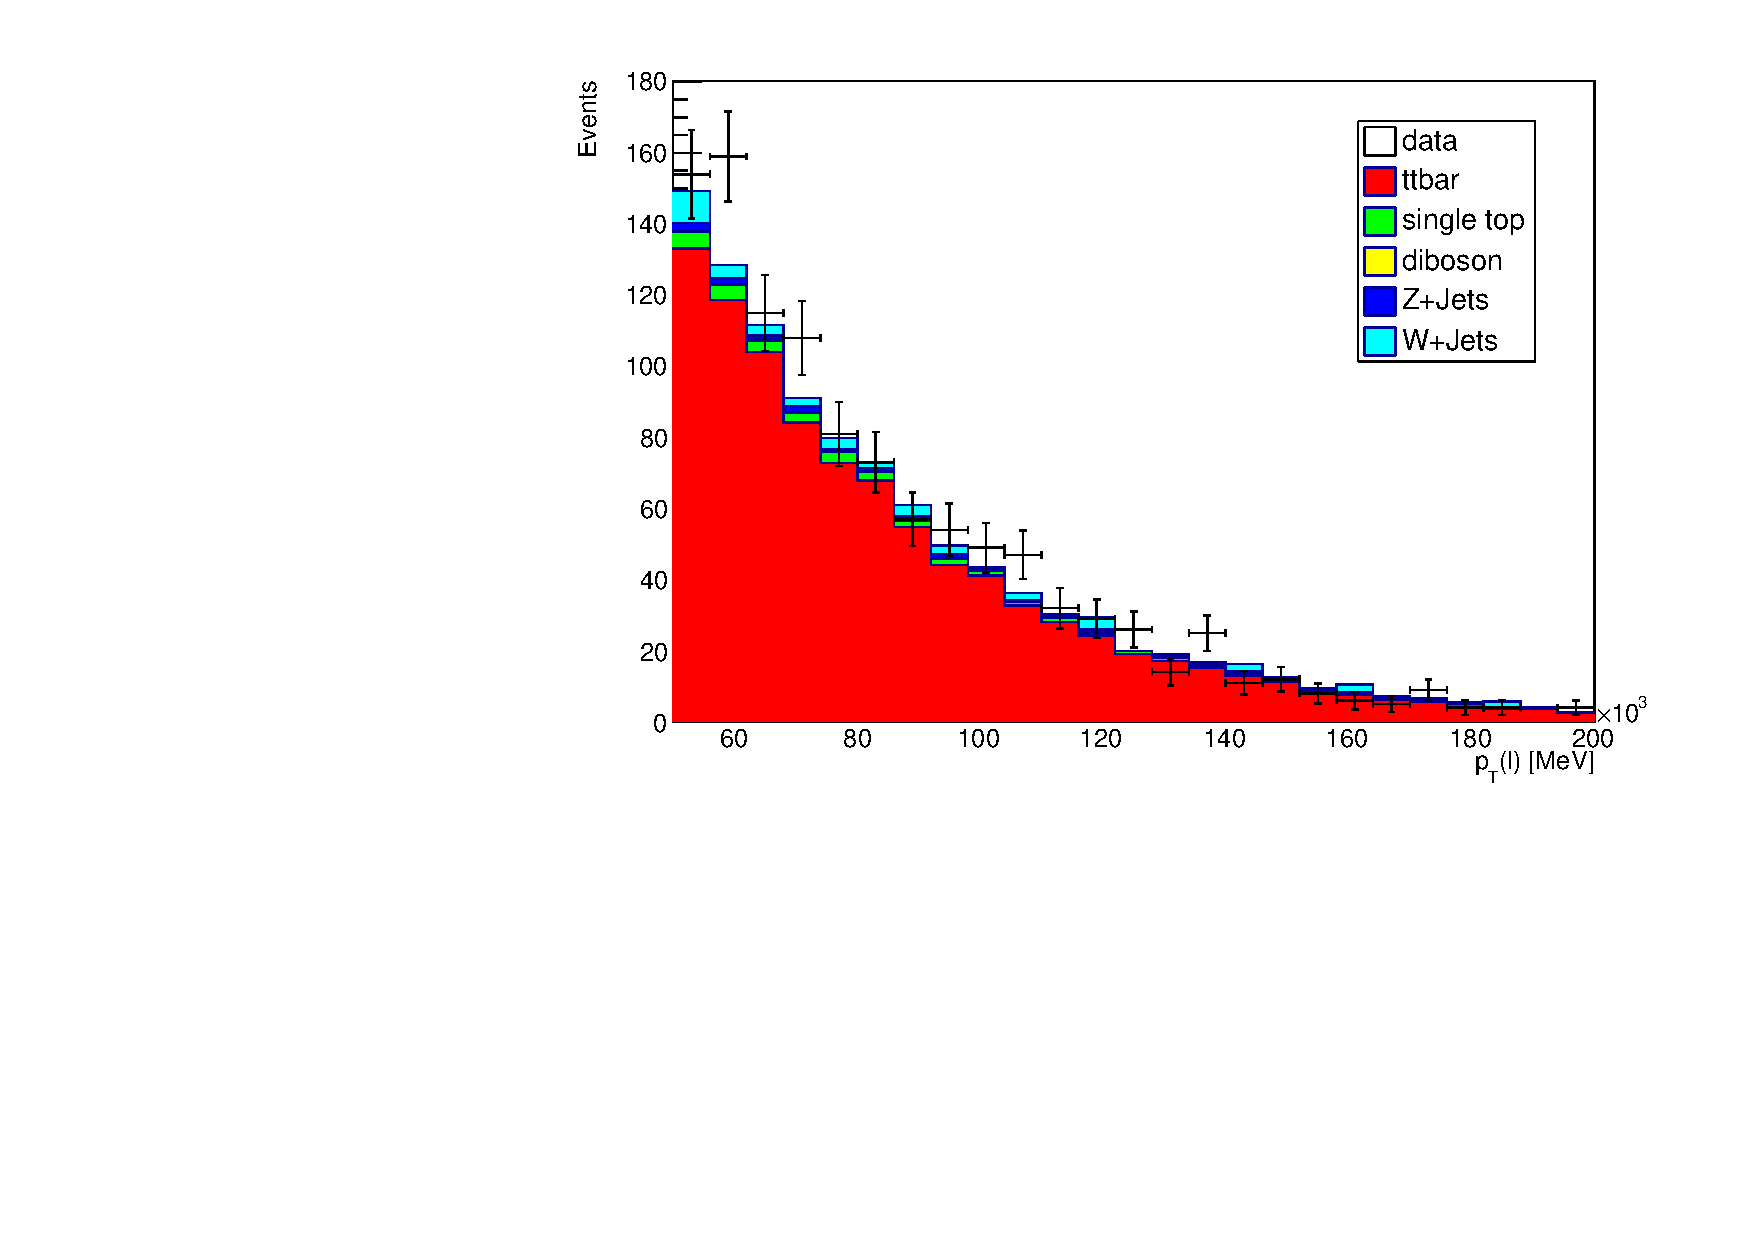
\includegraphics[width=\textwidth]{plots/comparism/lep_pt.pdf}%
    \caption{Transverse momentum of the lepton.}%
    \label{fig:6a}%
  \end{subfigure}%
  \hfill
  \begin{subfigure}{0.48\textwidth}%
    \centering%
    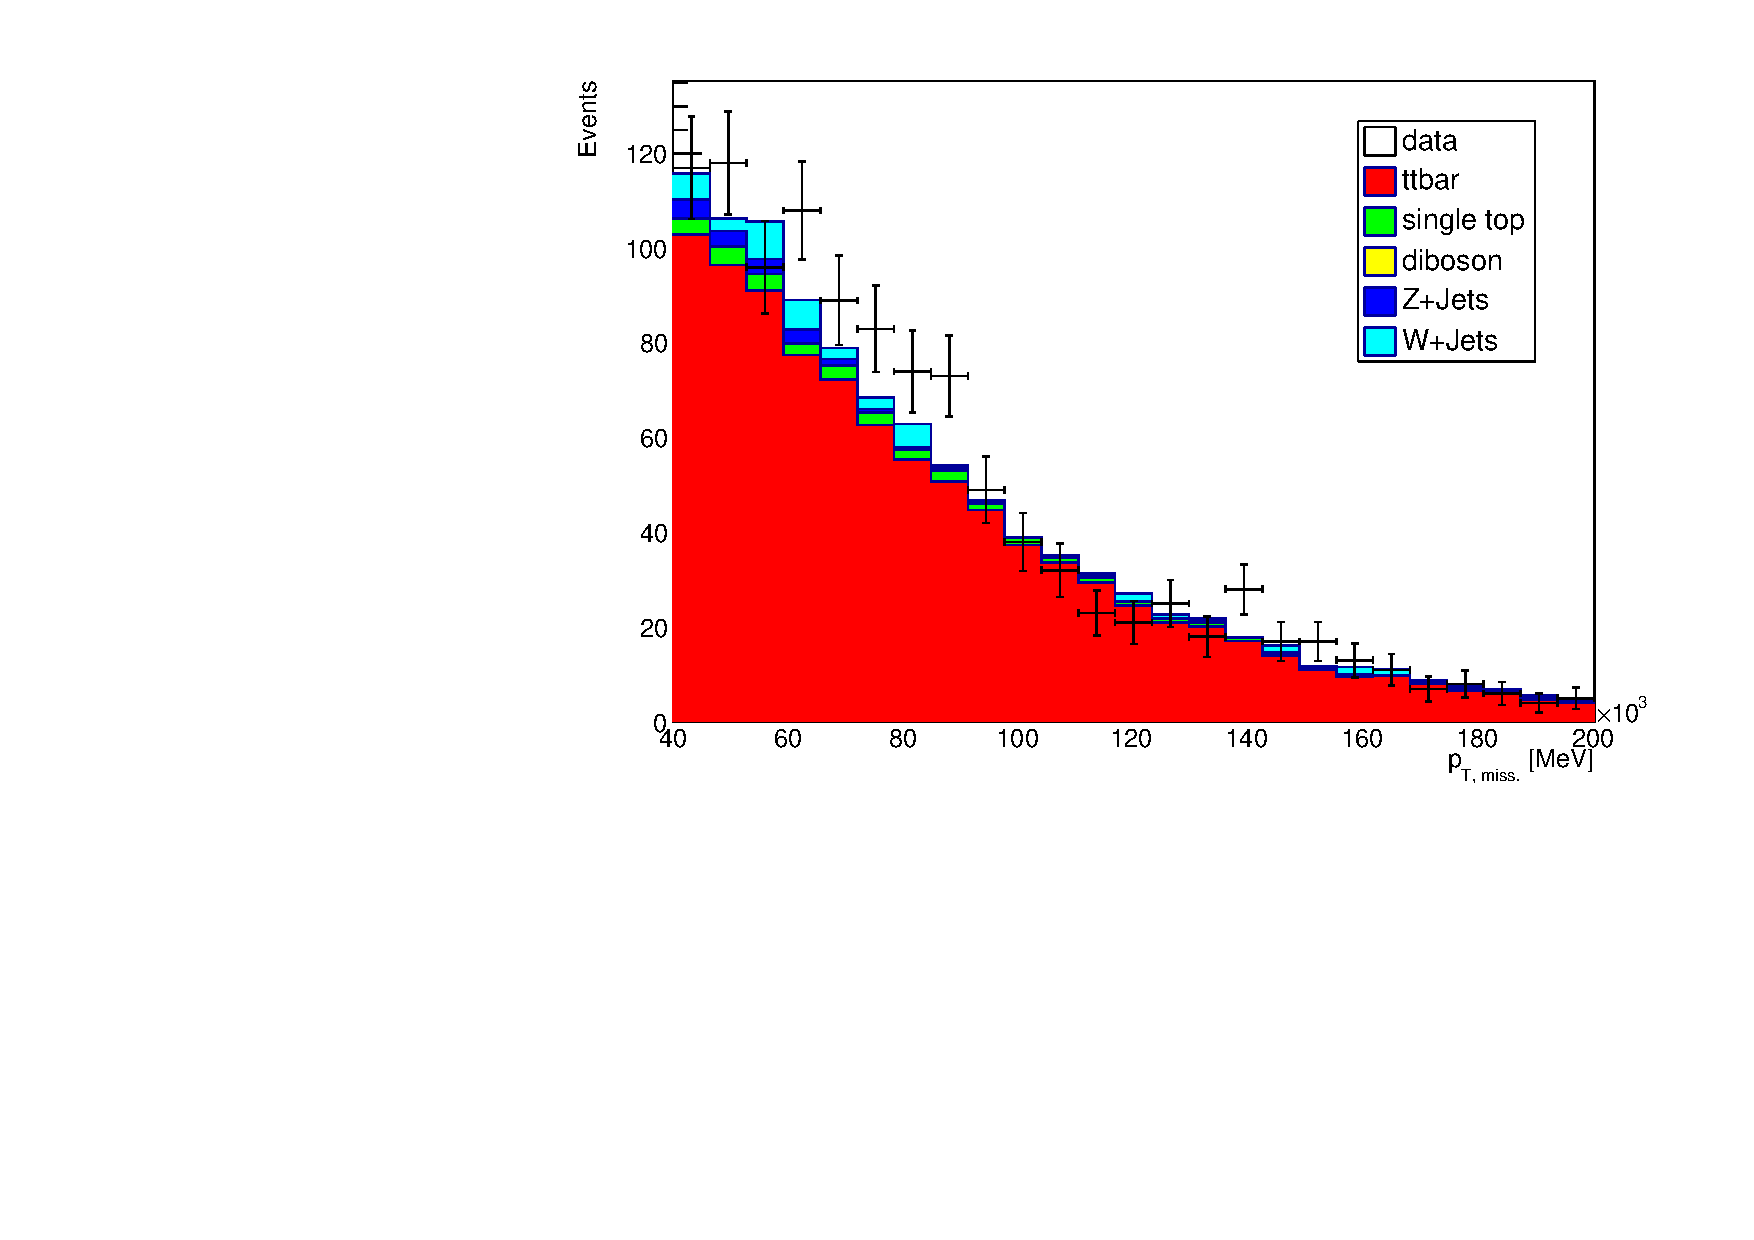
\includegraphics[width=\textwidth]{plots/comparism/met_et.pdf}%
    \caption{Missing transverse momentum of the lepton.}%
    \label{fig:6b}%
  \end{subfigure}%

  \begin{subfigure}{0.45\textwidth}%
    \centering%
    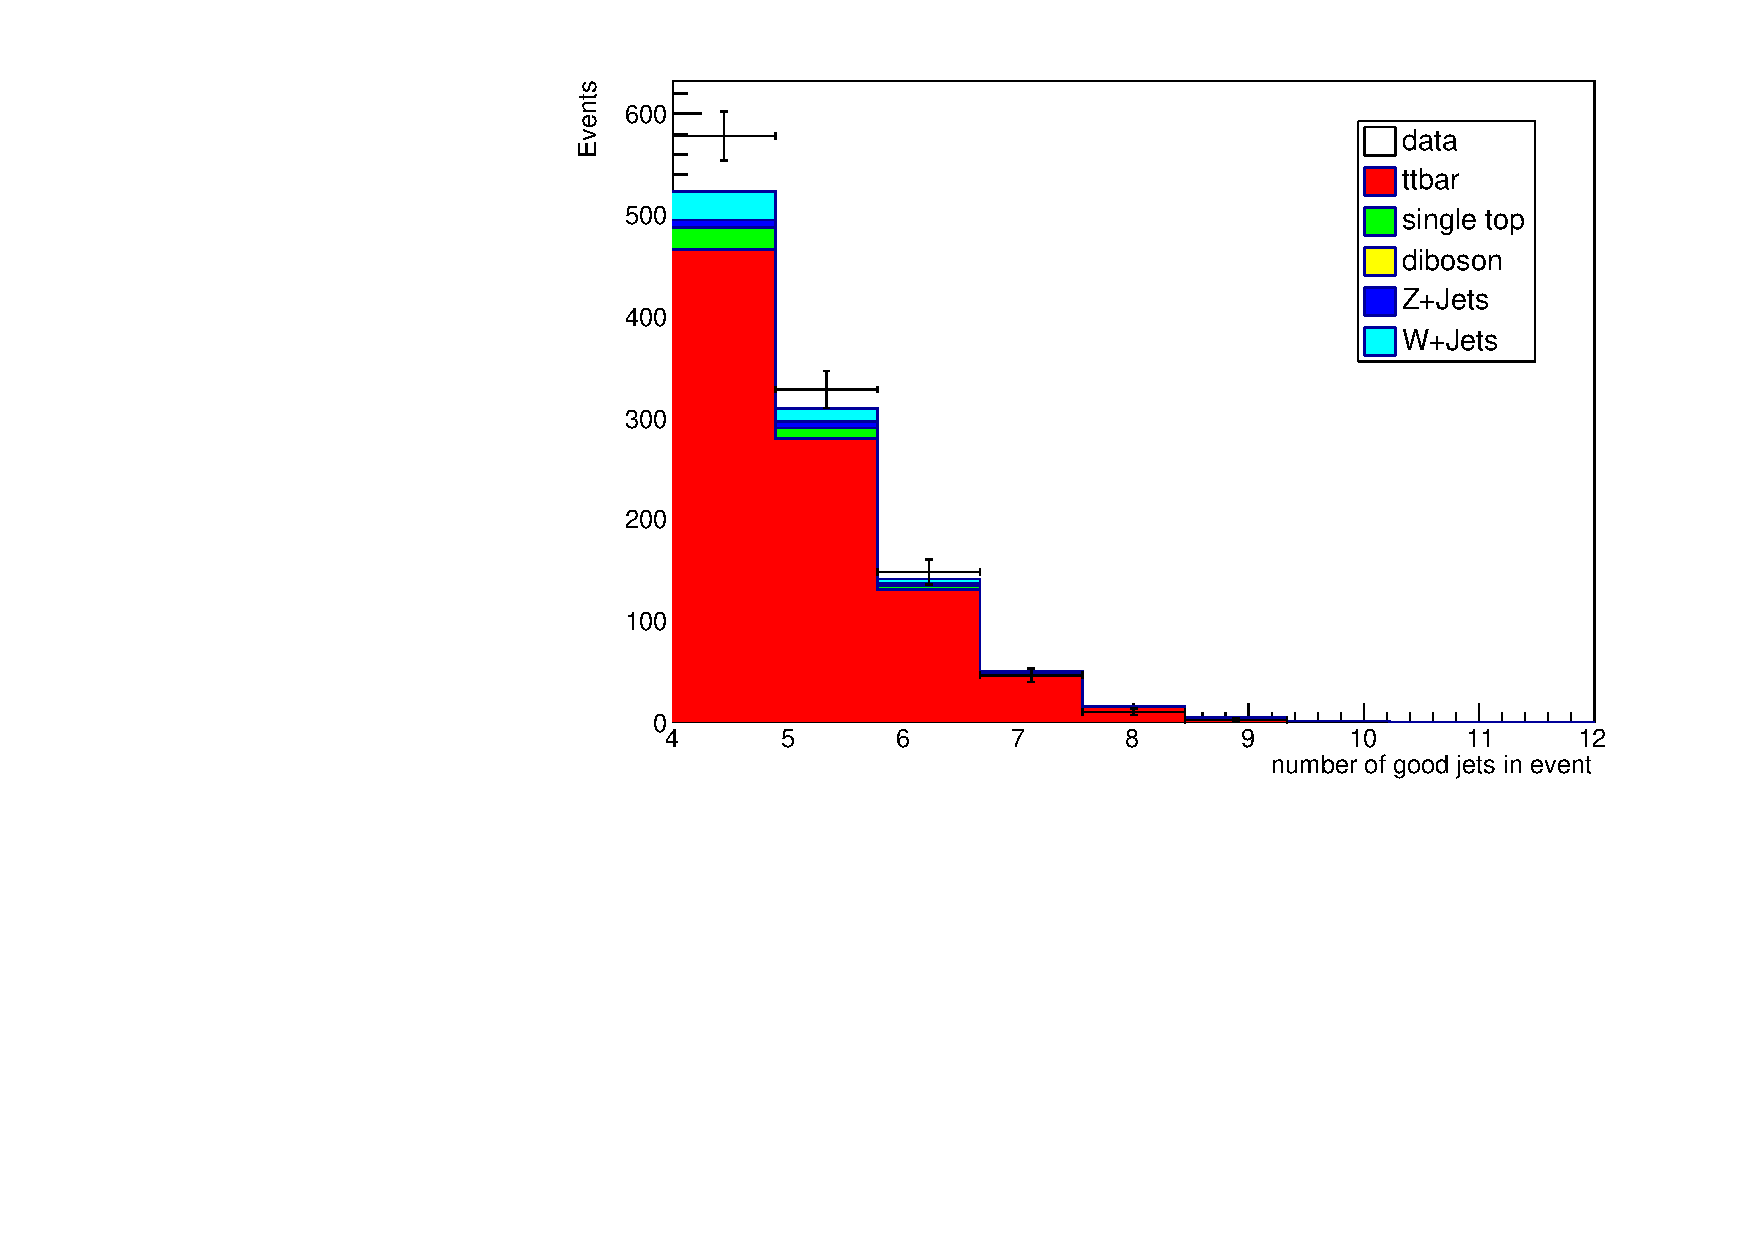
\includegraphics[width=\textwidth]{plots/comparism/jet_goot.pdf}%
    \caption{Number of good jets.}%
    \label{fig:6c}%
  \end{subfigure}%
  \hfill
  \begin{subfigure}{0.45\textwidth}%
    \centering%
    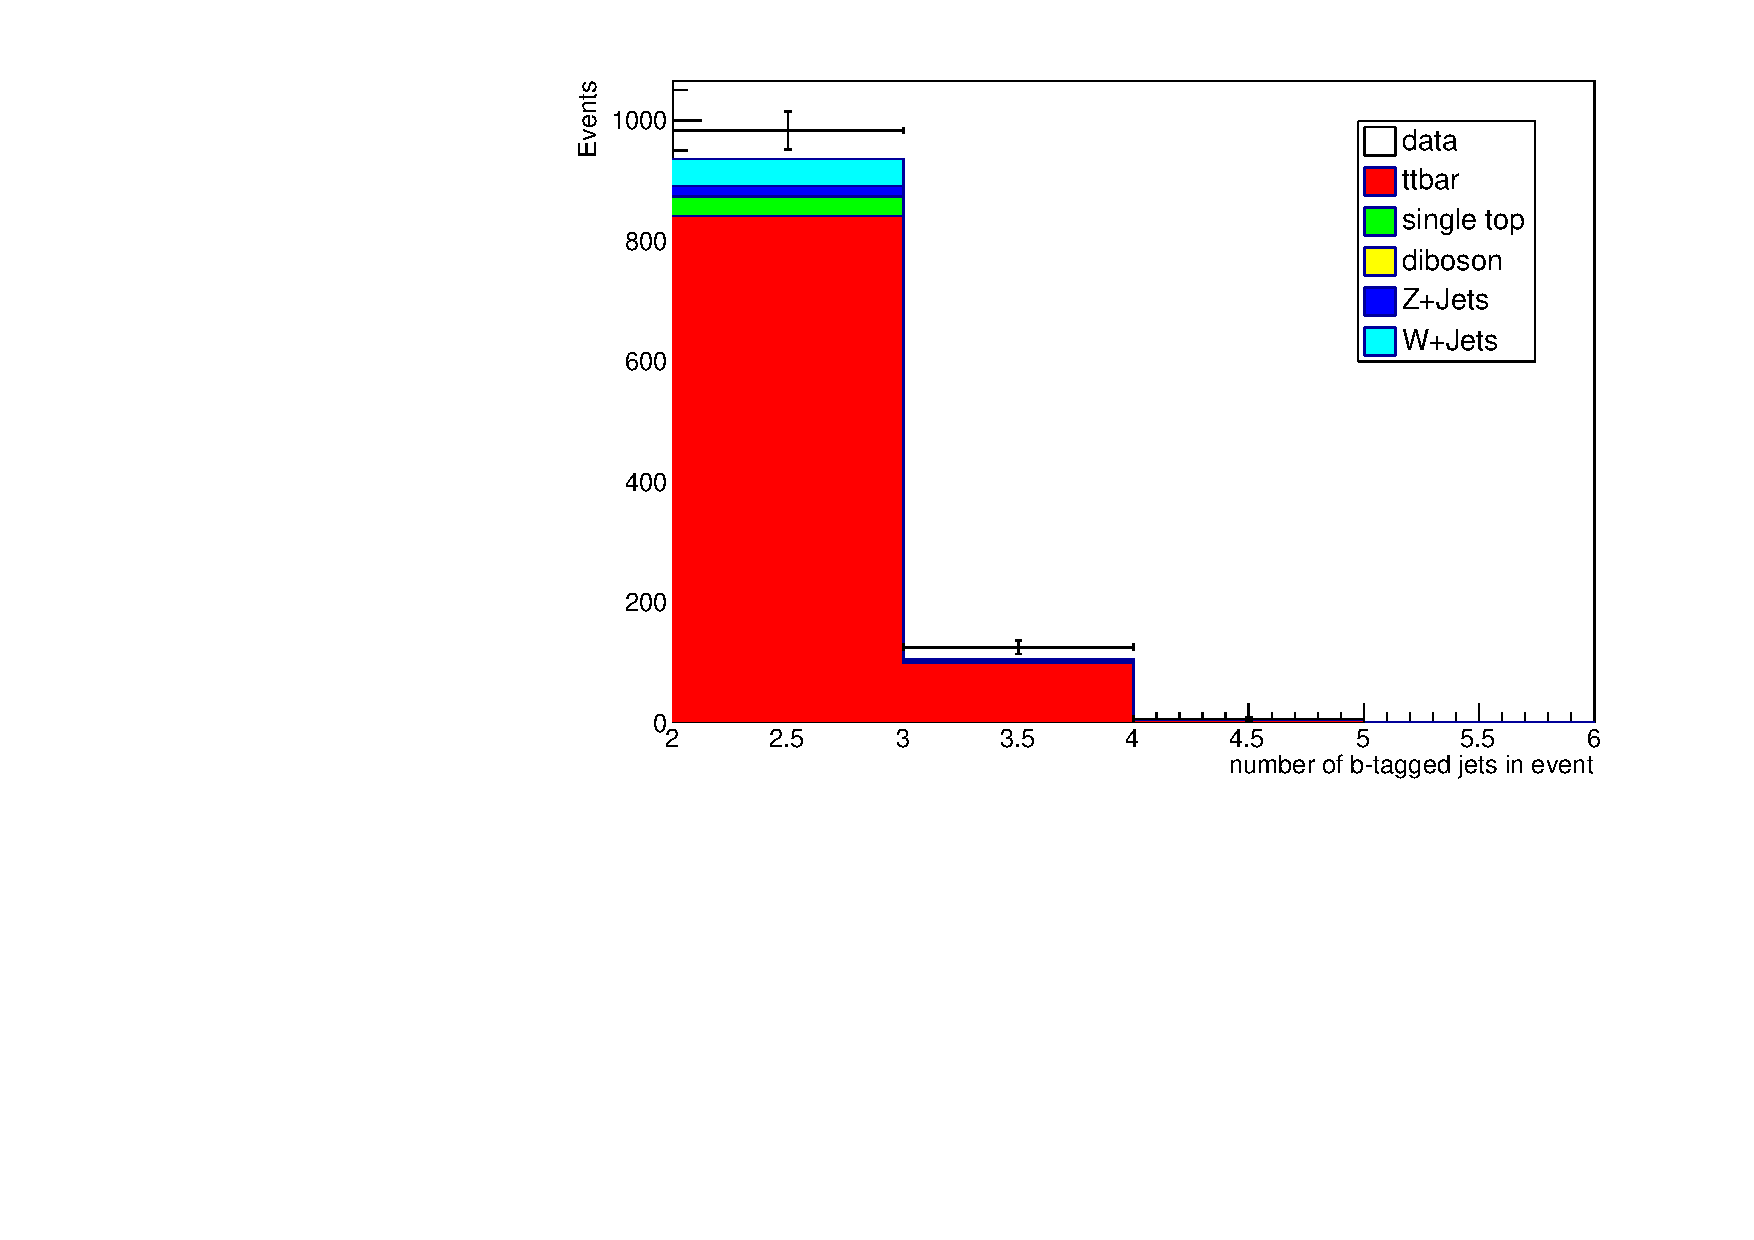
\includegraphics[width=\textwidth]{plots/comparism/jet_b_tagged.pdf}%
    \caption{Number of b-tagged jets.}%
    \label{fig:6d}%
  \end{subfigure}%

  \begin{subfigure}{0.45\textwidth}%
    \centering%
    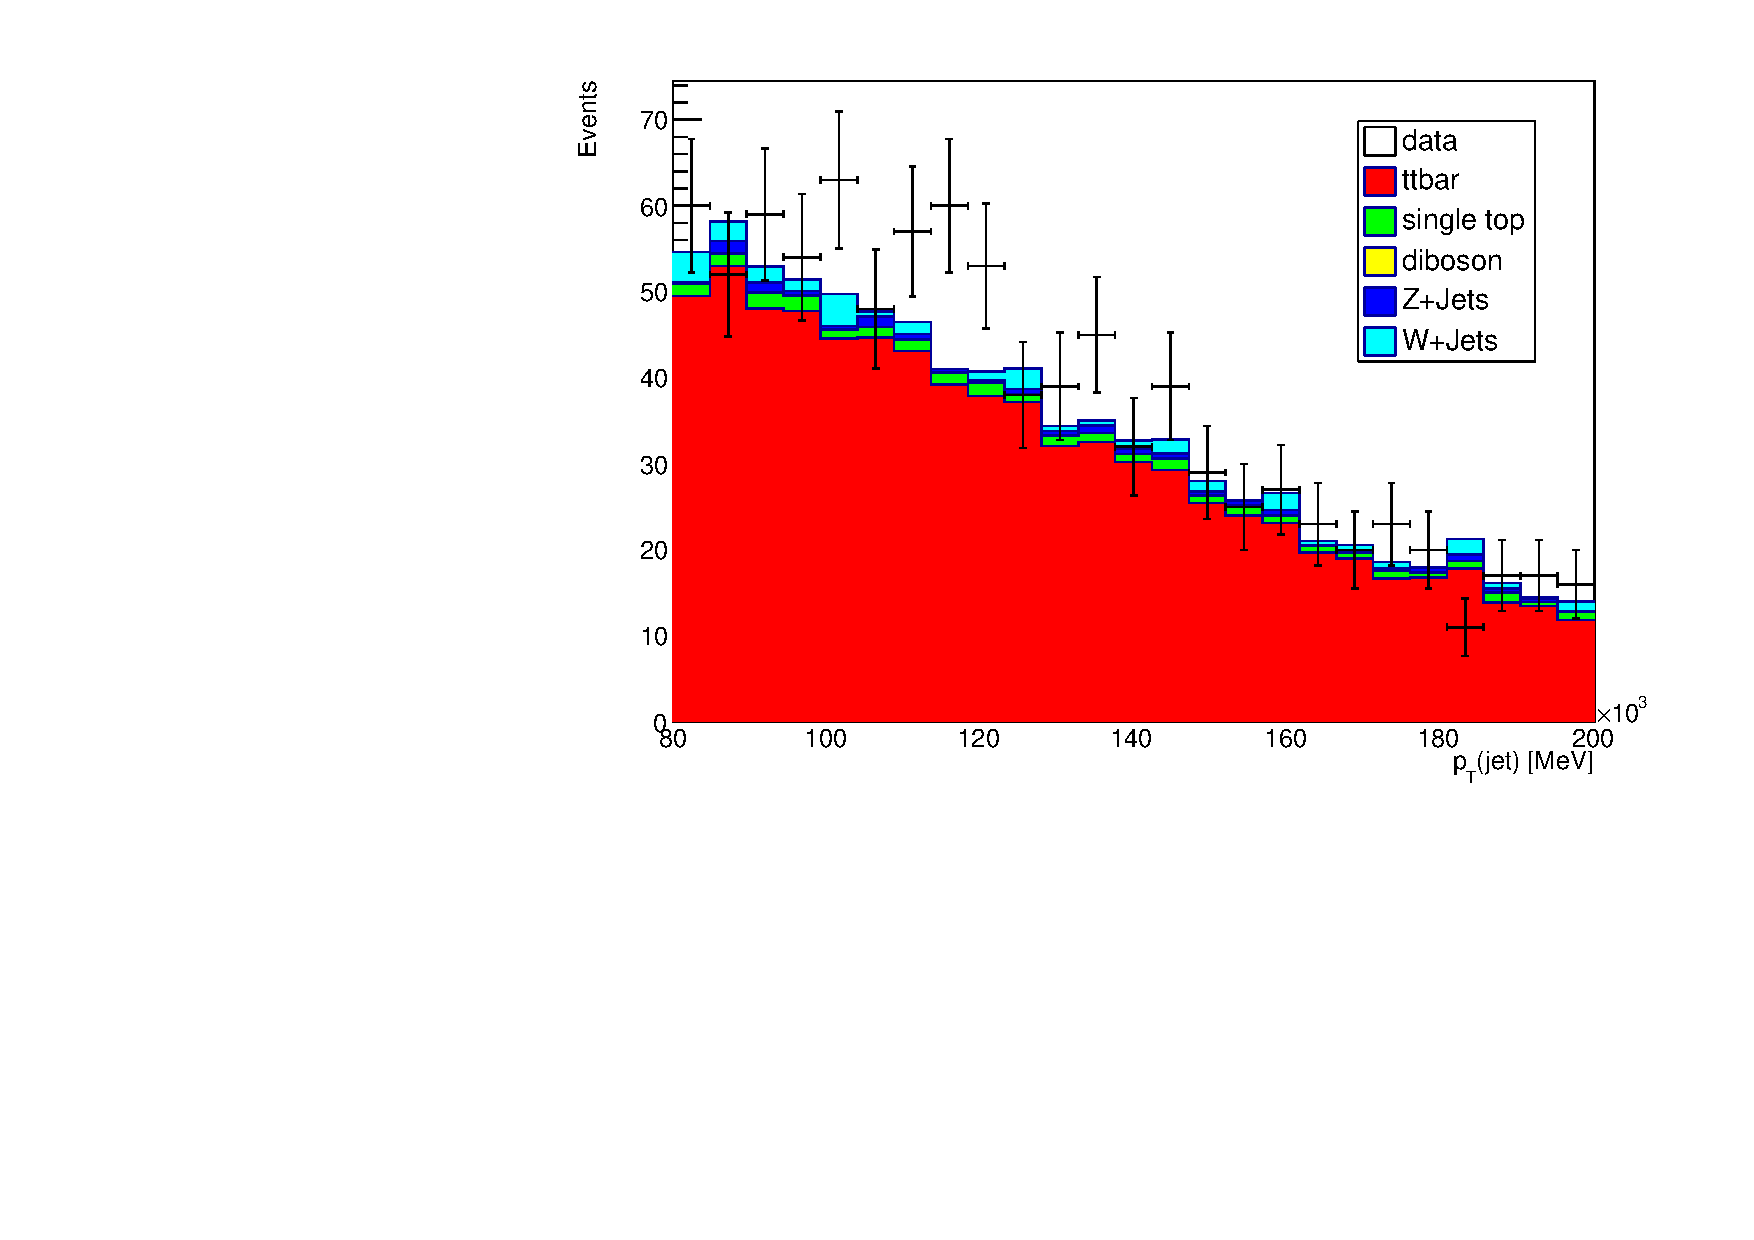
\includegraphics[width=\textwidth]{plots/comparism/jet_pt_max.pdf}%
    \caption{Transverse momentum of jet with maximal transverse momentum in each event.}%
    \label{fig:6e}%
  \end{subfigure}%
  \hfill
  \begin{subfigure}{0.45\textwidth}%
    \centering%
    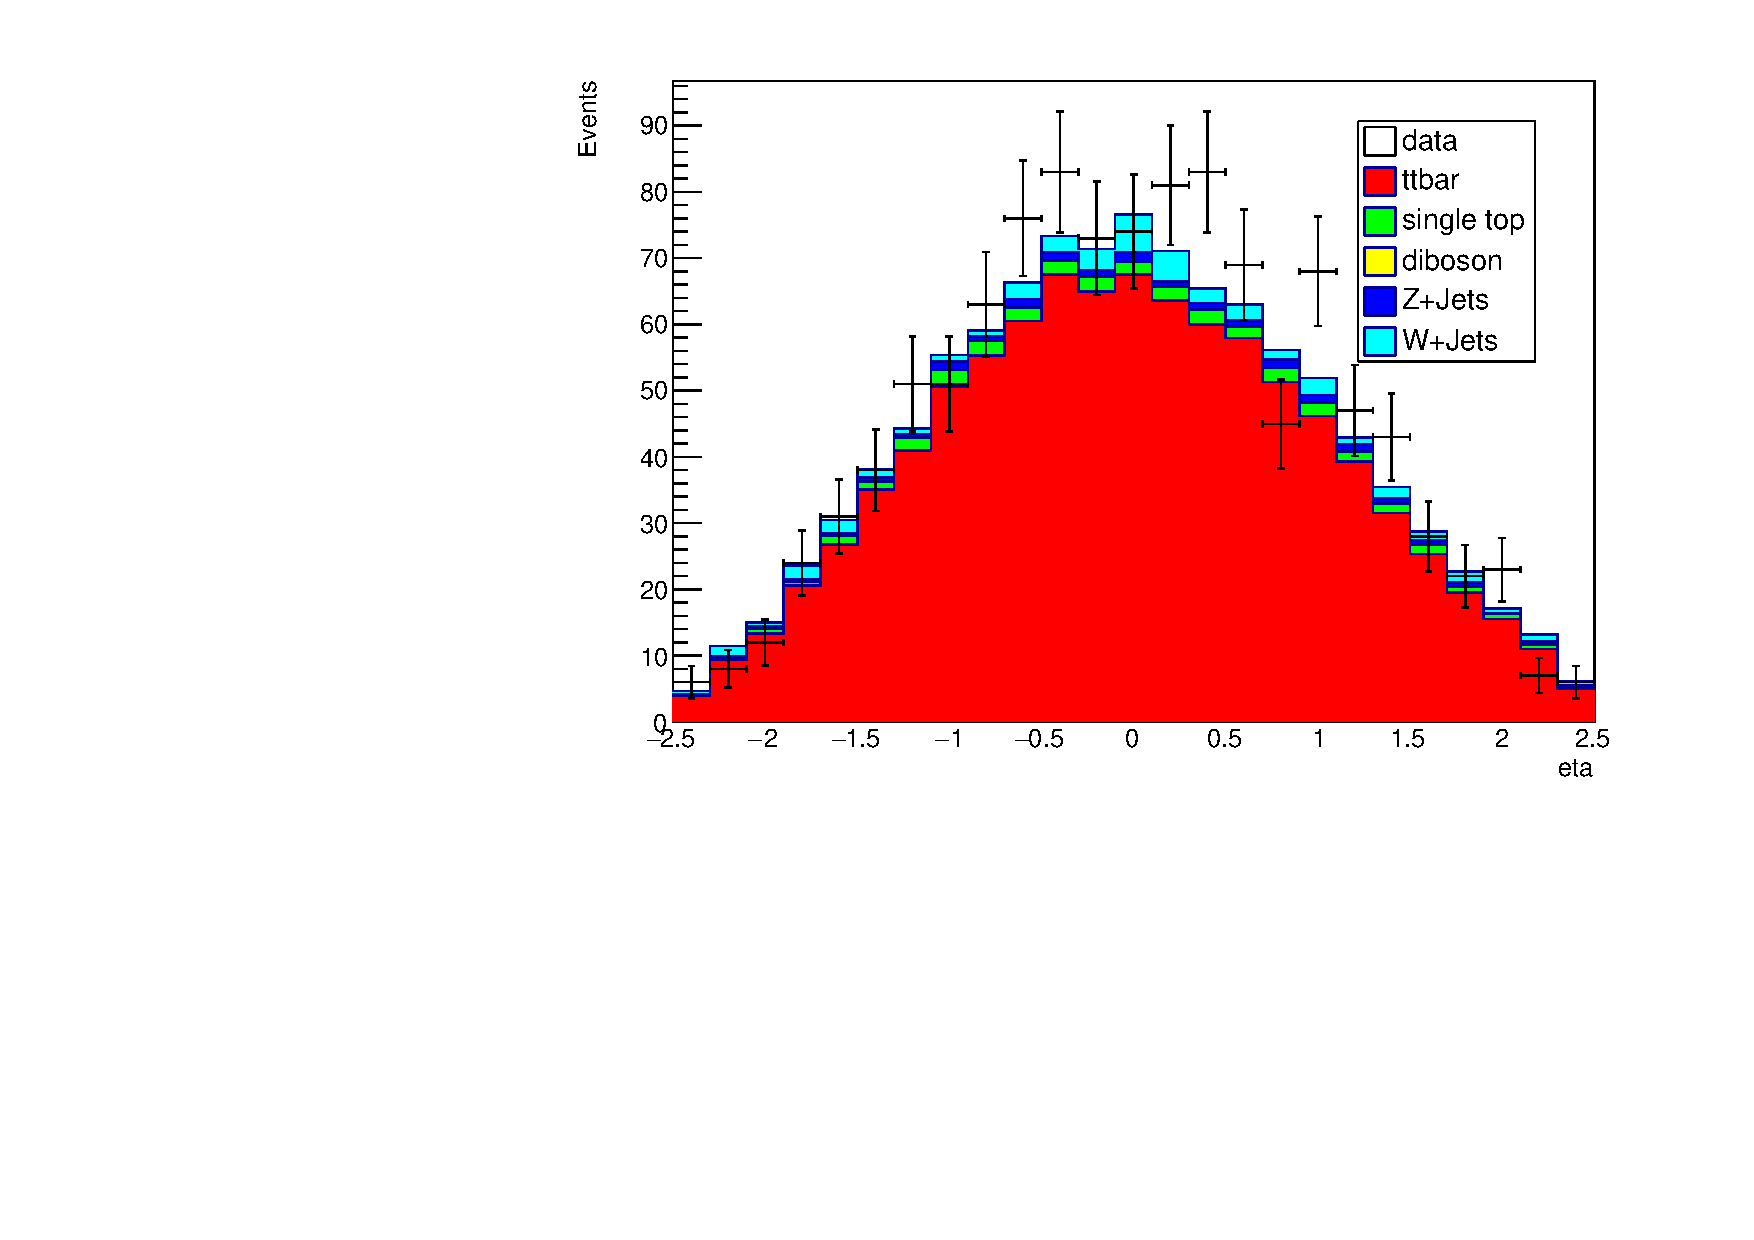
\includegraphics[width=\textwidth]{plots/comparism/jet_eta_max.pdf}%
    \caption{Pseudorapidity of jet with maximal transverse momentum in each event.}%
    \label{fig:6f}%
  \end{subfigure}%

  \begin{subfigure}{0.45\textwidth}%
    \centering%
    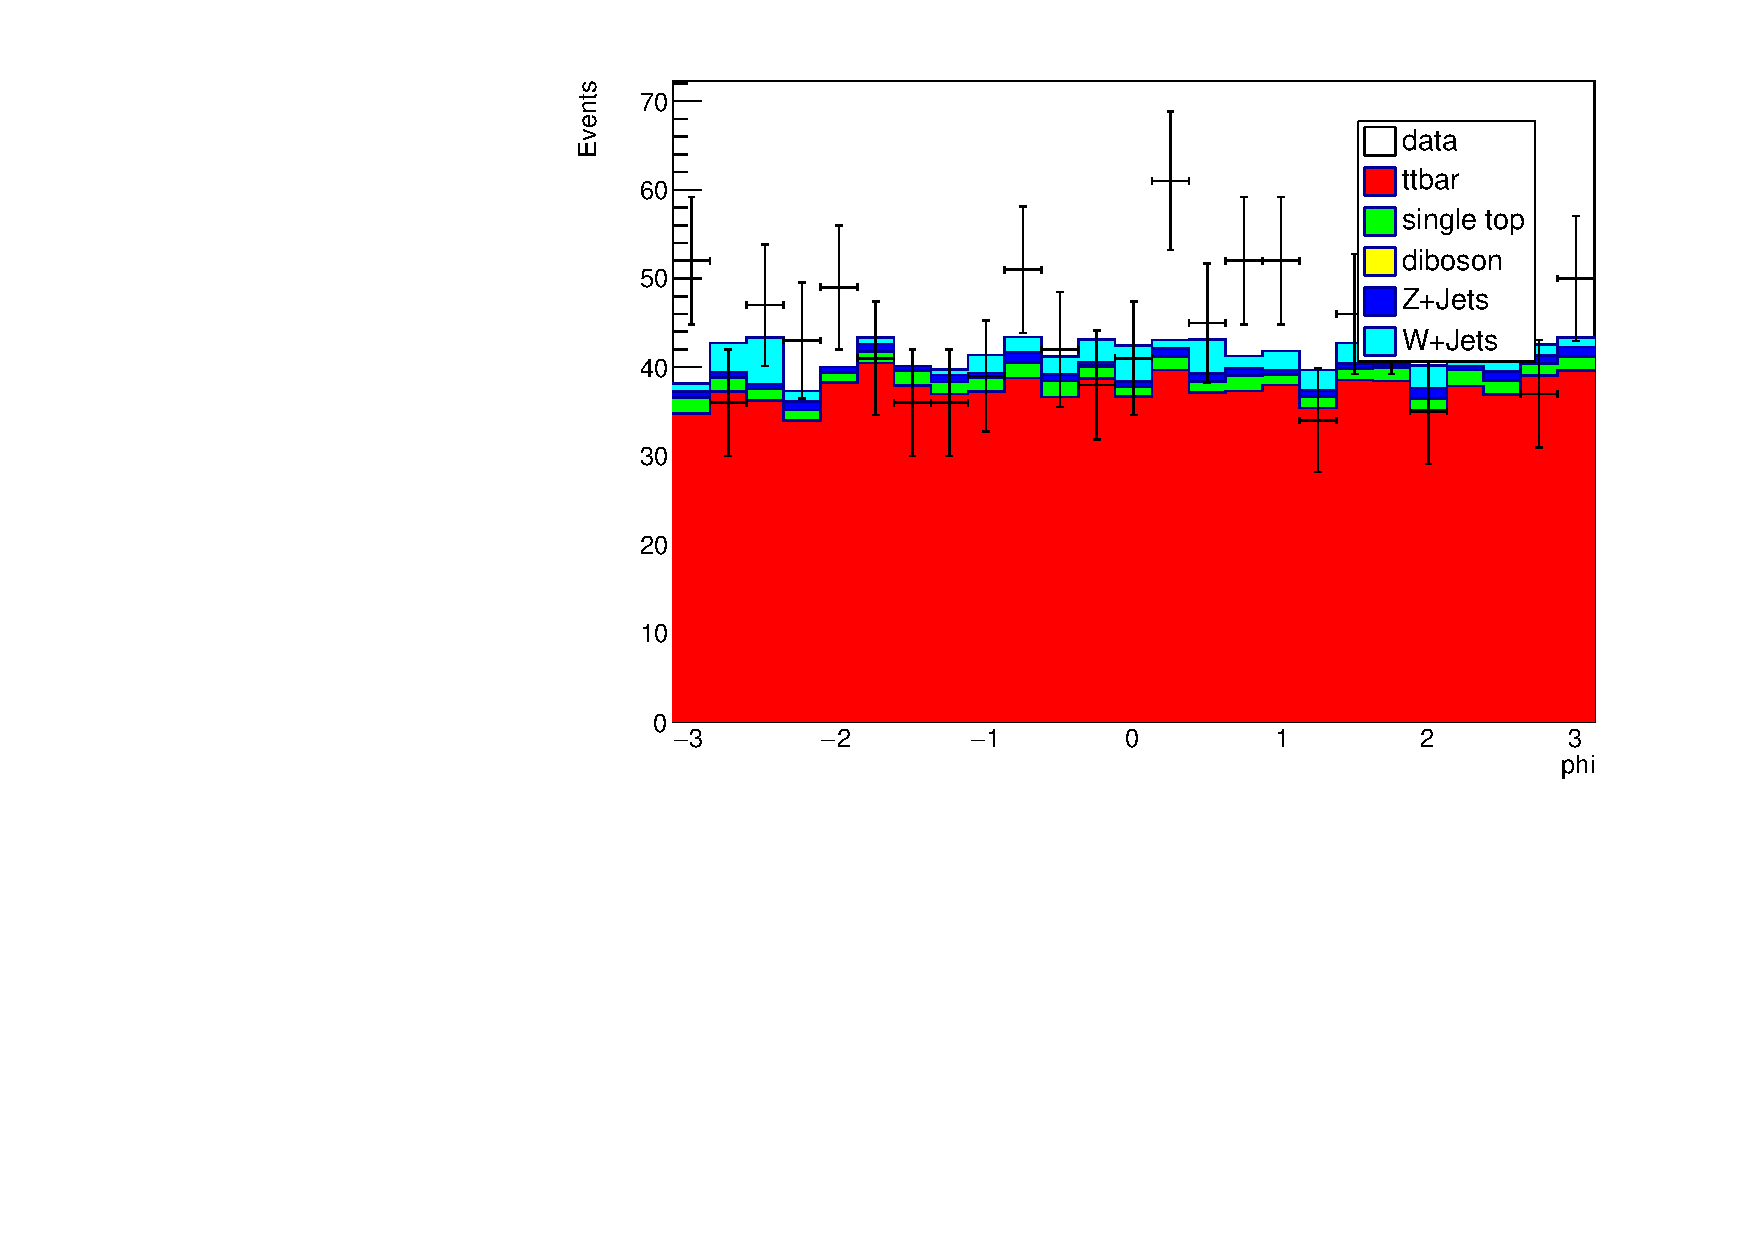
\includegraphics[width=\textwidth]{plots/comparism/jet_phi_max.pdf}%
    \caption{Azimuthal angle of jet with maximal transverse momentum in each event.}%
    \label{fig:6g}%
  \end{subfigure}%
  \hfill
  \begin{subfigure}{0.45\textwidth}%
    \centering%
    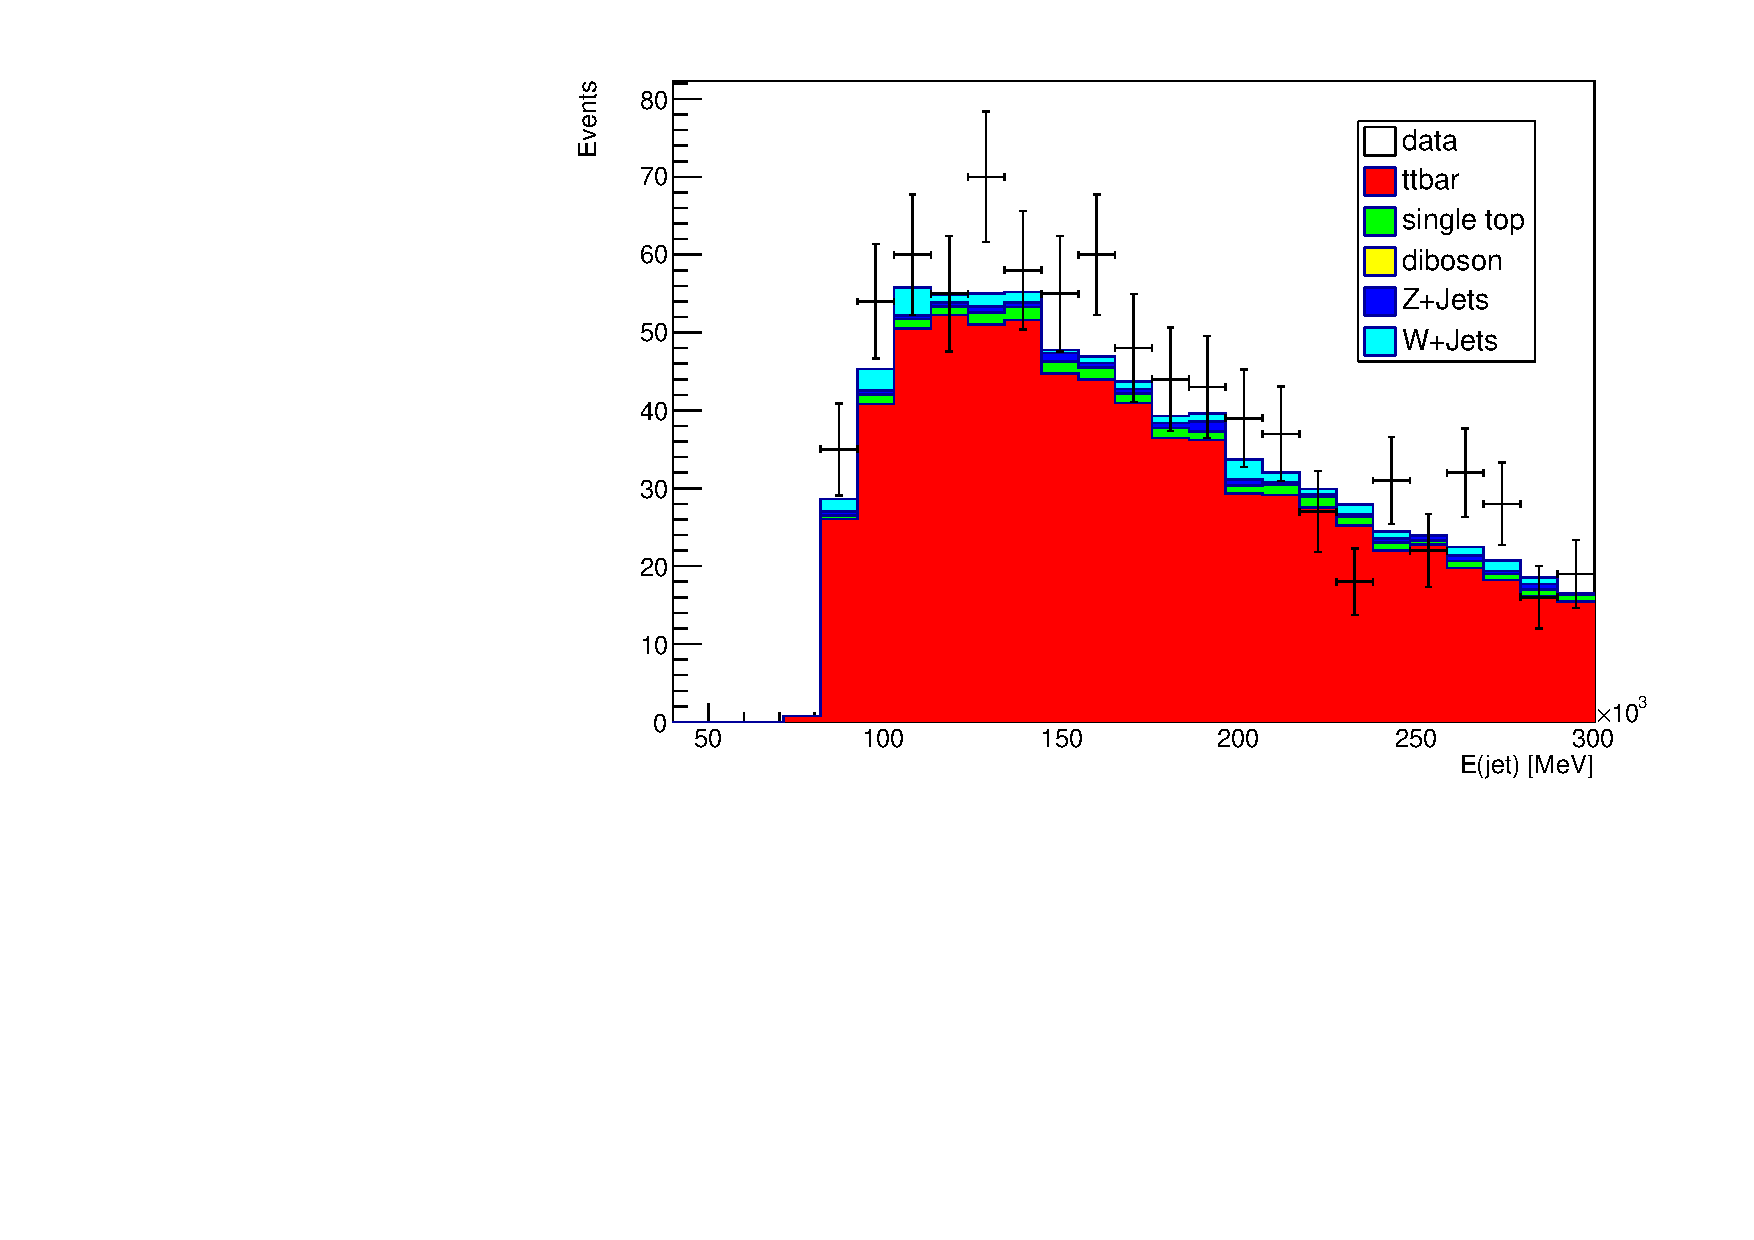
\includegraphics[width=\textwidth]{plots/comparism/jet_E_max.pdf}%
    \caption{Energy of jet with maximal transverse momentum in each event.}%
    \label{fig:6h}%
  \end{subfigure}%
  \caption{Stacked plots of the fundamental distributions investigated in section \ref{sec:sekunde}.}%
  \label{fig:6}%
\end{figure}

\begin{figure}[tb]
  \centering
  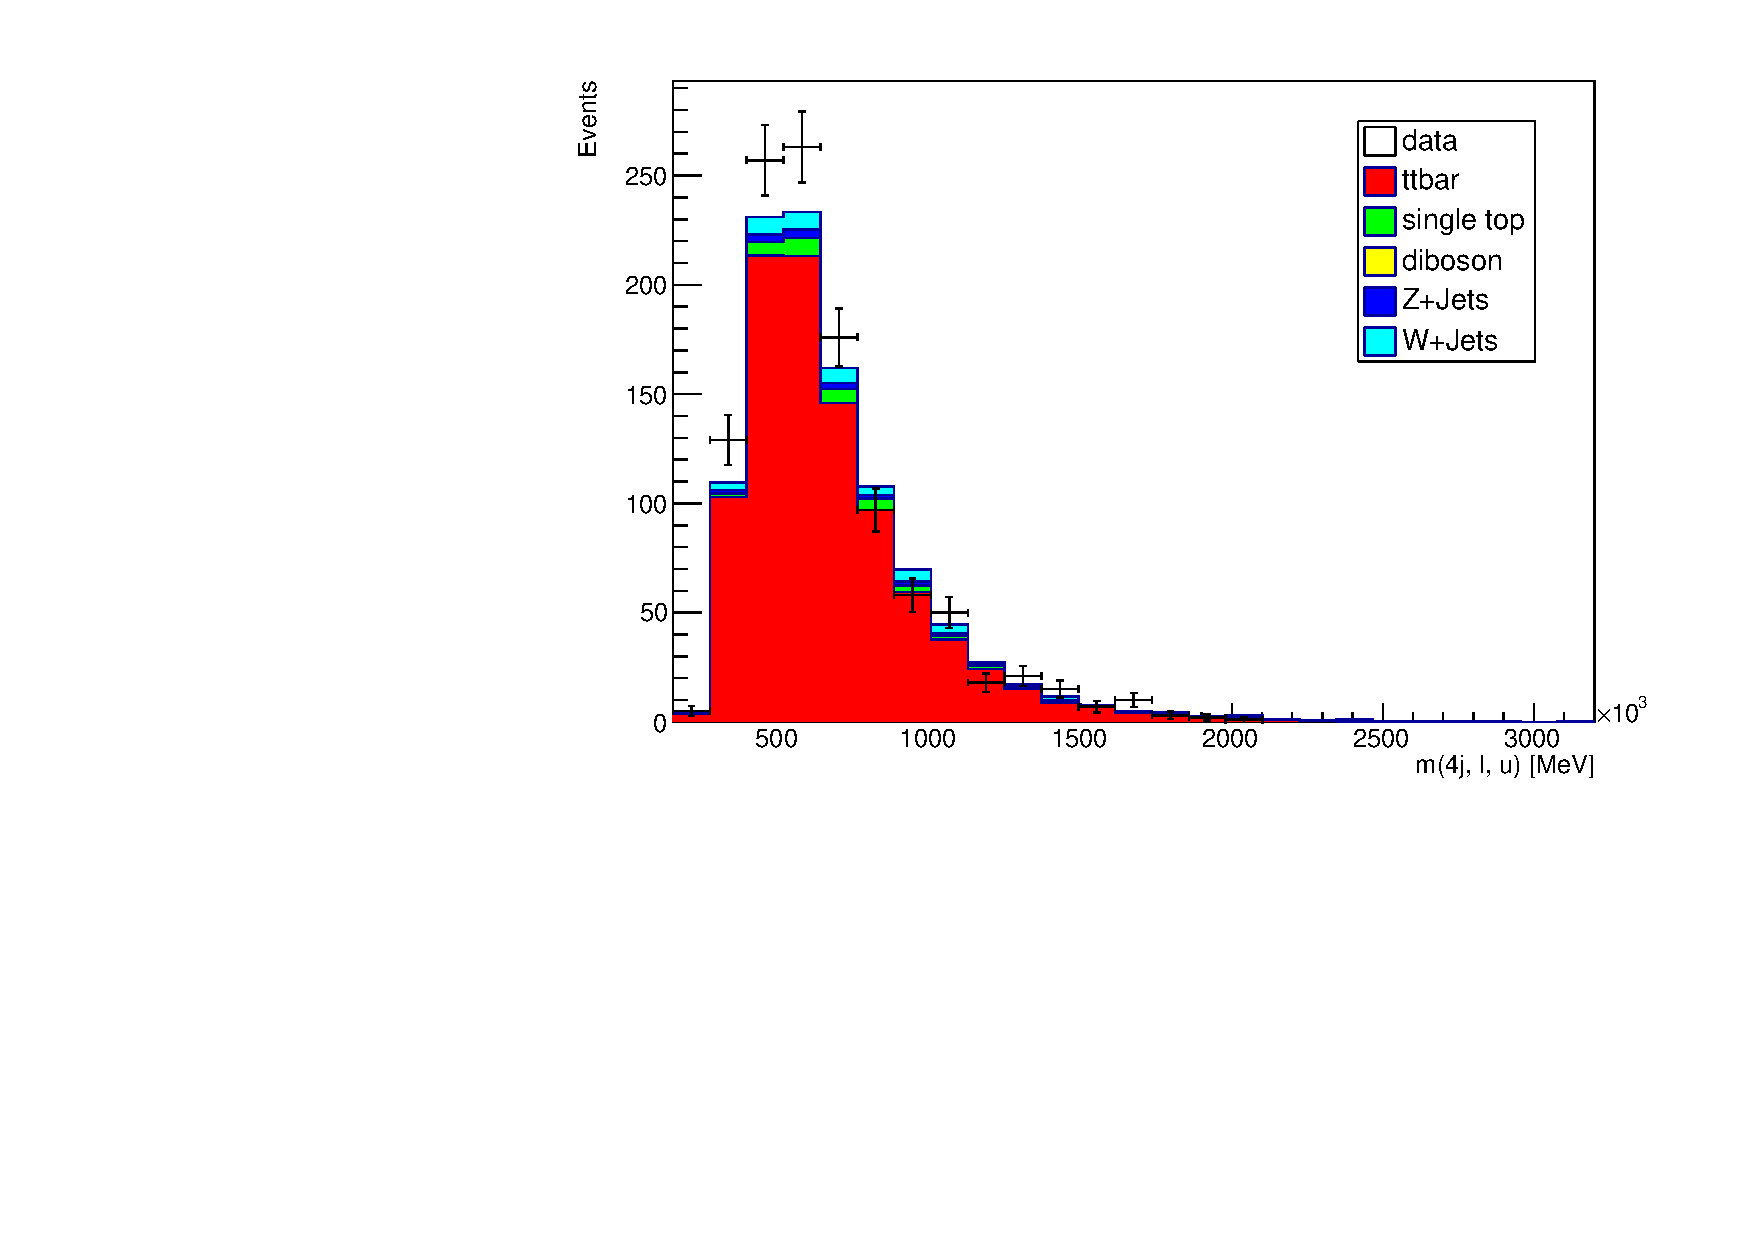
\includegraphics[width=.6\textwidth]{plots/comparism/m_event.pdf}
  \caption{Stacked plot of the chosen discriminant.}
  \label{fig:7}
\end{figure}


\subsection{Statistical analysis}
To investigate the agreement of the simulated samples and the data samples quantitatively the $\chi^2$ value for between the distribution of the 
data sample and the sum of the simulated background samples is determined for the chosen final discriminant. Furthermore the p-value $p$ and the 
confidence level $\text{CL} = 1-p$ is determined. If $p$ would be found to be smaller than $0.05$ the deviation observed between data and simulation of the 
backgrounds from the standard model would be seen as statistically significant. The values are found to be 
\begin{align*}
  \chi^2 &= 32.9652 \\
  p &= 0.131945
\end{align*}
and therefore the deviation is not statistically significant. 
To further investigate the possibility of a $Z^\prime$ signal in the data a $95 \%$ exclusion limit for the different mass hypothesis 
is determined by varying the crosssection with a parameter $s$ and replacing the cross section in the weights to be $\sigma^\prime = s \sigma$ 
until the p-value between the sum of the simulated standard model processes and $Z^\prime$ and the data samples in the final disciminant is 
$\approx 0.05$. The values found this way for the parameter $s$ and the new cross section for the different mass hypothesis are listed in table \ref{tab:lim}. 
Furthermore the cross sections $\sigma^\prime$ at the $95 \%$ confidence level and the predicted cross sections are plotted against the mass of $Z^\prime$ 
in figure \ref{fig:sigm}.
% chi square background only 32.9652

\begin{table}[H]
  \centering
  \begin{tabular}{l|llll}
      sample           &  $\chi^2_{25}$  & $s$ & $\sigma^\prime \, / \, \si{\pico\barn}$ \\
      \hline
      zprime400  &   37.7281   &          1.15                      & 126.5           \\
      zprime500  &   37.0327   &          0.57                      & 46.74           \\
      zprime750  &   37.5158   &          0.430001                      & 8.60001         \\
      zprime1000 &   37.0651   &          0.0700007                      & 0.385004        \\
      zprime1250 &   37.6404   &          0.220001                      & 0.418001        \\
      zprime1500 &   37.4218   &          0.410001                      & 0.3403          \\
      zprime1750 &   37.626    &          0.9                      & 0.27            \\
      zprime2000 &   37.6757   &          1.82                      & 0.2548          \\
      zprime2250 &   37.6524   &          35.97                      & 2.40999         \\
      zprime2500 &   37.4851   &          61.6557                      & 2.15795         \\
      zprime3000 &   32.981    &          1.01                      & 0.01212         \\
      \end{tabular}
\caption{The efficiency of the selection after the application of subsequent cuts (6-7).}
\label{tab:lim}

  \end{table}




  \begin{figure}[tb]
    \centering
    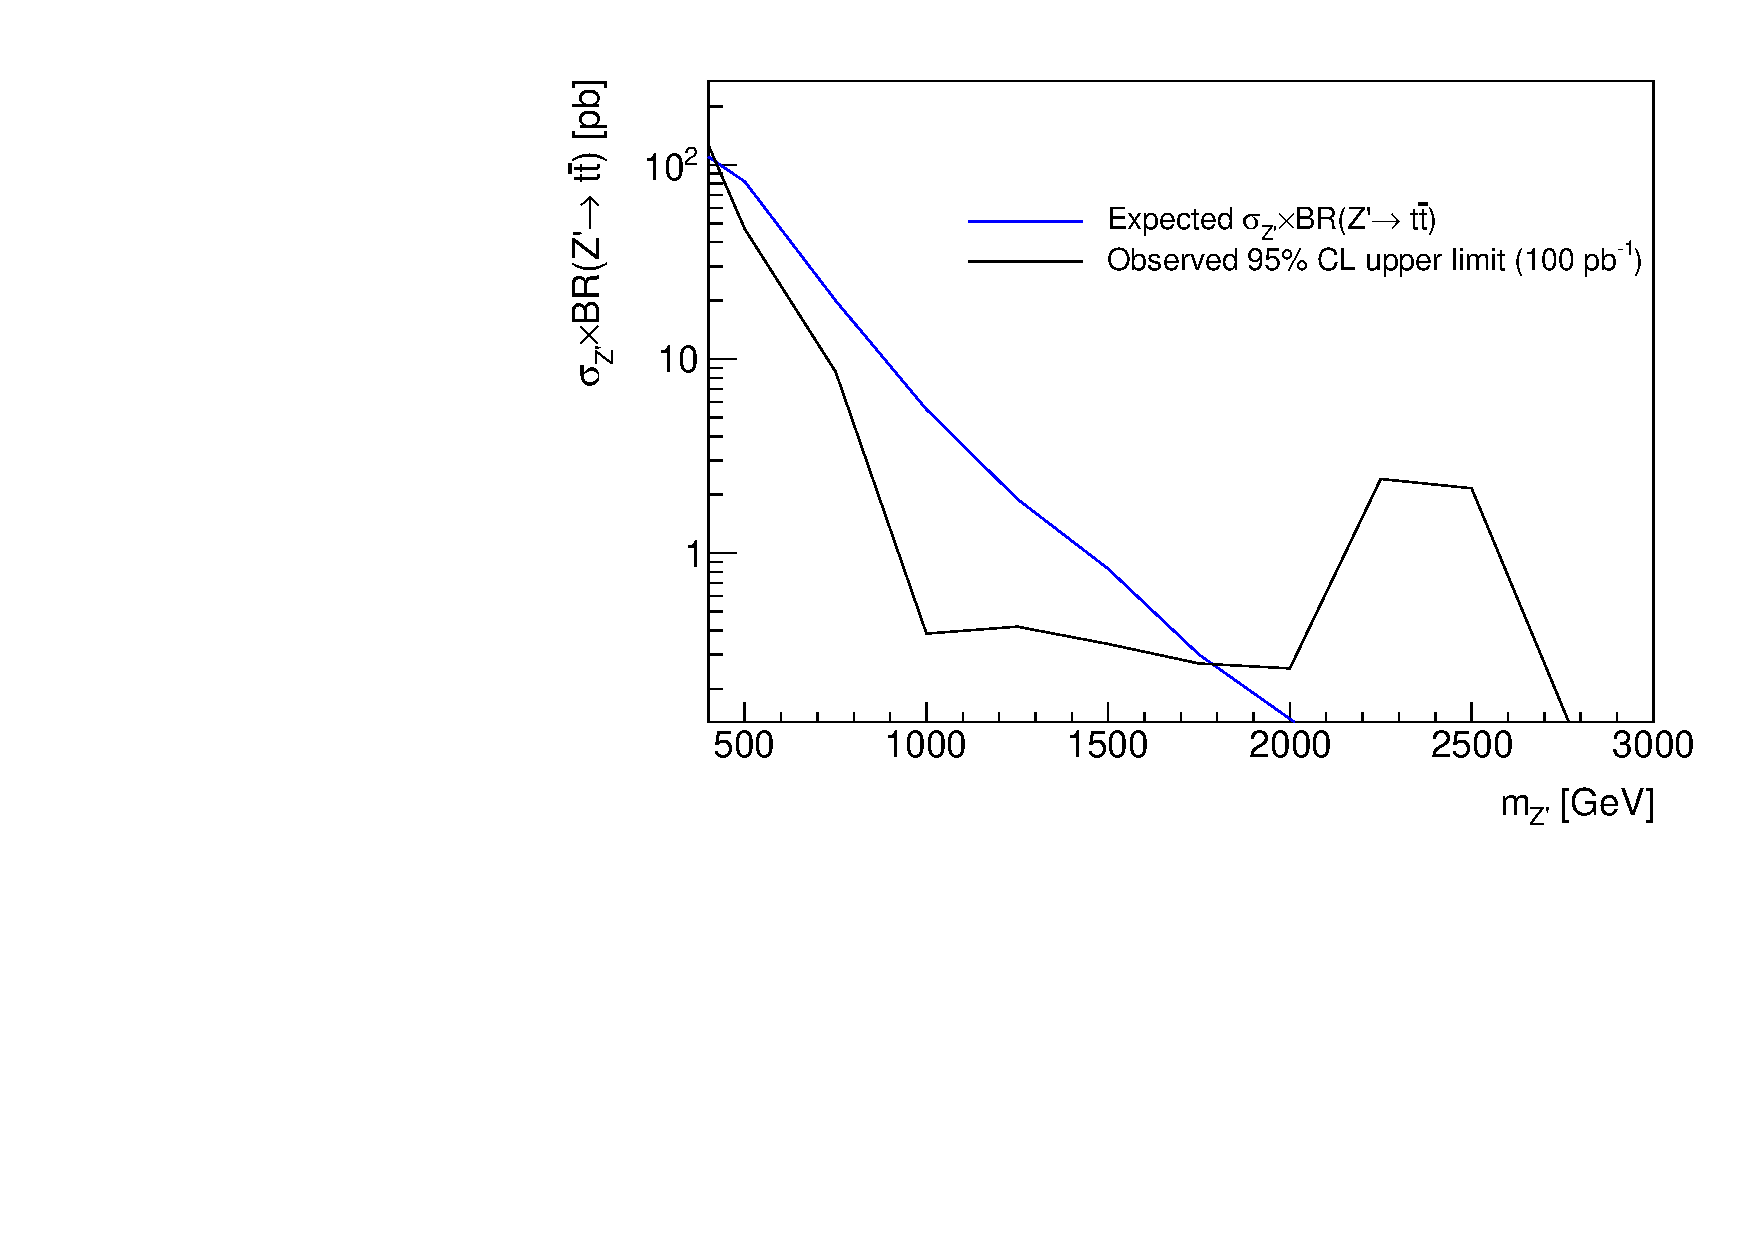
\includegraphics[width=.9\textwidth]{plots/limits.pdf}
    \caption{Histogram of the transverse momentum of the leptons in from one of the data samples created with the \texttt{TBrowser} environment from \texttt{Root}.}
    \label{fig:sigm}
  \end{figure}